% Options for packages loaded elsewhere
\PassOptionsToPackage{unicode}{hyperref}
\PassOptionsToPackage{hyphens}{url}
%
\documentclass[
]{book}
\usepackage{lmodern}
\usepackage{amssymb,amsmath}
\usepackage{ifxetex,ifluatex}
\ifnum 0\ifxetex 1\fi\ifluatex 1\fi=0 % if pdftex
  \usepackage[T1]{fontenc}
  \usepackage[utf8]{inputenc}
  \usepackage{textcomp} % provide euro and other symbols
\else % if luatex or xetex
  \usepackage{unicode-math}
  \defaultfontfeatures{Scale=MatchLowercase}
  \defaultfontfeatures[\rmfamily]{Ligatures=TeX,Scale=1}
\fi
% Use upquote if available, for straight quotes in verbatim environments
\IfFileExists{upquote.sty}{\usepackage{upquote}}{}
\IfFileExists{microtype.sty}{% use microtype if available
  \usepackage[]{microtype}
  \UseMicrotypeSet[protrusion]{basicmath} % disable protrusion for tt fonts
}{}
\makeatletter
\@ifundefined{KOMAClassName}{% if non-KOMA class
  \IfFileExists{parskip.sty}{%
    \usepackage{parskip}
  }{% else
    \setlength{\parindent}{0pt}
    \setlength{\parskip}{6pt plus 2pt minus 1pt}}
}{% if KOMA class
  \KOMAoptions{parskip=half}}
\makeatother
\usepackage{xcolor}
\IfFileExists{xurl.sty}{\usepackage{xurl}}{} % add URL line breaks if available
\IfFileExists{bookmark.sty}{\usepackage{bookmark}}{\usepackage{hyperref}}
\hypersetup{
  pdftitle={Getting started with Quantitative Research Methods and R},
  pdfauthor={Lukas Wallrich},
  hidelinks,
  pdfcreator={LaTeX via pandoc}}
\urlstyle{same} % disable monospaced font for URLs
\usepackage{color}
\usepackage{fancyvrb}
\newcommand{\VerbBar}{|}
\newcommand{\VERB}{\Verb[commandchars=\\\{\}]}
\DefineVerbatimEnvironment{Highlighting}{Verbatim}{commandchars=\\\{\}}
% Add ',fontsize=\small' for more characters per line
\usepackage{framed}
\definecolor{shadecolor}{RGB}{248,248,248}
\newenvironment{Shaded}{\begin{snugshade}}{\end{snugshade}}
\newcommand{\AlertTok}[1]{\textcolor[rgb]{0.94,0.16,0.16}{#1}}
\newcommand{\AnnotationTok}[1]{\textcolor[rgb]{0.56,0.35,0.01}{\textbf{\textit{#1}}}}
\newcommand{\AttributeTok}[1]{\textcolor[rgb]{0.77,0.63,0.00}{#1}}
\newcommand{\BaseNTok}[1]{\textcolor[rgb]{0.00,0.00,0.81}{#1}}
\newcommand{\BuiltInTok}[1]{#1}
\newcommand{\CharTok}[1]{\textcolor[rgb]{0.31,0.60,0.02}{#1}}
\newcommand{\CommentTok}[1]{\textcolor[rgb]{0.56,0.35,0.01}{\textit{#1}}}
\newcommand{\CommentVarTok}[1]{\textcolor[rgb]{0.56,0.35,0.01}{\textbf{\textit{#1}}}}
\newcommand{\ConstantTok}[1]{\textcolor[rgb]{0.00,0.00,0.00}{#1}}
\newcommand{\ControlFlowTok}[1]{\textcolor[rgb]{0.13,0.29,0.53}{\textbf{#1}}}
\newcommand{\DataTypeTok}[1]{\textcolor[rgb]{0.13,0.29,0.53}{#1}}
\newcommand{\DecValTok}[1]{\textcolor[rgb]{0.00,0.00,0.81}{#1}}
\newcommand{\DocumentationTok}[1]{\textcolor[rgb]{0.56,0.35,0.01}{\textbf{\textit{#1}}}}
\newcommand{\ErrorTok}[1]{\textcolor[rgb]{0.64,0.00,0.00}{\textbf{#1}}}
\newcommand{\ExtensionTok}[1]{#1}
\newcommand{\FloatTok}[1]{\textcolor[rgb]{0.00,0.00,0.81}{#1}}
\newcommand{\FunctionTok}[1]{\textcolor[rgb]{0.00,0.00,0.00}{#1}}
\newcommand{\ImportTok}[1]{#1}
\newcommand{\InformationTok}[1]{\textcolor[rgb]{0.56,0.35,0.01}{\textbf{\textit{#1}}}}
\newcommand{\KeywordTok}[1]{\textcolor[rgb]{0.13,0.29,0.53}{\textbf{#1}}}
\newcommand{\NormalTok}[1]{#1}
\newcommand{\OperatorTok}[1]{\textcolor[rgb]{0.81,0.36,0.00}{\textbf{#1}}}
\newcommand{\OtherTok}[1]{\textcolor[rgb]{0.56,0.35,0.01}{#1}}
\newcommand{\PreprocessorTok}[1]{\textcolor[rgb]{0.56,0.35,0.01}{\textit{#1}}}
\newcommand{\RegionMarkerTok}[1]{#1}
\newcommand{\SpecialCharTok}[1]{\textcolor[rgb]{0.00,0.00,0.00}{#1}}
\newcommand{\SpecialStringTok}[1]{\textcolor[rgb]{0.31,0.60,0.02}{#1}}
\newcommand{\StringTok}[1]{\textcolor[rgb]{0.31,0.60,0.02}{#1}}
\newcommand{\VariableTok}[1]{\textcolor[rgb]{0.00,0.00,0.00}{#1}}
\newcommand{\VerbatimStringTok}[1]{\textcolor[rgb]{0.31,0.60,0.02}{#1}}
\newcommand{\WarningTok}[1]{\textcolor[rgb]{0.56,0.35,0.01}{\textbf{\textit{#1}}}}
\usepackage{longtable,booktabs}
% Correct order of tables after \paragraph or \subparagraph
\usepackage{etoolbox}
\makeatletter
\patchcmd\longtable{\par}{\if@noskipsec\mbox{}\fi\par}{}{}
\makeatother
% Allow footnotes in longtable head/foot
\IfFileExists{footnotehyper.sty}{\usepackage{footnotehyper}}{\usepackage{footnote}}
\makesavenoteenv{longtable}
\usepackage{graphicx,grffile}
\makeatletter
\def\maxwidth{\ifdim\Gin@nat@width>\linewidth\linewidth\else\Gin@nat@width\fi}
\def\maxheight{\ifdim\Gin@nat@height>\textheight\textheight\else\Gin@nat@height\fi}
\makeatother
% Scale images if necessary, so that they will not overflow the page
% margins by default, and it is still possible to overwrite the defaults
% using explicit options in \includegraphics[width, height, ...]{}
\setkeys{Gin}{width=\maxwidth,height=\maxheight,keepaspectratio}
% Set default figure placement to htbp
\makeatletter
\def\fps@figure{htbp}
\makeatother
\setlength{\emergencystretch}{3em} % prevent overfull lines
\providecommand{\tightlist}{%
  \setlength{\itemsep}{0pt}\setlength{\parskip}{0pt}}
\setcounter{secnumdepth}{5}
\usepackage{booktabs}

\newenvironment{danger}
    {
    \hline\\
    }
    { 
    \\\\\hline
    }
    
\newenvironment{warning}
    {
    \hline\\
    }
    { 
    \\\\\hline
    }
    
\newenvironment{info}
    {
    \hline\\
    }
    { 
    \\\\\hline
    }
    
\newenvironment{try}
    {
    \hline\\
    }
    { 
    \\\\\hline
    }
\usepackage{amsmath}
\usepackage{booktabs}
\usepackage{caption}
\usepackage{longtable}
\usepackage[]{natbib}
\bibliographystyle{apalike}

\title{Getting started with Quantitative Research Methods and R}
\author{Lukas Wallrich}
\date{Last updated: 2021-02-01}

\begin{document}
\maketitle

{
\setcounter{tocdepth}{1}
\tableofcontents
}
\hypertarget{overview}{%
\chapter*{Overview}\label{overview}}
\addcontentsline{toc}{chapter}{Overview}

This guide supports the Core Quantitative Methods Course offered by the Goldsmiths' Graduate School. \textbf{It is a living document and currently focuses on R at the expense of broader considerations of quantitative research, but will grow over time - \href{https://github.com/LukasWallrich/GoldCoreQuants/issues}{please raise any issues and suggestions here}.} It does not follow the order of sessions in the course; instead, it is ordered in a way that might allow you to see connections and hopefully helps to look things up more easily.

\hypertarget{further-sources}{%
\section{Further sources}\label{further-sources}}

This guide does not aim to be comprehensive, but just to provide sufficient orientation. There are many fantastic free online resources that go further.

\hypertarget{free-online-books}{%
\subsection{Free online books}\label{free-online-books}}

\begin{itemize}
\tightlist
\item
  Hadley Wickham, the leading brain behind the \texttt{tidyverse} packages, has co-authored \href{https://r4ds.had.co.nz/index.html}{\emph{R for Data Science}} (with Garrett Grolemund). This book does not cover inferential statistics, but explains how to use R to process, describe and visualise data in line with the aproach taken in this course.
\item
  The \href{https://learningstatisticswithr.com/book/}{\emph{Learning statistics with R}} book by Danielle Navarro focuses on explaining the different statistical tests and their application in quite a lot of detail, including the underlying maths. It is written by a psychologist, and might therefore be particularly helpful for people from that discipline.
\item
  \href{https://statsthinking21.github.io/statsthinking21-core-site/}{Statistical thinking for the 21st century} is a great modern book on statistics, which also offers this handy \href{https://statsthinking21.github.io/statsthinking21-R-site/index.html}{R companion} that covers most of what is needed for this course (though it is still a work-in-progress document).
\end{itemize}

\hypertarget{paperlibrary-books}{%
\subsection{Paper/library books}\label{paperlibrary-books}}

\begin{itemize}
\tightlist
\item
  Charles Wheelan's \emph{Naked Statistics: Stripping the Dread from the Data} is an easy-to-read and entertaining New York Times bestseller that introduces statistical thinking and some key concepts without distracting details.
\item
  Neil Burdess' \emph{Starting Statistics: A short clear guide} covers the basic ground with more practical and technical detail.
\item
  Also have a look at the \textbf{Module Guide} on the \href{https://learn.gold.ac.uk/}{learn.gold} Module Page that contains further recommendations, especially with regard to research methods.
\end{itemize}

\hypertarget{other-key-resources}{%
\subsection{Other key resources}\label{other-key-resources}}

\begin{itemize}
\tightlist
\item
  The RStudio team created and collected a very helpful set of Cheat Sheets that cover the key elements of various R packages - have a look \href{https://rstudio.com/resources/cheatsheets/}{here.} For this course, the sheets on \texttt{dplyr} and \texttt{ggplot2} are the most important.
\item
  \href{https://stackoverflow.com/questions/tagged/r}{Stackoverflow} is an online forum with a knewledgeable and welcoming support community. However, make sure to use Google and their search function first to check that your question hasn't already been answered and show what you already understand - if the same questions keep on getting asked or if the questions are very unclear, people volunteering their time to help can get a bit testy.
\end{itemize}

\hypertarget{why-r}{%
\section{Why R?}\label{why-r}}

R is not the easiest statistical software to learn, but we are confident that it is the most useful. This \href{https://lindeloev.net/spss-is-dying/}{article} on why SPSS is dying provides some arguments for why that is the case, while Andy Fields (a leading stats teacher and textbook author) offers his case for learning R \href{https://padlet-uploads.storage.googleapis.com/290004173/0ce387ac71c38e2643953a2148c0cd81/why_r.html}{here}.

\hypertarget{part-using-r-and-describing-data}{%
\part*{Using R and describing data}\label{part-using-r-and-describing-data}}
\addcontentsline{toc}{part}{Using R and describing data}

\hypertarget{getting-started-with-r}{%
\chapter{Getting started with R}\label{getting-started-with-r}}

\hypertarget{install-r-on-your-computer}{%
\section{Install R on your computer}\label{install-r-on-your-computer}}

R is highly customizable, so that your life is a lot easier if you use your own copy rather than a shared copy on a university computer. To install it on your computer, follow the detailed instructions in \href{https://r4ds.had.co.nz/introduction.html}{Section 1.4 of the R for Data Science book}

Then \textbf{start exploring} - using R is a skill that comes with practice, not with reading about it. The examples from these notes can be copy-pasted or typed into R (when you move the mouse pointer over a code box you should see a copy-button in the top-right corner).

\hypertarget{some-key-concepts}{%
\section{Some key concepts}\label{some-key-concepts}}

If you understand the following concepts, using R will make a lot more sense.

\hypertarget{r-rstudio-and-r-packages}{%
\subsection{R, RStudio and R packages}\label{r-rstudio-and-r-packages}}

You can think about the different parts of R in terms of a computer or smartphone. In that analogy:

\begin{itemize}
\item
  \textbf{R is the processor and operating system} that carries out everything under the hood. It also contains many basic functions (i.e.~commands) for everyday tasks
\item
  \textbf{RStudio is the user interface.} The following parts are most relevant:

  \begin{itemize}
  \tightlist
  \item
    \textbf{Console} to type and run commands (usually to try things out or do things that need to be done once only)
  \item
    \textbf{File editor} to develop production code (i.e.~code needed to reproduce your analyses and create reports). Here you edit .Rmd files (or plain .R scripts, which are not used in this course)
  \item
    \textbf{Environment} shows a list of all variables you have created. For dataframes, it shows the number of observations (rows) and variables (columns). Clicking on the name opens the data, clicking on the arrow shows some details
  \item
    \textbf{History} is a searchable list of all commands you have run - helpful if you want to reuse something you have done a while back.
  \end{itemize}
\item
  \textbf{R packages are the apps}

  \begin{itemize}
  \tightlist
  \item
    Installed once, using \texttt{install.packages("name")}
  \item
    Loaded in every session, using \texttt{library(name)}
  \end{itemize}
\end{itemize}

For a more comprehensive introduction to R, you can watch this video:

\hypertarget{data-and-variables-in-r}{%
\subsection{Data and variables in R}\label{data-and-variables-in-r}}

Lines starting with a \# are comments that are ignored by R. I use them below to explain parts of the code further.

\begin{Shaded}
\begin{Highlighting}[]
\CommentTok{# <- saves a value (on the right) into an object (on the left)}
\NormalTok{score <-}\StringTok{ }\DecValTok{10}

\CommentTok{# "" need to be used around text that is not an object name}
\NormalTok{month <-}\StringTok{ "January"} 

\CommentTok{# c() combines several values into one vector that }
\CommentTok{# can then be saved as a single object}
\NormalTok{weekend <-}\StringTok{ }\KeywordTok{c}\NormalTok{(}\StringTok{"Saturday"}\NormalTok{, }\StringTok{"Sunday"}\NormalTok{) }
\NormalTok{sleep_hours <-}\StringTok{ }\KeywordTok{c}\NormalTok{(}\DecValTok{4}\NormalTok{, }\DecValTok{9}\NormalTok{)}

\CommentTok{#Variables can then be combined into dataframes (R's version of tables)}
\NormalTok{sleep_data <-}\StringTok{ }\KeywordTok{data.frame}\NormalTok{(}\DataTypeTok{day =}\NormalTok{ weekend, }\DataTypeTok{hours =}\NormalTok{ sleep_hours)}

\CommentTok{#Variables within dataframes are accessed using the $ operator}
\KeywordTok{sum}\NormalTok{(sleep_data}\OperatorTok{$}\NormalTok{hours)}
\end{Highlighting}
\end{Shaded}

\begin{verbatim}
## [1] 13
\end{verbatim}

\textbf{Variable classes} indicate what kind of data a variable contains. There are four main types

\begin{itemize}
\tightlist
\item
  numeric, integer or double (i.e.~numbers, the differences are not relevant to us)
\item
  character, i.e.~any text
\item
  logical, i.e.~TRUE/FALSE values
\item
  and factors, i.e.~categorical variables, for example weekdays.
\end{itemize}

The \texttt{class()} function shows the class of a single variable, the \texttt{str()} and \texttt{glimpse()} functions include the classes of all variables in a dataframe.

Usually, R gets the classes right by itself and converts as required. If you need to change variable classes, you can use the \texttt{as.numeric()}, \texttt{as.character()}, \texttt{as.logical()}, \texttt{as.factor()} etc. functions.

\begin{Shaded}
\begin{Highlighting}[]
\KeywordTok{class}\NormalTok{(sleep_data}\OperatorTok{$}\NormalTok{hours)}
\KeywordTok{str}\NormalTok{(sleep_data)}
\end{Highlighting}
\end{Shaded}

\begin{verbatim}
## [1] "numeric"
## 'data.frame':	2 obs. of  2 variables:
##  $ day  : chr  "Saturday" "Sunday"
##  $ hours: num  4 9
\end{verbatim}

\hypertarget{functions-in-r}{%
\subsection{Functions in R}\label{functions-in-r}}

All work in R is based on calling functions that do something. A function is called by its name with () behind. If you just type the name, the function is printed out - you usually don't want this.

\begin{Shaded}
\begin{Highlighting}[]
\CommentTok{#Some functions work without any additional arguments}
\KeywordTok{timestamp}\NormalTok{() }\CommentTok{#This shows the time this code segment was run}

\CommentTok{#Functions that work with given data are more helpful - }
\CommentTok{# that data is given as an 'argument' in brackets}
\KeywordTok{print}\NormalTok{(}\StringTok{"Hello"}\NormalTok{)}
\KeywordTok{mean}\NormalTok{(}\KeywordTok{c}\NormalTok{(}\DecValTok{1}\NormalTok{,}\DecValTok{2}\NormalTok{,}\DecValTok{3}\NormalTok{))}

\CommentTok{#Additionally, arguments can contain instructions to the function}
\KeywordTok{mean}\NormalTok{(}\KeywordTok{c}\NormalTok{(}\DecValTok{1}\NormalTok{,}\DecValTok{2}\NormalTok{,}\DecValTok{3}\NormalTok{, }\OtherTok{NA}\NormalTok{), }\DataTypeTok{na.rm =} \OtherTok{TRUE}\NormalTok{)}
\CommentTok{# NA is a missing value, na.rm tells the mean function to remove it }
\CommentTok{# before calculating the mean}

\CommentTok{#To save the results of a function into a variable, use the <- operator again}
\NormalTok{variableName <-}\StringTok{ }\KeywordTok{mean}\NormalTok{(}\KeywordTok{c}\NormalTok{(}\DecValTok{1}\NormalTok{,}\DecValTok{2}\NormalTok{,}\DecValTok{3}\NormalTok{, }\OtherTok{NA}\NormalTok{), }\DataTypeTok{na.rm =} \OtherTok{TRUE}\NormalTok{)}
\end{Highlighting}
\end{Shaded}

\begin{verbatim}
## ##------ Mon Feb  1 12:42:41 2021 ------##
## [1] "Hello"
## [1] 2
## [1] 2
\end{verbatim}

To learn more about the arguments accepted by a specific function, use the \texttt{?} command to open the help page, e.g., by typing \texttt{?mean}. Arguments are matched by their name, as with \texttt{na.rm\ =} above; if no name is given, they are matched by their position in the function call. Usually, only very common arguments, typically the data, should be left unnamed.

\hypertarget{key-r-packages}{%
\subsection{Key R packages}\label{key-r-packages}}

The most essential packages for this course are included in the \texttt{tidyverse} - a whole set of packages to make data manipulation and visualisation in R efficient and consistent. They include:

\begin{itemize}
\tightlist
\item
  \texttt{dplyr}: a package to efficiently manipulate data and create summary statistics
\item
  \texttt{ggplot2}: a package to create all kinds of graphs
\item
  \texttt{readr}: a package to load table data into R that is formatted as text
\end{itemize}

All these packages are loaded with the \texttt{library(tidyverse)} command. There are some additional packages in the tidyverse that need to be loaded separately, using \texttt{library(packagename)}. The most relevant for us are:

\begin{itemize}
\tightlist
\item
  \texttt{readxl} and \texttt{haven}: package to load data from Excel and statistical software
\item
  \texttt{stringr}: a package to manipulate strings
\item
  \texttt{lubridate}: a package to convert, filter and analyse times and dates
\end{itemize}

\hypertarget{using-the-pacman-package}{%
\subsubsection{\texorpdfstring{Using the \texttt{pacman} package}{Using the pacman package}}\label{using-the-pacman-package}}

As an alternative to \texttt{install.packages()} and \texttt{library()}, you can also use the \texttt{p\_load} function in the \texttt{pacman} package. That function checks first whether the package is installed, installs it if needed, and then loads it. I am using it in the code here so that you easily copy-paste parts of it; in your own code, the choice is up to you. If you want to use \texttt{pacman}, just run \texttt{install.packages("pacman")} and then use \texttt{pacman::p\_load(package1,\ package2)} to load your packages.

\hypertarget{using-a-single-function-in-a-package}{%
\subsubsection{Using a single function in a package}\label{using-a-single-function-in-a-package}}

If you just need to use one function from a package, you do not need to load the whole package. You can also give R the whole address and use \texttt{package::function()}. I will only do that for \texttt{pacman::p\_load()} since that is the only function from that package we will ever use in this course.

\hypertarget{rmarkdown}{%
\subsection{RMarkdown}\label{rmarkdown}}

A key strength of R are \textbf{reproducible analyses.} For that, we don't want to type commands and just write down the results, but rather create scripts that can produce results again and again. That also makes changes much less painful, for instance if you've made a mistake at the start.

\textbf{RMarkdown (.Rmd)} files are such scripts that additionally allow to add text and split the code into separate chunks. Within them, \emph{grey chunks} are code, anything else is not executed. It is just formatted (e.g., with headings and highlights) when you create the report. Markup symbols allow for easy formatting of the text, as per the instructions \href{https://rmarkdown.rstudio.com/authoring_basics.html}{here}. (Most of that is not required in this course, a couple of key symbols such as \# to indicate headings will be introduced later.)

Within \emph{.Rmd} files, you need to \textbf{Insert} new code blocks for the major parts of the analysis. For that, use the insert button at the top of the File Editor window. When you want to test your code, you can also \textbf{Run} it there or by pressing \emph{Ctrl+Enter} in the line you want to use (or after you have selected multiple lines to run). Finally, to create the report you need to \textbf{Knit} it, again using the button in the File Editor Without installing anything else, you can only knit to \emph{HTML files}, but those can be opened in any internet browser, so are good to share with anyone.

\hypertarget{help-what-to-do-when-problems-appear}{%
\subsection{HELP! What to do when problems appear?}\label{help-what-to-do-when-problems-appear}}

When \textbf{red text} appears in the console, don't panick. Some messages that are often entirely irrelevant are displayed in red, for example when packages are loaded. \textbf{Warnings} are more important, but they just alert you that something might be going wrong - read them, but then decide whether you need to worry. For instance, ggplot prints a warning when data is missing, which might or might not be a problem for you. Only \textbf{Errors} always need to be dealt with as they stop your commands from being executed and the .Rmd file from being knitted. Unfortunately, many R functions give rather cryptic error messages - if you are stuck, first check your code for typos, then Google the error message.

Many errors occur due to \textbf{common mistakes}, that you need to pay attention to:

\begin{itemize}
\tightlist
\item
  \textbf{Missing brackets} - make sure each \texttt{(} is matched by a \texttt{)} in the right place. When your cursor is at a closing bracket, R highlights the opening bracket it is matched with, which helps to check your syntax
\item
  \textbf{Misspellings} - variable names and functions need to be spelled correctly, which includes capitalisation, otherwise you might inadvertently create duplicates or cause other issues. Some functions are available in both American and British spelling (e.g., \texttt{summarise()}and \texttt{summarize()} in dplyr), but this is not always the case so that it might be sensible to always stick to American spelling
\item
  \textbf{Missing library() calls} to load packages - if a function is not found, run \texttt{library(packagename)}
\item
  \textbf{Function masking} - many packages have functions of the same name, so that packages that are loaded later mask (i.e.~``over-write'') the names of functions in packages loaded earlier (for example, dplyr's \texttt{filter()} function masks the \texttt{filter()} function in base R). Often, that is exactly what we want, but if a function does not do what you expect it to do, it's worth specifying the package it comes from to make sure you are not actually calling a different function that has masked it. You can do that by adding the package name and \texttt{::}, for example, by calling \texttt{dplyr::filter()} \emph{Note}: If you only want to use a single function from a large package, this is an alternative to loading the full package.
\end{itemize}

As you progress in R, \textbf{do not try to remember everything} - instead, look things up as needed, in particular things like argument names:

\begin{itemize}
\tightlist
\item
  Use \texttt{?functionName} to get help in R
\item
  Refer to the \href{https://rstudio.com/resources/cheatsheets/}{RStudio Cheatsheets}
\item
  Google your questions and pay particular attention to results from r-bloggers.com and stackoverflow.com
\end{itemize}

There is also a very active R user community that is willing to help - \href{https://stackoverflow.com/}{stackoverflow.com} is a good place to ask questions about R Code, while \href{https://stats.stackexchange.com}{stats.stackexchange.com} is the place to go with questions that are more generally about statistics. In both cases, it pays off to first google and then post questions that are as specific as possible.

\hypertarget{importing-and-describing-data}{%
\chapter{Importing and describing data}\label{importing-and-describing-data}}

\hypertarget{importing-data-into-r}{%
\section{Importing data into R}\label{importing-data-into-r}}

Generally, R is a poor choice for data entry, so you will usually import data from spreadsheet software or other sources. That also helps to keep data and analyses apart, and thereby increases transparency.

The most common ways to import data into R are to

\begin{itemize}
\tightlist
\item
  read tabular data saved as text (such as the common \emph{.csv} files) with the \texttt{readr} package
\item
  read Excel files with the \texttt{readxl} package
\item
  read data files from SPSS or SAS with \texttt{haven}.
\end{itemize}

In these packages, the functions to read data are always \texttt{read\_x()}, with x replaced by the type of file you want to open. You always need to specify the name of the datafile, with its path (unless it is in the same folder as your .Rmd file), as the first argument of the \texttt{read\_x()} function. For the path, it can be helpful to start with the dot (\texttt{.}), which means: start from the current folder. For example, I often have a data folder within the folder where the .Rmd file is, so that the path would then be \texttt{"./data/file.csv"}. Always remember to assign the result of the function (i.e.~the data) to a variable using \texttt{\textless{}-}, otherwise the data is just printed and not saved in R.

The functions that load data from tables need to establish the variable class for each variable. They can either guess (which you will then need to check), or you can provide the classes in the \texttt{col\_types}-argument. Check \texttt{?readr::read\_csv} for details.

\begin{Shaded}
\begin{Highlighting}[]
\CommentTok{#readr is loaded with the tidyverse, but can be loaded separately }
\CommentTok{#as well if you don't need the other packages}
\NormalTok{pacman}\OperatorTok{::}\KeywordTok{p_load}\NormalTok{(readr)}
\NormalTok{gapminder <-}\StringTok{ }\KeywordTok{read_csv}\NormalTok{(}\StringTok{"./data/gapminder.csv"}\NormalTok{, }\DataTypeTok{col_types =} \StringTok{"finnnnnff"}\NormalTok{)}

\NormalTok{pacman}\OperatorTok{::}\KeywordTok{p_load}\NormalTok{(readxl)}
\NormalTok{gapminder <-}\StringTok{ }\KeywordTok{read_xlsx}\NormalTok{(}\StringTok{"./data/gapminder.xlsx"}\NormalTok{) }
\CommentTok{# Here col_types are not defined so that R will guess and print }
\CommentTok{# out the results - make sure to check whether the classes are }
\CommentTok{# what you would expect}

\NormalTok{pacman}\OperatorTok{::}\KeywordTok{p_load}\NormalTok{(haven)}
\NormalTok{gapminder <-}\StringTok{ }\KeywordTok{read_sav}\NormalTok{(}\StringTok{"./data/gapminder.sav"}\NormalTok{) }
\CommentTok{#SPSS files contain information on the class of each variable, }
\CommentTok{#so that col_types do not need to be defined}
\end{Highlighting}
\end{Shaded}

There are shortcuts to quickly get some data into R, which can be helpful if you just want to try something out - all of them only make sense in the Console, not in a .Rmd script. Using the \texttt{edit()} function, you can open up a simple spreadsheet to edit and input data, using \texttt{read.table(file="clipboard",\ sep="\textbackslash{}t")}, you can get data you copied in Excel. As with all ways of importing data, remember to assign the result to a variable.

\begin{Shaded}
\begin{Highlighting}[]
\CommentTok{#If you want to edit an existing dataset}
\NormalTok{gapminder_corrected <-}\StringTok{ }\KeywordTok{edit}\NormalTok{(gapminder)}

\CommentTok{#If you want to type or copy in a new dataset}
\NormalTok{yourdata <-}\StringTok{ }\KeywordTok{edit}\NormalTok{(}\KeywordTok{data.frame}\NormalTok{())}
\CommentTok{#The data.frame() function creates an empty dataframe for you to then edit}

\CommentTok{#If you want to read data from the clipboard}
\NormalTok{pasted <-}\StringTok{ }\KeywordTok{read.table}\NormalTok{(}\DataTypeTok{file=}\StringTok{"clipboard"}\NormalTok{, }\DataTypeTok{sep=}\StringTok{"}\CharTok{\textbackslash{}t}\StringTok{"}\NormalTok{)}

\CommentTok{#If that data contains variable names in the first row:}
\NormalTok{pasted <-}\StringTok{ }\KeywordTok{read.table}\NormalTok{(}\DataTypeTok{file=}\StringTok{"clipboard"}\NormalTok{, }\DataTypeTok{sep=}\StringTok{"}\CharTok{\textbackslash{}t}\StringTok{"}\NormalTok{, }\DataTypeTok{header =} \OtherTok{TRUE}\NormalTok{)}

\CommentTok{#Note that reading data from the clipboard does not always work - }
\CommentTok{#if it doesn't, try pasting your data into the window opened }
\CommentTok{#with the edit() function}
\end{Highlighting}
\end{Shaded}

\hypertarget{view-data}{%
\section{View data}\label{view-data}}

When you start with a new dataset, there are some helpful functions to get a first look at the data: \texttt{glimpse()}gives a good overview of the variables contained in the dataset, while \texttt{head()} and \texttt{tail()} print the first and last lines. In the \textbf{Console} (but not really within scripts such as \emph{.Rmd} files), you can also use \texttt{View()} to open up the whole dataset. Finally, you can have a look at data in the \textbf{Environment} pane in RStudio.

\begin{Shaded}
\begin{Highlighting}[]
\NormalTok{pacman}\OperatorTok{::}\KeywordTok{p_load}\NormalTok{(dslabs) }\CommentTok{#Load the gapminder teaching dataset}
\NormalTok{pacman}\OperatorTok{::}\KeywordTok{p_load}\NormalTok{(dplyr) }\CommentTok{#Load the dplyr package that offers glimpse()}
\KeywordTok{glimpse}\NormalTok{(gapminder)}
\end{Highlighting}
\end{Shaded}

\begin{verbatim}
## Rows: 10,545
## Columns: 9
## $ country          <fct> Albania, Algeria, Angola, Antigua and Barbuda, Arg...
## $ year             <int> 1960, 1960, 1960, 1960, 1960, 1960, 1960, 1960, 19...
## $ infant_mortality <dbl> 115.40, 148.20, 208.00, NA, 59.87, NA, NA, 20.30, ...
## $ life_expectancy  <dbl> 62.87, 47.50, 35.98, 62.97, 65.39, 66.86, 65.66, 7...
## $ fertility        <dbl> 6.19, 7.65, 7.32, 4.43, 3.11, 4.55, 4.82, 3.45, 2....
## $ population       <dbl> 1636054, 11124892, 5270844, 54681, 20619075, 18673...
## $ gdp              <dbl> NA, 13828152297, NA, NA, 108322326649, NA, NA, 966...
## $ continent        <fct> Europe, Africa, Africa, Americas, Americas, Asia, ...
## $ region           <fct> Southern Europe, Northern Africa, Middle Africa, C...
\end{verbatim}

\begin{Shaded}
\begin{Highlighting}[]
\KeywordTok{head}\NormalTok{(gapminder, }\DataTypeTok{n=}\DecValTok{5}\NormalTok{) }\CommentTok{#n defines number of rows shown}
\end{Highlighting}
\end{Shaded}

\begin{verbatim}
##               country year infant_mortality life_expectancy fertility
## 1             Albania 1960           115.40           62.87      6.19
## 2             Algeria 1960           148.20           47.50      7.65
## 3              Angola 1960           208.00           35.98      7.32
## 4 Antigua and Barbuda 1960               NA           62.97      4.43
## 5           Argentina 1960            59.87           65.39      3.11
##   population          gdp continent          region
## 1    1636054           NA    Europe Southern Europe
## 2   11124892  13828152297    Africa Northern Africa
## 3    5270844           NA    Africa   Middle Africa
## 4      54681           NA  Americas       Caribbean
## 5   20619075 108322326649  Americas   South America
\end{verbatim}

\begin{Shaded}
\begin{Highlighting}[]
\KeywordTok{tail}\NormalTok{(gapminder, }\DataTypeTok{n=}\DecValTok{5}\NormalTok{)}
\end{Highlighting}
\end{Shaded}

\begin{verbatim}
##                  country year infant_mortality life_expectancy fertility
## 10541 West Bank and Gaza 2016               NA           74.70        NA
## 10542            Vietnam 2016               NA           75.60        NA
## 10543              Yemen 2016               NA           64.92        NA
## 10544             Zambia 2016               NA           57.10        NA
## 10545           Zimbabwe 2016               NA           61.69        NA
##       population gdp continent             region
## 10541         NA  NA      Asia       Western Asia
## 10542         NA  NA      Asia South-Eastern Asia
## 10543         NA  NA      Asia       Western Asia
## 10544         NA  NA    Africa     Eastern Africa
## 10545         NA  NA    Africa     Eastern Africa
\end{verbatim}

\hypertarget{manipulating-data-and-using-dplyr}{%
\section{Manipulating data and using dplyr}\label{manipulating-data-and-using-dplyr}}

Once you have imported your data into R, you might need to filter it, sort it, add some new variables, and calculate summary statistics. The \texttt{dplyr} package (part of the \texttt{tidyverse}) is designed to make all these steps easier, so we use it extensively during this course. \texttt{dplyr} is based on two main ideas:

\begin{itemize}
\tightlist
\item
  Develop a chain of data manipulation steps that get you towards the desired data, with the steps connected by the \texttt{\%\textgreater{}\%} operator (``pipe''). That removes the need for nested functions or for saving lots of intermediate results.
\item
  Use functions names after natural language verbs to develop code that can be easily understood.
\end{itemize}

\texttt{\%\textgreater{}\%} takes the argument on the left and places it as the first argument into the function on the right. For example:

\begin{verbatim}
## [1] 2
## [1] 2
\end{verbatim}

The most important \texttt{dplyr} functions are:

\begin{itemize}
\tightlist
\item
  \texttt{select()}: select specific variables
\item
  \texttt{filter()}: filter rows based on condition
\item
  \texttt{arrange()}: sort data ascendingly (arrange(desc()) to reverse)
\item
  \texttt{mutate()}: create/change variables
\item
  \texttt{summarise()}: calculate summary statistics
\item
  \texttt{group\_by()}: separate data into groups, usually to summarise by group
\end{itemize}

All functions use a dataframe as their first argument, usually from \texttt{\%\textgreater{}\%}. After that, variables in the dataframe are accessed just with their name (no \texttt{\$}).

If we want to calculate the average income per capita in 2010 on each continent from the gapminder dataset, we need most of these functions - if you \textbf{read the \texttt{\%\textgreater{}\%}-operator as `then'}, and mentally add `take' at the very start, you should be able to follow along quite naturally.

\emph{One thing to note:} you can split R code into multiple lines as long as each line is incomplete. Since the lines here end with \texttt{\%\textgreater{}\%}, R includes the next line into the same command. If that operator was moved to the start of the next line, the code would no longer work.

\begin{Shaded}
\begin{Highlighting}[]
\NormalTok{pacman}\OperatorTok{::}\KeywordTok{p_load}\NormalTok{(dplyr)}
\NormalTok{gapminder }\OperatorTok\StringTok{ }
\StringTok{  }\KeywordTok{filter}\NormalTok{(year }\OperatorTok{==}\StringTok{ }\DecValTok{2010}\NormalTok{) }\OperatorTok
\StringTok{    }\KeywordTok{mutate}\NormalTok{(}\DataTypeTok{gdpPerCap =}\NormalTok{ gdp}\OperatorTok{/}\NormalTok{population) }\OperatorTok
\StringTok{      }\KeywordTok{filter}\NormalTok{(}\OperatorTok{!}\KeywordTok{is.na}\NormalTok{(gdpPerCap)) }\OperatorTok\StringTok{ }
\StringTok{      }\CommentTok{#This filter() removes countries where either gdp or population is missing}
\StringTok{        }\KeywordTok{group_by}\NormalTok{(continent) }\OperatorTok\StringTok{ }
\StringTok{        }\CommentTok{#group_by() allows for summary statistics to be calculated }
\StringTok{        }\CommentTok{#for each continent separately}
\StringTok{          }\KeywordTok{summarise}\NormalTok{(}\DataTypeTok{AvgGdpPerCap_Nations =} \KeywordTok{mean}\NormalTok{(gdpPerCap), }
                    \DataTypeTok{AvgGdpPerCap_People =} \KeywordTok{sum}\NormalTok{(gdp)}\OperatorTok{/}\KeywordTok{sum}\NormalTok{(population)) }\OperatorTok
\StringTok{              }\KeywordTok{mutate_if}\NormalTok{(is.numeric, round, }\DecValTok{0}\NormalTok{) }\OperatorTok\StringTok{ }
\StringTok{              }\CommentTok{#This rounds all numeric variables to 0 decimal places }
\StringTok{              }\CommentTok{#(beyond expectations for this course)    }
\StringTok{                }\KeywordTok{arrange}\NormalTok{(}\KeywordTok{desc}\NormalTok{(AvgGdpPerCap_Nations))}
\end{Highlighting}
\end{Shaded}

\begin{verbatim}
## # A tibble: 5 x 3
##   continent AvgGdpPerCap_Nations AvgGdpPerCap_People
##   <fct>                    <dbl>               <dbl>
## 1 Europe                   15214               14643
## 2 Asia                      8163                3277
## 3 Americas                  6797               16305
## 4 Oceania                   5281               17942
## 5 Africa                    1303                 867
\end{verbatim}

\emph{Just as an aside:} consider the differences between the two ways of calculating averages per continent. One focuses on the average of country values, and thus yields the average national income per capita. The other takes population sizes into account and thus yields the average personal income per capita. For most continents, the difference in results is huge. Both approaches are used in the media - so it's always worth looking a little closer at summary statistics.

For an introduction to \texttt{dplyr}, you can watch this video:

\hypertarget{summarise-data-descriptive-statistics}{%
\section{Summarise data (descriptive statistics)}\label{summarise-data-descriptive-statistics}}

Next you might want to use summary functions - either in a dplyr \texttt{summarise()} function or on their own. For most of them, you can use the \texttt{na.rm\ =\ TRUE} argument to tell R to ignore missing values (only do that when you have reason to assume that missing values can safely be ignored).

\begin{Shaded}
\begin{Highlighting}[]
\NormalTok{gapminder2010 <-}\StringTok{ }\NormalTok{gapminder }\OperatorTok\StringTok{ }\KeywordTok{filter}\NormalTok{(year}\OperatorTok{==}\DecValTok{2010}\NormalTok{)}

\CommentTok{#Global population}
\KeywordTok{sum}\NormalTok{(gapminder2010}\OperatorTok{$}\NormalTok{population, }\DataTypeTok{na.rm =} \OtherTok{TRUE}\NormalTok{)}
\end{Highlighting}
\end{Shaded}

\begin{verbatim}
## [1] 6778331427
\end{verbatim}

\begin{Shaded}
\begin{Highlighting}[]
\CommentTok{#Number of countries included}
\KeywordTok{nrow}\NormalTok{(gapminder2010)}
\end{Highlighting}
\end{Shaded}

\begin{verbatim}
## [1] 185
\end{verbatim}

\begin{Shaded}
\begin{Highlighting}[]
\CommentTok{#To get the number inside dplyr's summarise function, it would have to be}
\NormalTok{gapminder2010 }\OperatorTok\StringTok{ }\KeywordTok{summarise}\NormalTok{(}\DataTypeTok{n_rows =} \KeywordTok{n}\NormalTok{())}
\end{Highlighting}
\end{Shaded}

\begin{verbatim}
##   n_rows
## 1    185
\end{verbatim}

\begin{Shaded}
\begin{Highlighting}[]
\CommentTok{#Average (mean) number of children per woman}
\KeywordTok{mean}\NormalTok{(gapminder2010}\OperatorTok{$}\NormalTok{fertility, }\DataTypeTok{na.rm =} \OtherTok{TRUE}\NormalTok{)}
\end{Highlighting}
\end{Shaded}

\begin{verbatim}
## [1] 2.885297
\end{verbatim}

\begin{Shaded}
\begin{Highlighting}[]
\CommentTok{#Average (median) number of children per woman}
\KeywordTok{median}\NormalTok{(gapminder2010}\OperatorTok{$}\NormalTok{fertility, }\DataTypeTok{na.rm =} \OtherTok{TRUE}\NormalTok{)}
\end{Highlighting}
\end{Shaded}

\begin{verbatim}
## [1] 2.38
\end{verbatim}

\begin{Shaded}
\begin{Highlighting}[]
\CommentTok{#Highest and lowest fertility rates}
\KeywordTok{max}\NormalTok{(gapminder2010}\OperatorTok{$}\NormalTok{fertility)}
\end{Highlighting}
\end{Shaded}

\begin{verbatim}
## [1] 7.58
\end{verbatim}

\begin{Shaded}
\begin{Highlighting}[]
\KeywordTok{min}\NormalTok{(gapminder2010}\OperatorTok{$}\NormalTok{fertility)}
\end{Highlighting}
\end{Shaded}

\begin{verbatim}
## [1] 1
\end{verbatim}

\begin{Shaded}
\begin{Highlighting}[]
\CommentTok{#Countries with highest and lowest fertility.}
\CommentTok{#There are many ways to look this up - here is a simple dplyr pipe }
\CommentTok{## Note that | means 'or' in the context of logical comparisons }
\CommentTok{## and == is needed to test for equality because = just assigns a value.}

\NormalTok{gapminder2010 }\OperatorTok\StringTok{ }
\StringTok{  }\KeywordTok{filter}\NormalTok{(fertility }\OperatorTok{==}\StringTok{ }\KeywordTok{max}\NormalTok{(fertility) }\OperatorTok{|}\StringTok{ }\NormalTok{fertility }\OperatorTok{==}\StringTok{ }\KeywordTok{min}\NormalTok{(fertility)) }\OperatorTok\StringTok{ }
\StringTok{    }\KeywordTok{select}\NormalTok{(country, fertility)}
\end{Highlighting}
\end{Shaded}

\begin{verbatim}
##        country fertility
## 1 Macao, China      1.00
## 2        Niger      7.58
\end{verbatim}

\hypertarget{data-visualisation}{%
\chapter{Data visualisation}\label{data-visualisation}}

Being able to look at the data is a key step in data exploration, during the analysis and in the communication of results. R has a range of powerful tools to create graphs quickly, and then to develop them into a publication-ready format where helpful.

For an introduction to the Grammar of Graphics and ggplot2, the package that we will be using for visualisation, watch this video:

\href{https://drive.google.com/open?id=1UGp7own42PkPv-TLbX29sQUu2DfeaMUp}{Click here} for the code used in the video

\hypertarget{ggplot2}{%
\section{ggplot2}\label{ggplot2}}

We use the \texttt{ggplot2}-package because it offers a consistent way to create anything from simple exploratory plots to complex data visualisation. Each graph command needs certain parts:

\begin{itemize}
\tightlist
\item
  a call to the \texttt{ggplot}-function and the \textbf{data} as the first argument: \texttt{ggplot(gapminder,}
\item
  a mapping of the \textbf{aesthetics}, i.e.~of variables to visual elements. This uses the \texttt{aes}-function that is given to \texttt{ggplot} as the second argument: \texttt{aes(x=infant\_mortality,\ y=fertility,\ col=continent))} (Note that two closing brackets are needed as this also completes the ggplot function call)
\item
  a \textbf{geometry}, i.e.~a type of chart, that is added with a plus-symbol and the function call, e.g., \texttt{+\ geom\_point()}
\item
  optional elements such as labels that are included again with plus-symbols and function calls, e.g., \texttt{+\ labs(title\ =\ "Association\ of\ infant\ mortality\ and\ fertility",\ subtitle="2010\ data\ from\ gapminder.org")}
\end{itemize}

Multiple geometries can be layered on top of each other, for example to add trend lines to scatterplots. In that case, \texttt{aes()} functions can be included into the \texttt{geom\_x()}-functions to make some of the mappings specific to certain geometries. This is done in the example below to color the points by continent without applying that aestethic to the line - if it was included in the main \texttt{aes()}-function, the plot would contain a separate coloured line for each continent.

\emph{Note:} Line breaks are completely up to you and can be used to make the code readable as long as the command does not appear complete too early - to keep it simple, there should always be an open bracket, a comma or a + before a line break within the command to create a ggplot-chart

\begin{Shaded}
\begin{Highlighting}[]
\NormalTok{pacman}\OperatorTok{::}\KeywordTok{p_load}\NormalTok{(dslabs, dplyr, ggplot2)}
\NormalTok{gapminder2010 <-}\StringTok{ }\NormalTok{gapminder }\OperatorTok\StringTok{ }\KeywordTok{filter}\NormalTok{(year}\OperatorTok{==}\DecValTok{2010}\NormalTok{)}

\KeywordTok{ggplot}\NormalTok{(gapminder2010, }\KeywordTok{aes}\NormalTok{(}\DataTypeTok{x=}\NormalTok{infant_mortality, }\DataTypeTok{y=}\NormalTok{fertility)) }\OperatorTok{+}
\StringTok{  }\KeywordTok{geom_point}\NormalTok{(}\KeywordTok{aes}\NormalTok{(}\DataTypeTok{col=}\NormalTok{continent)) }\OperatorTok{+}\StringTok{ }\KeywordTok{geom_smooth}\NormalTok{() }\OperatorTok{+}
\StringTok{    }\KeywordTok{ggtitle}\NormalTok{(}\StringTok{"Association of infant mortality and fertility"}\NormalTok{, }
            \DataTypeTok{subtitle=}\StringTok{"2010 data from gapminder.org"}\NormalTok{)}
\end{Highlighting}
\end{Shaded}

\begin{verbatim}
## Warning: Removed 7 rows containing non-finite values (stat_smooth).
\end{verbatim}

\begin{verbatim}
## Warning: Removed 7 rows containing missing values (geom_point).
\end{verbatim}

\begin{figure}

{\centering \includegraphics[width=1\linewidth]{03-data-visualisation_files/figure-latex/unnamed-chunk-1-1} 

}

\caption{A simple ggplot example}\label{fig:unnamed-chunk-1}
\end{figure}

\hypertarget{opinionated-visualisation}{%
\section{Opinionated visualisation}\label{opinionated-visualisation}}

It is easy to find examples of misleading charts that should never have been published. However, even when all the elements of a chart are legitimately presented, the same data can still be used to suggest radically different conclusions. See the following example and follow the source link to read more about ``opinionated'' data visualisations. Apart from being critical when seeing charts, the take-away message from this is to be conscious of the power of small design choices - that is a power you should wield consciously when creating charts.

\begin{figure}

{\centering 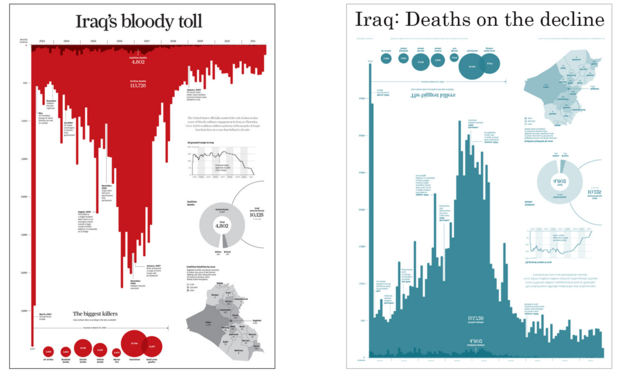
\includegraphics[width=1\linewidth]{./images/iraq-bloody-toll} 

}

\caption{Same data, two messages (Source: <a href="https://www.infoworld.com/article/3088166/why-how-to-lie-with-statistics-did-us-a-disservice.html">infoworld.com</a>)}\label{fig:img-dummy-coding}
\end{figure}

\hypertarget{further-resources}{%
\section{Further resources}\label{further-resources}}

\begin{itemize}
\tightlist
\item
  The \href{https://r-graphics.org/}{R Graphics Cookbook} by Winston Chang is available online with 150 ``recipes'' that cover everything from basic exploratory charts to colour-coded maps.
\item
  The BBC graphics team has published their own \href{https://bbc.github.io/rcookbook/}{R Cookbook} with many tips for making charts that convey a clear message, as well as some custom functions for making clean publication-ready charts.
\item
  Irizarry's \emph{Introduction to Data Science} has a good chapter on \href{https://rafalab.github.io/dsbook/data-visualization-principles.html}{data visualisation principles}
\end{itemize}

\hypertarget{part-quantitative-research}{%
\part*{Quantitative Research}\label{part-quantitative-research}}
\addcontentsline{toc}{part}{Quantitative Research}

\hypertarget{introduction}{%
\chapter{Introduction}\label{introduction}}

For an introduction to conducting and evaluating quantitative research, you can watch this video:

\hypertarget{key-concepts}{%
\section{Key concepts}\label{key-concepts}}

If you understand the following concepts, you will be in a good place to understand and assess quantitative research:

\begin{itemize}
\item
  \textbf{Hypothesis testing:} quantitative research aims to develop hypotheses and then check whether new data is consistent with these hypotheses. This sequence matters particularly for inferential statistics, i.e.~for knowing how to determine whether a certain pattern in the data is likely to arise due to random variation between samples we look at, or due to a real difference in the population of interest.
\item
  \textbf{Experiments with randomisation and blinding}. In essence, the idea is that if participants are randomly allocated to groups, the only difference between the groups is what happens during the experiment. If there is adequate blinding (i.e.~experimenters and participants do not know what condition they are assigned to), the only difference is that of interest (e.g., the content of a pill). Otherwise, experimenter and participant expectations will also differ, which might change results. You might want to have a look at this \href{https://s4be.cochrane.org/blog/2017/06/26/blinding-comprehensive-guide-students/}{detailed but brief discussion of blinding}
\item
  \textbf{Correlational/observational studies} and their inability to show causality: observational studies can be great to describe reality and to highlight associations, but without experiments (or more complex designs that aim to approximate experiments), we must be careful not to confuse correlation (co-occurrence of two variable) with causation (causal dependence of one on the other).
\item
  \textbf{Validity}

  \begin{itemize}
  \tightlist
  \item
    \textbf{Internal validity}: degree to which a study can rule out alternative explanations for the effects observed, apart from those highlighted by the researchers. This is most concerning in experimental research. A list of things that might reduce internal validity can be found \href{https://researchbasics.education.uconn.edu/experimental-_research/}{here}
  \item
    \textbf{External and ecological validity:} all about generalizability of results. External validity concerns generalisation to other participants, while ecological validity concerns the generalisation to real situations of interest. Detailed notes \href{https://researchbasics.education.uconn.edu/external_validity/\#}{here}
  \end{itemize}
\end{itemize}

\hypertarget{part-inferential-statistics}{%
\part*{Inferential statistics}\label{part-inferential-statistics}}
\addcontentsline{toc}{part}{Inferential statistics}

\hypertarget{simple-and-multiple-linear-regression}{%
\chapter{Simple and multiple linear regression}\label{simple-and-multiple-linear-regression}}

This document recaps how we assess relationships between variables when
at least the outcome variable is continuous.

\hypertarget{simple-linear-regression}{%
\section{Simple linear regression}\label{simple-linear-regression}}

For an introduction to simple linear regression and correlation, watch
this video:

When considering the relationship between two continuous variables, we
should always start with a scatterplot - for example, of the
relationship between social trust and life satisfaction at the national
level in European countries (data from the European Social Survey 2014).

\begin{Shaded}
\begin{Highlighting}[]
\NormalTok{pacman}\OperatorTok{::}\KeywordTok{p_load}\NormalTok{(tidyverse)}
\CommentTok{#Data preparation}
\NormalTok{ess <-}\StringTok{ }\KeywordTok{read_rds}\NormalTok{(}\KeywordTok{url}\NormalTok{(}\StringTok{"http://empower-training.de/Gold/round7.RDS"}\NormalTok{))}
\NormalTok{ess <-}\StringTok{ }\NormalTok{ess }\OperatorTok\StringTok{ }\KeywordTok{mutate}\NormalTok{(}\DataTypeTok{soctrust =}\NormalTok{ (ppltrst }\OperatorTok{+}\StringTok{ }\NormalTok{pplfair }\OperatorTok{+}\StringTok{ }\NormalTok{pplhlp)}\OperatorTok{/}\DecValTok{3}\NormalTok{)}
\NormalTok{nat_avgs <-}\StringTok{ }\NormalTok{ess }\OperatorTok\StringTok{ }\KeywordTok{group_by}\NormalTok{(cntry) }\OperatorTok\StringTok{ }
\StringTok{  }\KeywordTok{summarize}\NormalTok{(}\DataTypeTok{nat_soctrust =} \KeywordTok{mean}\NormalTok{(soctrust, }\DataTypeTok{na.rm=}\NormalTok{T), }
            \DataTypeTok{nat_stflife =} \KeywordTok{mean}\NormalTok{(stflife, }\DataTypeTok{na.rm=}\NormalTok{T))}

\KeywordTok{ggplot}\NormalTok{(nat_avgs, }\KeywordTok{aes}\NormalTok{(}\DataTypeTok{x=}\NormalTok{nat_soctrust, }\DataTypeTok{y=}\NormalTok{nat_stflife)) }\OperatorTok{+}\StringTok{ }\KeywordTok{geom_point}\NormalTok{()}
\end{Highlighting}
\end{Shaded}

\begin{figure}

{\centering \includegraphics[width=1\linewidth]{05-linear-regression_files/figure-latex/unnamed-chunk-1-1} 

}

\caption{Scatterplot relating social trust to life satisfaction}\label{fig:unnamed-chunk-1}
\end{figure}

The scatterplot can now help us to think about what kind of model would
help us to explain or predict one variable based on the other. If a
straight-line relationship seems reasonable, we can use a linear model.

\hypertarget{plotting-a-simple-linear-regression-model}{%
\subsection{Plotting a simple linear regression model}\label{plotting-a-simple-linear-regression-model}}

Geometrically, a simple linear regression model is just a straight line
through the scatterplot, fitted in a way that minimises the distances
from the points to the line. It can be plotted with the
\texttt{geom\_smooth(method="lm")} function.

\begin{Shaded}
\begin{Highlighting}[]
\KeywordTok{ggplot}\NormalTok{(nat_avgs, }\KeywordTok{aes}\NormalTok{(}\DataTypeTok{x=}\NormalTok{nat_soctrust, }\DataTypeTok{y=}\NormalTok{nat_stflife)) }\OperatorTok{+}\StringTok{ }
\StringTok{  }\KeywordTok{geom_point}\NormalTok{() }\OperatorTok{+}\StringTok{ }\KeywordTok{geom_smooth}\NormalTok{(}\DataTypeTok{method=}\StringTok{"lm"}\NormalTok{, }\DataTypeTok{se =} \OtherTok{FALSE}\NormalTok{) }
\end{Highlighting}
\end{Shaded}

\begin{figure}

{\centering 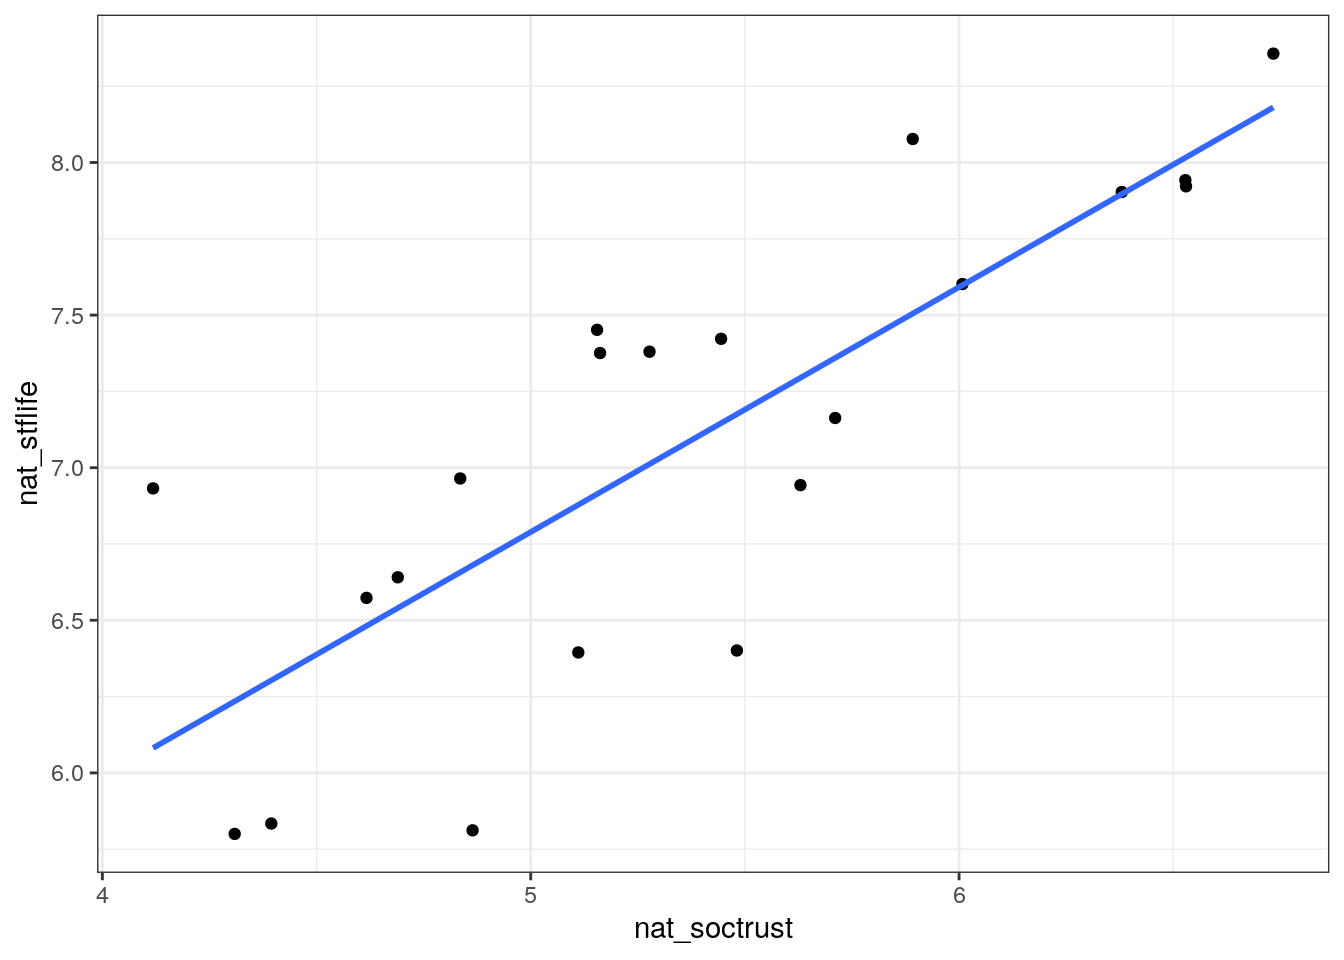
\includegraphics[width=1\linewidth]{05-linear-regression_files/figure-latex/unnamed-chunk-2-1} 

}

\caption{Scatterplot with added regression line ("line of best fit")}\label{fig:unnamed-chunk-2}
\end{figure}

\begin{Shaded}
\begin{Highlighting}[]
  \CommentTok{#se=FALSE hides confidence bands that are often just visual clutter}
\end{Highlighting}
\end{Shaded}

For each value of one variable, this line now allows us to find the
corresponding expected value of the other variable.

\hypertarget{mathematical-representation-of-a-simple-linear-regression-model}{%
\subsection{Mathematical representation of a simple linear regression model}\label{mathematical-representation-of-a-simple-linear-regression-model}}

The idea of a simple linear regression model is to link one predictor
variable, \(x\), to an outcome variable, \(y\). Their relationship can be
expressed in a simple formula: \[y=\beta_{0} +  \beta_{1}*x\] Here,
\(\beta_{1}\) is the most important parameter - it tells us, how much a
change of 1 in the \(x\)-variable affects the \(y\)-variable. Geometrically,
it is the slope of the regression line. \(\beta_{0}\) is the intercept of
that line, i.e.~the value of \(y\) when \(x\) is 0 - since \(x\) can often not
actually be zero, that parameter tends to be of little interest on its
own.

\hypertarget{fitting-a-simple-linear-regression-model-in-r}{%
\subsection{Fitting a simple linear regression model in R}\label{fitting-a-simple-linear-regression-model-in-r}}

Linear models are fitted in R using the \texttt{lm()} function. The model
itself is specified as a formula with the notation \texttt{y\ \textasciitilde{}\ x} where the \texttt{\textasciitilde{}}
means `is predicted by' and the intercept is added automatically.

\begin{Shaded}
\begin{Highlighting}[]
\KeywordTok{lm}\NormalTok{(nat_stflife }\OperatorTok{~}\StringTok{ }\NormalTok{nat_soctrust, }\DataTypeTok{data =}\NormalTok{ nat_avgs) }\OperatorTok\StringTok{ }\KeywordTok{summary}\NormalTok{()}
\end{Highlighting}
\end{Shaded}

\begin{verbatim}
## 
## Call:
## lm(formula = nat_stflife ~ nat_soctrust, data = nat_avgs)
## 
## Residuals:
##      Min       1Q   Median       3Q      Max 
## -0.86854 -0.35172  0.00667  0.30745  0.85047 
## 
## Coefficients:
##              Estimate Std. Error t value Pr(>|t|)    
## (Intercept)    2.7767     0.7311   3.798  0.00122 ** 
## nat_soctrust   0.8025     0.1347   5.957 9.84e-06 ***
## ---
## Signif. codes:  0 '***' 0.001 '**' 0.01 '*' 0.05 '.' 0.1 ' ' 1
## 
## Residual standard error: 0.4633 on 19 degrees of freedom
## Multiple R-squared:  0.6513,	Adjusted R-squared:  0.6329 
## F-statistic: 35.49 on 1 and 19 DF,  p-value: 9.839e-06
\end{verbatim}

In the summary, the first column of the coefficients table gives the
estimates for \(\beta_{0}\) (in the intercept row) and \(\beta_{1}\) (in the
nat\_soctrust row). Thus in this case, the regression formula could be
written as:

\[LifeSatisfaction = 2.76 +  0.80 * SocialTrust\] Clearly this formula
does not allow us to perfectly predict one variable from the other; we
have already seen in the graph that not all points fall exactly on the
line. The distances between each point and the line are the
\textbf{residuals} - their distribution is described at the top of the
\texttt{summary()}-function output.

\hypertarget{interpreting-r2}{%
\subsubsection{\texorpdfstring{Interpreting \(R^2\)}{Interpreting R\^{}2}}\label{interpreting-r2}}

The model output allows us to say how well the line fits by considering
the \(R^2\) value. It is based on the sum of the squares of the deviations
of each data point from either the mean (\(SS_{total}\)) or the model
(\(SS_{residual}\)).

If I was considering a model that predicted people's height, I might
have a person who is 1.6m tall. If the mean of the data was 1.8m, their
squared total deviation would be \(0.2*0.2 = 0.04\). If the model then
predicted their height at 1.55m, their squared residual deviation would
be \(-0.05*-0.05 = 0.025\). Once this is summed up for all data points,
\(R^2\) is calculated with the following formula:
\[R^2 = 1 - \frac{SS_{residual}}{SS_{total}}\]

Given that the sum of squared residuals can never be less than 0 or more
than the sum of the total residuals, \(R^2\) can only take up values
between 0 and 1. It can be understood as the share of total variance
explained by the model (or to link it to the formula: as the total
variance minus the share \emph{not} explained by the model).

\hypertarget{interpreting-prt-the-p-value}{%
\subsubsection{\texorpdfstring{Interpreting Pr(\textgreater\textbar t\textbar), the \emph{p}-value}{Interpreting Pr(\textgreater\textbar t\textbar), the p-value}}\label{interpreting-prt-the-p-value}}

Each coefficient comes with an associated \emph{p}-value in the summary that
is shown at the end of the row. As indicated by the column title, it
indicates the probability that the test statistic would be this large or
larger \emph{if} the null hypothesis was true and there was no association in
the underlying population.

As per usual, we would typically report coefficients with a \emph{p}-value
below .05 as statistically significant. The significance level for the
intercept is often not of interest - it simply indicates whether the
value of y is significantly different from 0 when x is 0.

There is also a \emph{p}-value for the overall model that essentially tests
whether \(R^2\) is significantly greater than 0. This is reported at the
very bottom of the \texttt{summary()}-output. If there is only one predictor
variable, this will the same as the \emph{p}-value for \(\beta_{1}\), but it
will be of greater interest when there are several predictors.

\hypertarget{bivariate-correlation}{%
\section{Bivariate correlation}\label{bivariate-correlation}}

Simple linear regression can tell us whether two variables are linearly
related to each other, whether this finding is statistically significant
(i.e.~clearer than what we might expect due to chance), and how strong
the relationship is \emph{in terms of the units of the two variables.} Quite
often, however, we would prefer a standardised measure of the strength
of a relationship, and a quicker test. That is where correlation comes
in.

The \textbf{Pearson's correlation coefficient} is the slope of the regression
line when both variables are standardised, i.e.~expressed in units of
their standard deviations (as so-called z-scores). It is again bounded,
between -1 and 1. As it is unit-free, it can give quick information as
to which relationships matter more and which matter less.

\hypertarget{calculating-the-correlation-coefficient}{%
\subsection{Calculating the correlation coefficient}\label{calculating-the-correlation-coefficient}}

Before calculating a correlation coefficient, \textbf{you need to look at the
scatterplot and make sure that a straight-line relationship looks
reasonable.} If that is the case, you can use the \texttt{cor.test()} function
to calculate the correlation coefficient.

\begin{Shaded}
\begin{Highlighting}[]
\KeywordTok{cor.test}\NormalTok{(nat_avgs}\OperatorTok{$}\NormalTok{nat_soctrust, nat_avgs}\OperatorTok{$}\NormalTok{nat_stflife) }
\CommentTok{#If you have missing data, use the na.rm = TRUE argument }
\CommentTok{#to have it excluded before the calculation}
\end{Highlighting}
\end{Shaded}

\begin{verbatim}
## 
## 	Pearson's product-moment correlation
## 
## data:  nat_avgs$nat_soctrust and nat_avgs$nat_stflife
## t = 5.957, df = 19, p-value = 9.839e-06
## alternative hypothesis: true correlation is not equal to 0
## 95 percent confidence interval:
##  0.5760041 0.9186640
## sample estimates:
##       cor 
## 0.8070221
\end{verbatim}

The estimated \texttt{cor} at the very bottom of the output is the correlation
coefficient, usually reported as \emph{r} = .81. This shows that there is a
strong positive relationship between the two variables. Check the
\emph{p}-value to see whether the relationship is statistically significant
and the 95\%-confidence interval to see how precise the estimate is
likely to be.

\hypertarget{equivalence-to-linear-regression}{%
\subsection{Equivalence to linear regression}\label{equivalence-to-linear-regression}}

Just to show that this is indeed equivalent to simple linear regression
on the standardised variables, which can be calculated using the
\texttt{scale()}-function.

\begin{Shaded}
\begin{Highlighting}[]
\KeywordTok{ggplot}\NormalTok{(nat_avgs, }\KeywordTok{aes}\NormalTok{(}\DataTypeTok{x=}\KeywordTok{scale}\NormalTok{(nat_soctrust), }\DataTypeTok{y=}\KeywordTok{scale}\NormalTok{(nat_stflife))) }\OperatorTok{+}\StringTok{ }
\StringTok{  }\KeywordTok{geom_point}\NormalTok{() }\OperatorTok{+}\StringTok{ }\KeywordTok{geom_smooth}\NormalTok{(}\DataTypeTok{method=}\StringTok{"lm"}\NormalTok{, }\DataTypeTok{se=}\OtherTok{FALSE}\NormalTok{) }\OperatorTok{+}\StringTok{ }\KeywordTok{labs}\NormalTok{(}\DataTypeTok{x=}\StringTok{"National Social Trust (standardised)"}\NormalTok{, }\DataTypeTok{y =} \StringTok{"National life satisfaction (standardised)"}\NormalTok{)}
\end{Highlighting}
\end{Shaded}

\begin{figure}

{\centering 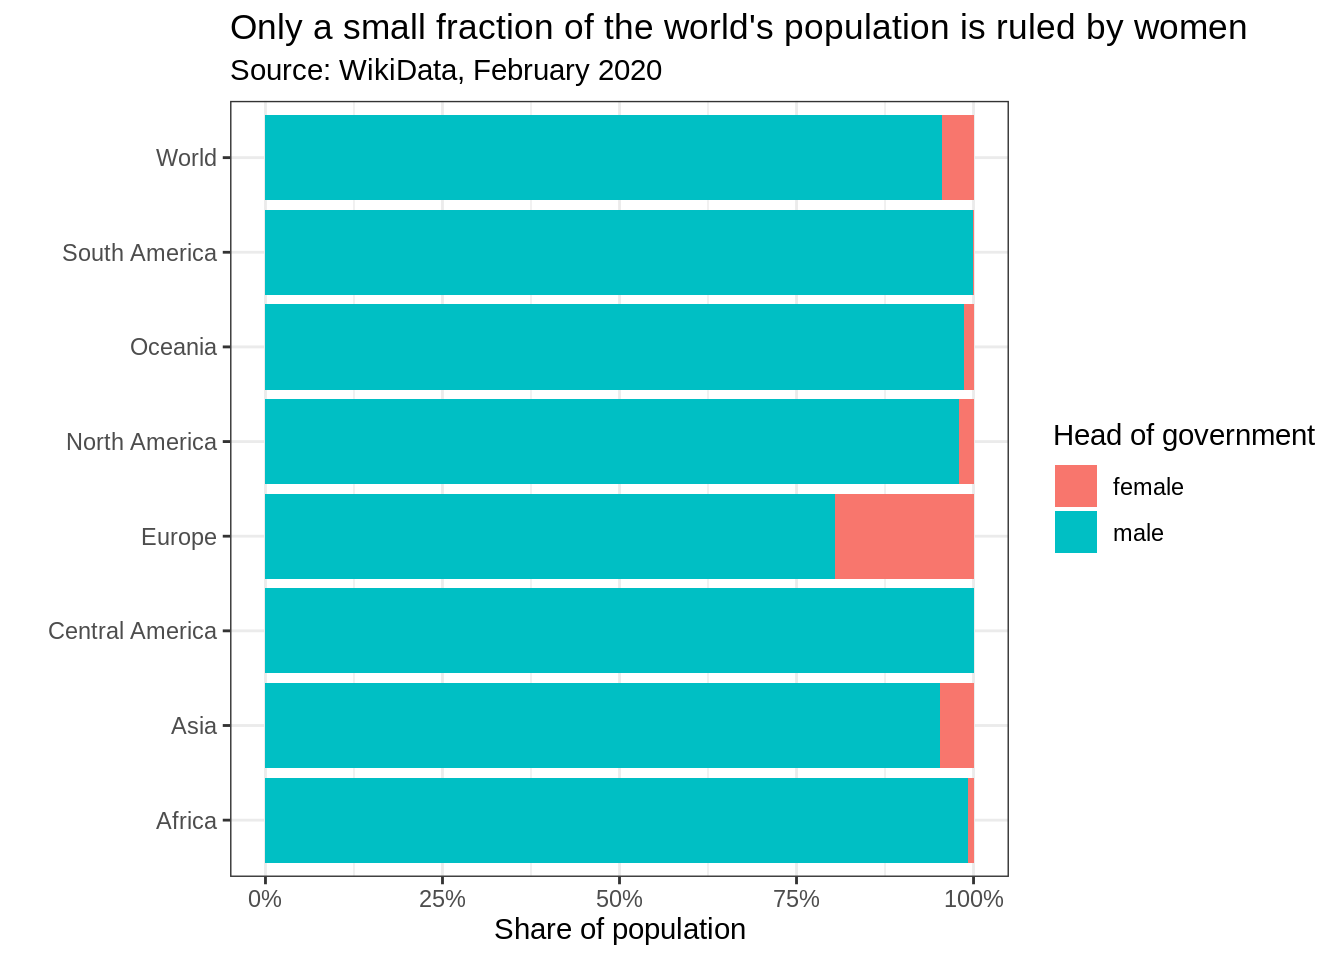
\includegraphics[width=1\linewidth]{05-linear-regression_files/figure-latex/unnamed-chunk-5-1} 

}

\caption{Scatterplot with scaled variables (z-scores)}\label{fig:unnamed-chunk-5}
\end{figure}

\begin{Shaded}
\begin{Highlighting}[]
\KeywordTok{lm}\NormalTok{(}\KeywordTok{scale}\NormalTok{(nat_stflife) }\OperatorTok{~}\StringTok{ }\KeywordTok{scale}\NormalTok{(nat_soctrust), }\DataTypeTok{data =}\NormalTok{ nat_avgs) }\OperatorTok\StringTok{ }\KeywordTok{summary}\NormalTok{()}
\end{Highlighting}
\end{Shaded}

\begin{verbatim}
## 
## Call:
## lm(formula = scale(nat_stflife) ~ scale(nat_soctrust), data = nat_avgs)
## 
## Residuals:
##      Min       1Q   Median       3Q      Max 
## -1.13572 -0.45992  0.00872  0.40203  1.11209 
## 
## Coefficients:
##                      Estimate Std. Error t value Pr(>|t|)    
## (Intercept)         1.910e-16  1.322e-01   0.000        1    
## scale(nat_soctrust) 8.070e-01  1.355e-01   5.957 9.84e-06 ***
## ---
## Signif. codes:  0 '***' 0.001 '**' 0.01 '*' 0.05 '.' 0.1 ' ' 1
## 
## Residual standard error: 0.6059 on 19 degrees of freedom
## Multiple R-squared:  0.6513,	Adjusted R-squared:  0.6329 
## F-statistic: 35.49 on 1 and 19 DF,  p-value: 9.839e-06
\end{verbatim}

Note that the regression coefficient for the scaled variable is
identical to the correlation coefficient shown above.

\hypertarget{multiple-linear-regression}{%
\section{Multiple linear regression}\label{multiple-linear-regression}}

Linear models can easily be extended to multiple predictor variables.
Here I will primarily focus on linear models that include categorical
predictor variables.

You can watch this video to take you through the process of extending
simple linear regression to include multiple variables step-by-step:

\hypertarget{dummy-coding-revisited}{%
\subsection{Dummy coding revisited}\label{dummy-coding-revisited}}

Multiple linear regression models often use categorical predictors.
However, they need to be turned into numbers. This is done through
automatic dummy coding, which creates variables coded as 0 and 1
(so-called dummy variables).

Note that dummy coding always results in \textbf{one fewer dummy variable than
the number of levels of the categorical variable}. For example, a
\emph{gender} variable with two levels (male/female) would be recoded into a
single dummy variable \emph{female} (0=no, 1=yes). Note that there is no
equivalent variable \emph{male} as that would be redundant. Given that the
hypothetical gender variable here is defined as either male or female,
not female necessarily implies male.

The same applies to larger number of levels - see below how three
possible values for the department variable would be recoded into two
dummy variables.

\begin{figure}

{\centering 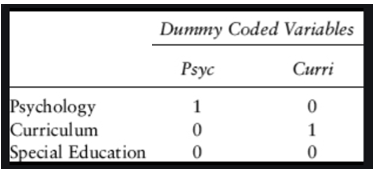
\includegraphics[width=1\linewidth]{./images/W10Dummy} 

}

\caption{Example for dummy-coding}\label{fig:img-dummy-coding}
\end{figure}

The level that is not explicitly mentioned anymore is the \textbf{reference
level} - in the case above, that is Special Education. In a linear
model, that is what all other effects are compared to, so it is
important to keep in mind which that is.

\hypertarget{mathematical-structure-of-multiple-linear-models}{%
\subsection{Mathematical structure of multiple linear models}\label{mathematical-structure-of-multiple-linear-models}}

Linear models are characterised by intercepts and slopes. Geometrically,
intercepts shift a line or plane along an axis, while a slope changes
its orientation in space. Conceptually, intercepts are like on/off
switches, while slopes indicate what happens when variables are dialed
up or down.

For example, we might want to predict life expectancy based on a
person's gender and their level of physical activity. Then the model
would be

\[LifeExpectancy=\beta_{0} +  \beta_{1}*female + \beta_{2}*activity\]
\(\beta_{0}\) here would describe the notional life expectancy of males
without any activity, \(\beta_{0}+\beta_{1}\) would describe that of
females without any exercise - so both of these are intercepts, the
\(female\) variable simply determines which intercept we choose.
\(\beta_{2}\) is now the effect of each unit of activity, i.e.~the slope
of the regression line.

\hypertarget{running-multiple-linear-regression-models-in-r}{%
\subsection{Running multiple linear regression models in R}\label{running-multiple-linear-regression-models-in-r}}

In the \texttt{lm()}-function, it is very easy to keep on adding predictors to
the formula by just using the \texttt{+}-symbol. For example, we can consider
the UK General Election Results in 2019 and see what helps explain the
vote share of the Conservatives.

\begin{Shaded}
\begin{Highlighting}[]
\CommentTok{#Load and prep data}
\NormalTok{constituencies <-}\StringTok{ }\KeywordTok{read_csv}\NormalTok{(}\KeywordTok{url}\NormalTok{(}\StringTok{"http://empower-training.de/Gold/ConstituencyData2019.csv"}\NormalTok{), }\DataTypeTok{col_types =} \StringTok{"_cfddddfffddddfffdfdddd"}\NormalTok{)}
\NormalTok{constituencies <-}\StringTok{ }\NormalTok{constituencies }\OperatorTok\StringTok{ }\KeywordTok{filter}\NormalTok{(RegionName }\OperatorTok{!=}\StringTok{ "Northern Ireland"}\NormalTok{) }\OperatorTok
\StringTok{          }\KeywordTok{mutate}\NormalTok{(}\DataTypeTok{nation =} \KeywordTok{case_when}\NormalTok{(RegionName }\OperatorTok{==}\StringTok{ "Scotland"} \OperatorTok{~}\StringTok{ "Scotland"}\NormalTok{,}
\NormalTok{                                    RegionName }\OperatorTok{==}\StringTok{ "Wales"} \OperatorTok{~}\StringTok{ "Wales"}\NormalTok{,}
\NormalTok{                                    T }\OperatorTok{~}\StringTok{ "England"}\NormalTok{))  }\OperatorTok\StringTok{ }
\StringTok{          }\KeywordTok{filter}\NormalTok{(ConstituencyName }\OperatorTok{!=}\StringTok{ "Chorley"}\NormalTok{)}

\CommentTok{#Simple linear regression model:}
\KeywordTok{lm}\NormalTok{(ElectionConShare }\OperatorTok{~}\StringTok{ }\NormalTok{MedianAge, }\DataTypeTok{data =}\NormalTok{ constituencies) }\OperatorTok\StringTok{ }\KeywordTok{summary}\NormalTok{()}
\end{Highlighting}
\end{Shaded}

\begin{verbatim}
## 
## Call:
## lm(formula = ElectionConShare ~ MedianAge, data = constituencies)
## 
## Residuals:
##      Min       1Q   Median       3Q      Max 
## -0.41131 -0.09130  0.01502  0.10007  0.30207 
## 
## Coefficients:
##              Estimate Std. Error t value Pr(>|t|)    
## (Intercept) -0.252020   0.040956  -6.153 1.35e-09 ***
## MedianAge    0.017104   0.001003  17.054  < 2e-16 ***
## ---
## Signif. codes:  0 '***' 0.001 '**' 0.01 '*' 0.05 '.' 0.1 ' ' 1
## 
## Residual standard error: 0.1384 on 629 degrees of freedom
## Multiple R-squared:  0.3162,	Adjusted R-squared:  0.3151 
## F-statistic: 290.8 on 1 and 629 DF,  p-value: < 2.2e-16
\end{verbatim}

We now know that the Conservative vote share seems to be strongly
related to the median age of the constituency, and can find and
interpret the coefficient estimate (1.7 pct-points per year of median
age), significance value and \(R^2\) as above. What happens when we add
nation, to account for differences between Scotland, England and Wales?

\begin{Shaded}
\begin{Highlighting}[]
\CommentTok{#Declare nation as factor and then set the reference level }
\CommentTok{#for categorical predictors}
\NormalTok{constituencies}\OperatorTok{$}\NormalTok{nation <-}\StringTok{ }\KeywordTok{factor}\NormalTok{(constituencies}\OperatorTok{$}\NormalTok{nation) }\OperatorTok\StringTok{ }\KeywordTok{relevel}\NormalTok{(}\DataTypeTok{ref =} \StringTok{"England"}\NormalTok{)}
\KeywordTok{lm}\NormalTok{(ElectionConShare }\OperatorTok{~}\StringTok{ }\NormalTok{MedianAge }\OperatorTok{+}\StringTok{ }\NormalTok{nation, }\DataTypeTok{data =}\NormalTok{ constituencies) }\OperatorTok\StringTok{ }\KeywordTok{summary}\NormalTok{()}
\end{Highlighting}
\end{Shaded}

\begin{verbatim}
## 
## Call:
## lm(formula = ElectionConShare ~ MedianAge + nation, data = constituencies)
## 
## Residuals:
##      Min       1Q   Median       3Q      Max 
## -0.37287 -0.06969  0.00687  0.07799  0.27545 
## 
## Coefficients:
##                  Estimate Std. Error t value Pr(>|t|)    
## (Intercept)    -0.2777133  0.0337157  -8.237 1.03e-15 ***
## MedianAge       0.0185574  0.0008295  22.373  < 2e-16 ***
## nationScotland -0.2527752  0.0156649 -16.136  < 2e-16 ***
## nationWales    -0.1493447  0.0187193  -7.978 7.08e-15 ***
## ---
## Signif. codes:  0 '***' 0.001 '**' 0.01 '*' 0.05 '.' 0.1 ' ' 1
## 
## Residual standard error: 0.1138 on 627 degrees of freedom
## Multiple R-squared:  0.5392,	Adjusted R-squared:  0.537 
## F-statistic: 244.6 on 3 and 627 DF,  p-value: < 2.2e-16
\end{verbatim}

Now we have a more complex model. Based on the coefficient estimates, we
would now estimate the vote share as follows
\[VoteShare=-0.27 +  0.018*age + -0.25*Scotland + -0.15*Wales\] The
figures for Scotland and Wales need to be compared to the unnamed
reference level, i.e.~to England - so we would expect a Scottish
constituency to have a 25 percentage points lower Conservative vote
share \emph{when keeping median age constant.} Likewise, we now would expect
an increase of the median age by 1 year to increase the Conservative
vote share by 1.8 percentage points, \emph{keeping the effect of nation
constant.}

\begin{Shaded}
\begin{Highlighting}[]
\CommentTok{#The moderndive is needed to plot parallel regression lines}
\NormalTok{pacman}\OperatorTok{::}\KeywordTok{p_load}\NormalTok{(}\StringTok{"moderndive"}\NormalTok{)}

\KeywordTok{ggplot}\NormalTok{(constituencies, }\KeywordTok{aes}\NormalTok{(}\DataTypeTok{x=}\NormalTok{MedianAge, }\DataTypeTok{y=}\NormalTok{ElectionConShare, }\DataTypeTok{color =}\NormalTok{ nation)) }\OperatorTok{+}\StringTok{ }\KeywordTok{geom_point}\NormalTok{() }\OperatorTok{+}\StringTok{ }\NormalTok{moderndive}\OperatorTok{::}\KeywordTok{geom_parallel_slopes}\NormalTok{(}\DataTypeTok{se =} \OtherTok{FALSE}\NormalTok{)}
\end{Highlighting}
\end{Shaded}

\begin{figure}

{\centering \includegraphics[width=1\linewidth]{05-linear-regression_files/figure-latex/unnamed-chunk-8-1} 

}

\caption{Multiple regression model to predict Tory 2019 vote share}\label{fig:unnamed-chunk-8}
\end{figure}

\hypertarget{significance-testing-and-reporting-in-multiple-regression-models}{%
\subsubsection{Significance testing and reporting in multiple regression models}\label{significance-testing-and-reporting-in-multiple-regression-models}}

With more than one predictor, we have two questions:

\begin{itemize}
\tightlist
\item
  is the \textbf{overall model} significant, i.e.~can we confidently
  believe that its estimates are better than if we just took the
  overall mean as our estimate for each constituency? That is shown in
  the last line of the summary. Here we would report that the
  regression model predicting the conservative vote share per
  constituency based on its median age and the nation it was located
  in was significant, with \emph{F}(3, 627) = 244.6, \emph{p} \textless{} .001, and
  explained a substantial share of the variance, \(R^2\) = .54.
\item
  does \textbf{each predictor} explain a significant share of unique
  variance? That is shown at the end of each line in the coefficients
  table. With many predictors, coefficients and significance levels
  would usually be reported in a table.
\end{itemize}

\hypertarget{comparing-means-between-conditions-or-groups}{%
\chapter{Comparing means between conditions or groups}\label{comparing-means-between-conditions-or-groups}}

Watch this video for an introduction to testing for differences between two means and the differences between repeated measures and independent samples:

Watch this video for an introduction to testing for differences between \emph{more than} two means:

\hypertarget{repeated-measures-or-independent-samples}{%
\subsection{Repeated measures or independent samples}\label{repeated-measures-or-independent-samples}}

The first question always needs to be whether each participant contributes one or several data points to the dependent variable that is compared. If they contribute only one, we have an \emph{independent samples} or \emph{between-participants} design; if they contribute several, the design is \emph{repeated measures} or \emph{within participants.} In the latter case, we need to account for the relationships between some of the measurements in our analysis.

\hypertarget{two-independent-means}{%
\subsection{Two independent means}\label{two-independent-means}}

Going back to the European Social Survey 2014 data, we might be curious whether social trust differs between men and women in the UK. For that, we should always first calculate the descriptive statistics:

\begin{Shaded}
\begin{Highlighting}[]
\NormalTok{pacman}\OperatorTok{::}\KeywordTok{p_load}\NormalTok{(tidyverse)}
\NormalTok{ess <-}\StringTok{ }\KeywordTok{read_rds}\NormalTok{(}\KeywordTok{url}\NormalTok{(}\StringTok{"http://empower-training.de/Gold/round7.RDS"}\NormalTok{))}
\NormalTok{ess <-}\StringTok{ }\NormalTok{ess }\OperatorTok\StringTok{ }\KeywordTok{mutate}\NormalTok{(}\DataTypeTok{soctrust =}\NormalTok{ (ppltrst }\OperatorTok{+}\StringTok{ }\NormalTok{pplfair }\OperatorTok{+}\StringTok{ }\NormalTok{pplhlp)}\OperatorTok{/}\DecValTok{3}\NormalTok{)}
\NormalTok{essUK <-}\StringTok{ }\NormalTok{ess }\OperatorTok\StringTok{ }\KeywordTok{filter}\NormalTok{(cntry}\OperatorTok{==}\StringTok{"GB"}\NormalTok{)}
\NormalTok{essUK }\OperatorTok\StringTok{ }\KeywordTok{group_by}\NormalTok{(gndr) }\OperatorTok\StringTok{ }\KeywordTok{summarise}\NormalTok{(}\KeywordTok{mean}\NormalTok{(soctrust, }\DataTypeTok{na.rm =} \OtherTok{TRUE}\NormalTok{))}
\end{Highlighting}
\end{Shaded}

\begin{verbatim}
## # A tibble: 2 x 2
##   gndr   `mean(soctrust, na.rm = TRUE)`
## * <fct>                           <dbl>
## 1 Male                             5.70
## 2 Female                           5.72
\end{verbatim}

Those means look very close. Nevertheless, we might want to know how likely we would have been to see a difference this large under the null-hypothesis, i.e.~if social trust did not differ between men and women. For that, we can run a t-test.

\begin{Shaded}
\begin{Highlighting}[]
\KeywordTok{t.test}\NormalTok{(soctrust }\OperatorTok{~}\StringTok{ }\NormalTok{gndr, }\DataTypeTok{data=}\NormalTok{essUK, }\DataTypeTok{var.equal =} \OtherTok{TRUE}\NormalTok{)}
\end{Highlighting}
\end{Shaded}

\begin{verbatim}
## 
## 	Two Sample t-test
## 
## data:  soctrust by gndr
## t = -0.2116, df = 2248, p-value = 0.8324
## alternative hypothesis: true difference in means is not equal to 0
## 95 percent confidence interval:
##  -0.1601569  0.1289597
## sample estimates:
##   mean in group Male mean in group Female 
##             5.702288             5.717886
\end{verbatim}

This is just a special case of a linear model, so we could also use the \texttt{lm()} function:

\begin{Shaded}
\begin{Highlighting}[]
\KeywordTok{lm}\NormalTok{(soctrust }\OperatorTok{~}\StringTok{ }\NormalTok{gndr, }\DataTypeTok{data=}\NormalTok{essUK) }\OperatorTok\StringTok{ }\KeywordTok{summary}\NormalTok{()}
\end{Highlighting}
\end{Shaded}

\begin{verbatim}
## 
## Call:
## lm(formula = soctrust ~ gndr, data = essUK)
## 
## Residuals:
##     Min      1Q  Median      3Q     Max 
## -5.7179 -1.0512  0.2821  1.2821  4.2977 
## 
## Coefficients:
##             Estimate Std. Error t value Pr(>|t|)    
## (Intercept)  5.70229    0.05450 104.623   <2e-16 ***
## gndrFemale   0.01560    0.07372   0.212    0.832    
## ---
## Signif. codes:  0 '***' 0.001 '**' 0.01 '*' 0.05 '.' 0.1 ' ' 1
## 
## Residual standard error: 1.741 on 2248 degrees of freedom
##   (14 observations deleted due to missingness)
## Multiple R-squared:  1.992e-05,	Adjusted R-squared:  -0.0004249 
## F-statistic: 0.04478 on 1 and 2248 DF,  p-value: 0.8324
\end{verbatim}

Both show, as expected, that the difference we observed could easily have been due to chance, and show the same \emph{p} and \emph{t}-values. You might report this by saying: there was no significant difference in social trust between men and women, \emph{t}(2248) = -0.21, \emph{p} = .83.

\hypertarget{two-dependent-means}{%
\subsection{Two dependent means}\label{two-dependent-means}}

In the ESS data, participants were asked how much they drank when they last drank during a weekday and during a weekend. Here the same participants provided two alcohol measures, so that these data points represent repeated measures. If we ignore that in the analysis, we violate a key assumption of linear models - namely the independence of observations. Therefore, we need to use a paired t-test. But as always, first descriptive statistics.

\begin{Shaded}
\begin{Highlighting}[]
\NormalTok{essUK }\OperatorTok\StringTok{ }
\StringTok{  }\KeywordTok{summarise}\NormalTok{(}\DataTypeTok{weekday =} \KeywordTok{mean}\NormalTok{(alcwkdy, }\DataTypeTok{na.rm=}\NormalTok{T), }\DataTypeTok{weekend=}\KeywordTok{mean}\NormalTok{(alcwknd, }\DataTypeTok{na.rm =}\NormalTok{ T)) }\OperatorTok
\StringTok{  }\KeywordTok{mutate}\NormalTok{(}\DataTypeTok{diff =}\NormalTok{ weekend }\OperatorTok{-}\StringTok{ }\NormalTok{weekday)}
\end{Highlighting}
\end{Shaded}

\begin{verbatim}
## # A tibble: 1 x 3
##   weekday weekend  diff
##     <dbl>   <dbl> <dbl>
## 1    36.3    62.4  26.1
\end{verbatim}

So there seems to be a large difference in the average amount people drink during a single session on weekdays and weekends. Is the difference statistically significant?

\begin{Shaded}
\begin{Highlighting}[]
\KeywordTok{t.test}\NormalTok{(essUK}\OperatorTok{$}\NormalTok{alcwknd, essUK}\OperatorTok{$}\NormalTok{alcwkdy, }\DataTypeTok{paired =} \OtherTok{TRUE}\NormalTok{)}
\end{Highlighting}
\end{Shaded}

\begin{verbatim}
## 
## 	Paired t-test
## 
## data:  essUK$alcwknd and essUK$alcwkdy
## t = 13.119, df = 1800, p-value < 2.2e-16
## alternative hypothesis: true difference in means is not equal to 0
## 95 percent confidence interval:
##  22.23332 30.04986
## sample estimates:
## mean of the differences 
##                26.14159
\end{verbatim}

The paired t-test - as it says in the output - tests whether the mean of the differences between the two variables is significantly different from 0. We could also specify that condition directly to receive identical results :

\begin{Shaded}
\begin{Highlighting}[]
\KeywordTok{t.test}\NormalTok{(essUK}\OperatorTok{$}\NormalTok{alcwknd }\OperatorTok{-}\StringTok{ }\NormalTok{essUK}\OperatorTok{$}\NormalTok{alcwkdy, }\DataTypeTok{mu =} \DecValTok{0}\NormalTok{)}
\end{Highlighting}
\end{Shaded}

\begin{verbatim}
## 
## 	One Sample t-test
## 
## data:  essUK$alcwknd - essUK$alcwkdy
## t = 13.119, df = 1800, p-value < 2.2e-16
## alternative hypothesis: true mean is not equal to 0
## 95 percent confidence interval:
##  22.23332 30.04986
## sample estimates:
## mean of x 
##  26.14159
\end{verbatim}

\hypertarget{more-than-two-independent-means}{%
\subsection{More than two independent means}\label{more-than-two-independent-means}}

We might be interested whether levels of life satisfaction differ between the European countries we could reach by ferry from the UK. First, let's look at the descriptive statistics.

\begin{Shaded}
\begin{Highlighting}[]
\NormalTok{essF <-}\StringTok{ }\NormalTok{ess }\OperatorTok\StringTok{ }\KeywordTok{filter}\NormalTok{(cntry }\OperatorTok\StringTok{ }\KeywordTok{c}\NormalTok{(}\StringTok{"FR"}\NormalTok{, }\StringTok{"ES"}\NormalTok{, }\StringTok{"IE"}\NormalTok{, }\StringTok{"BE"}\NormalTok{, }\StringTok{"NL"}\NormalTok{))}
\NormalTok{essF }\OperatorTok\StringTok{ }\KeywordTok{group_by}\NormalTok{(cntry) }\OperatorTok\StringTok{ }\KeywordTok{summarise}\NormalTok{(}\DataTypeTok{life_satisfaction =} \KeywordTok{mean}\NormalTok{(stflife, }\DataTypeTok{na.rm =}\NormalTok{ T))}
\end{Highlighting}
\end{Shaded}

\begin{verbatim}
## # A tibble: 5 x 2
##   cntry life_satisfaction
## * <fct>             <dbl>
## 1 BE                 7.45
## 2 ES                 6.96
## 3 FR                 6.39
## 4 IE                 6.94
## 5 NL                 7.60
\end{verbatim}

There seem to be some differences - but are they statistically significant? Here we actually have two questions:

\begin{itemize}
\tightlist
\item
  do the countries together explain a significant share of the variance in life satisfaction? (\emph{omnibus test})
\item
  are the levels of life satisfaction in any two countries significantly different from each other? (\emph{pairwise comparisons})
\end{itemize}

\hypertarget{omnibus-test-anova}{%
\subsubsection{Omnibus test (ANOVA)}\label{omnibus-test-anova}}

\begin{Shaded}
\begin{Highlighting}[]
\CommentTok{#Set the reference level, so that we know what the coefficients mean}
\NormalTok{essF}\OperatorTok{$}\NormalTok{cntry <-}\StringTok{ }\KeywordTok{factor}\NormalTok{(essF}\OperatorTok{$}\NormalTok{cntry) }\OperatorTok\StringTok{ }\KeywordTok{relevel}\NormalTok{(}\DataTypeTok{ref =} \StringTok{"FR"}\NormalTok{)}
\KeywordTok{lm}\NormalTok{(stflife }\OperatorTok{~}\StringTok{ }\NormalTok{cntry, }\DataTypeTok{data =}\NormalTok{ essF) }\OperatorTok\StringTok{ }\KeywordTok{summary}\NormalTok{()}
\end{Highlighting}
\end{Shaded}

\begin{verbatim}
## 
## Call:
## lm(formula = stflife ~ cntry, data = essF)
## 
## Residuals:
##     Min      1Q  Median      3Q     Max 
## -7.6017 -0.9646  0.3983  1.3983  3.6054 
## 
## Coefficients:
##             Estimate Std. Error t value Pr(>|t|)    
## (Intercept)  6.39456    0.04612 138.663   <2e-16 ***
## cntryBE      1.05711    0.06651  15.893   <2e-16 ***
## cntryES      0.57006    0.06512   8.753   <2e-16 ***
## cntryIE      0.54832    0.06192   8.856   <2e-16 ***
## cntryNL      1.20711    0.06516  18.526   <2e-16 ***
## ---
## Signif. codes:  0 '***' 0.001 '**' 0.01 '*' 0.05 '.' 0.1 ' ' 1
## 
## Residual standard error: 2.016 on 9896 degrees of freedom
##   (19 observations deleted due to missingness)
## Multiple R-squared:  0.04125,	Adjusted R-squared:  0.04086 
## F-statistic: 106.4 on 4 and 9896 DF,  p-value: < 2.2e-16
\end{verbatim}

Here we just want to see whether the country variable explains a significant share of the variance. That is shown by the last line, so that we would report: There was an overall effects of country on life satisfaction, \emph{F}(4, 9869) = 106.4, \emph{p}\textless.001.

If you are so inclined, note that this is identical to a one-way ANOVA. To see that, you can replace summary() by car::Anova() - however, this is only truly essential if you are a psychologist, most other disciplines prefer the plain linear models when they suffice.

\begin{Shaded}
\begin{Highlighting}[]
\NormalTok{pacman}\OperatorTok{::}\KeywordTok{p_load}\NormalTok{(car)}
\end{Highlighting}
\end{Shaded}

\begin{verbatim}
## Installing package into '/home/runner/work/_temp/Library'
## (as 'lib' is unspecified)
\end{verbatim}

\begin{verbatim}
## also installing the dependencies 'matrixStats', 'RcppArmadillo', 'zip', 'numDeriv', 'SparseM', 'MatrixModels', 'conquer', 'sp', 'data.table', 'openxlsx', 'minqa', 'nloptr', 'statmod', 'RcppEigen', 'carData', 'abind', 'pbkrtest', 'quantreg', 'maptools', 'rio', 'lme4'
\end{verbatim}

\begin{verbatim}
## 
## car installed
\end{verbatim}

\begin{Shaded}
\begin{Highlighting}[]
\KeywordTok{lm}\NormalTok{(stflife }\OperatorTok{~}\StringTok{ }\NormalTok{cntry, }\DataTypeTok{data =}\NormalTok{ essF) }\OperatorTok\StringTok{ }\NormalTok{car}\OperatorTok{::}\KeywordTok{Anova}\NormalTok{()}
\end{Highlighting}
\end{Shaded}

\begin{verbatim}
## Anova Table (Type II tests)
## 
## Response: stflife
##           Sum Sq   Df F value    Pr(>F)    
## cntry       1730    4  106.45 < 2.2e-16 ***
## Residuals  40218 9896                      
## ---
## Signif. codes:  0 '***' 0.001 '**' 0.01 '*' 0.05 '.' 0.1 ' ' 1
\end{verbatim}

\hypertarget{pairwise-comparisons}{%
\subsubsection{Pairwise comparisons}\label{pairwise-comparisons}}

Now that we know that some of the countries are different, we will want to locate the differences. That is where pairwise t-tests come in.

\begin{Shaded}
\begin{Highlighting}[]
\KeywordTok{pairwise.t.test}\NormalTok{(essF}\OperatorTok{$}\NormalTok{stflife, essF}\OperatorTok{$}\NormalTok{cntry, }\DataTypeTok{p.adjust.method =} \StringTok{"bonferroni"}\NormalTok{)}
\end{Highlighting}
\end{Shaded}

\begin{verbatim}
## 
## 	Pairwise comparisons using t tests with pooled SD 
## 
## data:  essF$stflife and essF$cntry 
## 
##    FR      BE      ES      IE     
## BE < 2e-16 -       -       -      
## ES < 2e-16 2.4e-12 -       -      
## IE < 2e-16 1.0e-14 1.00    -      
## NL < 2e-16 0.24    < 2e-16 < 2e-16
## 
## P value adjustment method: bonferroni
\end{verbatim}

This gives us \emph{p}-values for all tests, that are adjusted for the fact that we are doing many (i.e.~10) comparisons and thus running a greater risk of getting a false positive. The Bonferroni adjustment, selected here, multiplies each \emph{p}-value by the number of comparisons, unless the resulting value would exceed 1 and thus be an impossible probability.

Combining this with the descriptive statistics, we can say, for instance, that the people in the Netherlands and Belgium are more satisfied with life than those in any of the other countries, but that their satisfaction levels do not differ significantly from each other.

\hypertarget{more-than-two-means-from-repeated-measures}{%
\subsection{More than two means from repeated measures}\label{more-than-two-means-from-repeated-measures}}

Here I will revert to the simulated example from the video linked above. In that, the effect of four conditions during studying on participants' test scores was assessed, namely whether participants were exposed to instrumental music, vocal music, white noise or silence.

Note that the data for repeated measures analysis in R generally needs to be formatted in a way that each row shows one observation rather than multiple observations from one participant (``long'' format). If you have data in a ``wide'' format, you can reshape it with the \texttt{gather()} or \texttt{pivot\_longer()} functions.

To analyse whether there are differences between the conditions, as always, we start with descriptive statistics.

\begin{Shaded}
\begin{Highlighting}[]
\NormalTok{noiseData }\OperatorTok\StringTok{ }\KeywordTok{group_by}\NormalTok{(condition) }\OperatorTok\StringTok{ }\KeywordTok{summarise}\NormalTok{(}\KeywordTok{mean}\NormalTok{(score))}
\end{Highlighting}
\end{Shaded}

\begin{verbatim}
## # A tibble: 4 x 2
##   condition    `mean(score)`
## * <chr>                <dbl>
## 1 instrumental          11.6
## 2 silence               13.0
## 3 vocals                10.8
## 4 whiteNoise            13.5
\end{verbatim}

It looks like there are some differences, but to be able to judge statistical significance, we would again be interested in omnibus tests and then pairwise comparisons.

\hypertarget{omnibus-test}{%
\subsubsection{Omnibus test}\label{omnibus-test}}

Testing whether the conditions make a difference is a little bit harder with repeated measures because the observations are not independent. Therefore, we need to run a model that takes into account the relationships between the observations taken from a single participant. This does not work with \texttt{lm()}; instead we need to use an additional package that allows for multi-level modeling where some observations are clustered together, \texttt{lme4} is the most frequently used such package for this purpose.

In the case of independent samples, we were comparing our model with the group variable as a predictor implicitly to the model that predicts the overall mean for everyone (that is what the \texttt{lm()} F-test is doing). Here, the null model uses each participant's own overall mean as the prediction for their performance in any one condition. We need to set up that null model explicitly and then compare it to the model that considers groups.

\begin{Shaded}
\begin{Highlighting}[]
\NormalTok{pacman}\OperatorTok{::}\KeywordTok{p_load}\NormalTok{(lme4)}

\CommentTok{#Set reference level explicitly}
\NormalTok{noiseData}\OperatorTok{$}\NormalTok{condition <-}\StringTok{ }\NormalTok{noiseData}\OperatorTok{$}\NormalTok{condition }\OperatorTok\StringTok{ }\KeywordTok{factor}\NormalTok{() }\OperatorTok\StringTok{ }\KeywordTok{relevel}\NormalTok{(}\StringTok{"silence"}\NormalTok{)}

\CommentTok{#Run null model - predicting only an individual intercept per participant}
\NormalTok{model0 <-}\StringTok{ }\KeywordTok{lmer}\NormalTok{((score }\OperatorTok{~}\StringTok{ }\NormalTok{(}\DecValTok{1} \OperatorTok{|}\StringTok{ }\NormalTok{participantID)),	}\DataTypeTok{data =}\NormalTok{ noiseData)}

\CommentTok{#Run hypothesized model - adding the groups as a predictor}
\NormalTok{model1 <-}\StringTok{ }\KeywordTok{lmer}\NormalTok{((score }\OperatorTok{~}\StringTok{ }\NormalTok{condition }\OperatorTok{+}\StringTok{ }\NormalTok{(}\DecValTok{1} \OperatorTok{|}\StringTok{ }\NormalTok{participantID)),	}\DataTypeTok{data =}\NormalTok{ noiseData)}

\CommentTok{#Comparing the two models}
\KeywordTok{anova}\NormalTok{(model0, model1)}
\end{Highlighting}
\end{Shaded}

\begin{verbatim}
## refitting model(s) with ML (instead of REML)
\end{verbatim}

\begin{verbatim}
## Data: noiseData
## Models:
## model0: score ~ (1 | participantID)
## model1: score ~ condition + (1 | participantID)
##        npar    AIC    BIC  logLik deviance  Chisq Df Pr(>Chisq)    
## model0    3 480.29 488.10 -237.14   474.29                         
## model1    6 447.31 462.94 -217.66   435.31 38.978  3  1.754e-08 ***
## ---
## Signif. codes:  0 '***' 0.001 '**' 0.01 '*' 0.05 '.' 0.1 ' ' 1
\end{verbatim}

Here we can see that the hypothesised model showed a significantly better fit. This is tested with a \(\chi^2\)-test, which we will look at further later in the course, but the key criterion again is that \emph{p} (here Pr(\textgreater Chisq)) is smaller than .05.

\hypertarget{pairwise-comparisons-1}{%
\subsubsection{Pairwise comparisons}\label{pairwise-comparisons-1}}

Now that we know that there is a difference between some of the conditions, we will want to know which are different. For that, we can again run pairwise t-tests; we just need to specify that they are run on paired data by setting \texttt{paired\ =\ TRUE}.

\begin{Shaded}
\begin{Highlighting}[]
\KeywordTok{pairwise.t.test}\NormalTok{(noiseData}\OperatorTok{$}\NormalTok{score, noiseData}\OperatorTok{$}\NormalTok{condition,	}\DataTypeTok{p.adj =} \StringTok{"bonferroni"}\NormalTok{, }\DataTypeTok{paired=}\OtherTok{TRUE}\NormalTok{)}
\end{Highlighting}
\end{Shaded}

\begin{verbatim}
## 
## 	Pairwise comparisons using paired t tests 
## 
## data:  noiseData$score and noiseData$condition 
## 
##              silence instrumental vocals 
## instrumental 0.045   -            -      
## vocals       8.2e-06 0.423        -      
## whiteNoise   1.000   0.001        2.0e-05
## 
## P value adjustment method: bonferroni
\end{verbatim}

This indicates that the scores of participants in the white noise and silence conditions were not significantly different from each other, nor were those between vocals and instrumental music. Only the four comparisons between `music' and `non-music' conditions were significant.

\hypertarget{interaction-terms-in-linear-models}{%
\chapter{Interaction terms in linear models}\label{interaction-terms-in-linear-models}}

Watch this video for an introduction to interaction terms in linear models:

The section below essentially contains the code needed for the examples in the video, with some further annotations. Before that, just one note on terminology:

\begin{itemize}
\tightlist
\item
  Generally, if two variables interact, then the effect that one has on the predictor (the regression slope) depends on the value of the other. Mathematically, that relationship is symetrical - if A interacts with B, then B interacts with A.
\item
  For interpretation, we often designate one of the variables as the \emph{moderator}. That just means that we are primarily interested in the effect of the other variable on the outcome and in how the moderator changes that effect. Often, demographic variables such as age or gender serve as moderators.
\end{itemize}

\hypertarget{example-1-memory-and-chess}{%
\section{Example 1: Memory and chess}\label{example-1-memory-and-chess}}

The first example draws on research by Gobet \& Simon (1996) but uses simulated data.

Show the code to simulate the data

\begin{Shaded}
\begin{Highlighting}[]
\KeywordTok{library}\NormalTok{(tidyverse)}

\CommentTok{#Generate data (errors committed) - *roughly* based on Gobet & Simon 1996}
\KeywordTok{set.seed}\NormalTok{(}\DecValTok{300688}\NormalTok{) }\CommentTok{#for reproducible results}
\NormalTok{ER <-}\StringTok{ }\KeywordTok{rnorm}\NormalTok{(}\DecValTok{50}\NormalTok{, }\FloatTok{4.9}\NormalTok{,}\FloatTok{3.5}\NormalTok{) }\OperatorTok{+}\StringTok{ }\KeywordTok{rnorm}\NormalTok{(}\DecValTok{50}\NormalTok{, }\DecValTok{0}\NormalTok{, }\DecValTok{2}\NormalTok{)}
\NormalTok{NR <-}\StringTok{ }\KeywordTok{rnorm}\NormalTok{(}\DecValTok{50}\NormalTok{, }\FloatTok{15.7}\NormalTok{, }\FloatTok{4.0}\NormalTok{) }\OperatorTok{+}\StringTok{ }\KeywordTok{rnorm}\NormalTok{(}\DecValTok{50}\NormalTok{, }\DecValTok{0}\NormalTok{, }\DecValTok{2}\NormalTok{)}
\NormalTok{EF <-}\StringTok{ }\KeywordTok{rnorm}\NormalTok{(}\DecValTok{50}\NormalTok{, }\FloatTok{21.4}\NormalTok{, }\DecValTok{5}\NormalTok{) }\OperatorTok{+}\StringTok{ }\KeywordTok{rnorm}\NormalTok{(}\DecValTok{50}\NormalTok{, }\DecValTok{0}\NormalTok{, }\DecValTok{2}\NormalTok{)}
\NormalTok{NF <-}\StringTok{ }\KeywordTok{rnorm}\NormalTok{(}\DecValTok{50}\NormalTok{, }\FloatTok{21.8}\NormalTok{, }\DecValTok{5}\NormalTok{) }\OperatorTok{+}\StringTok{ }\KeywordTok{rnorm}\NormalTok{(}\DecValTok{50}\NormalTok{, }\DecValTok{0}\NormalTok{, }\DecValTok{2}\NormalTok{)}

\NormalTok{obs <-}\StringTok{ }\KeywordTok{data.frame}\NormalTok{(}\DataTypeTok{player =} \StringTok{"expert"}\NormalTok{, }\DataTypeTok{type =} \StringTok{"real"}\NormalTok{, }\DataTypeTok{errors =}\NormalTok{ ER) }\OperatorTok\StringTok{ }
\StringTok{  }\KeywordTok{rbind}\NormalTok{(}\KeywordTok{data.frame}\NormalTok{(}\DataTypeTok{player =} \StringTok{"novice"}\NormalTok{, }\DataTypeTok{type =} \StringTok{"real"}\NormalTok{, }\DataTypeTok{errors =}\NormalTok{ NR)) }\OperatorTok
\StringTok{  }\KeywordTok{rbind}\NormalTok{(}\KeywordTok{data.frame}\NormalTok{(}\DataTypeTok{player =} \StringTok{"expert"}\NormalTok{, }\DataTypeTok{type =} \StringTok{"fake"}\NormalTok{, }\DataTypeTok{errors =}\NormalTok{ EF)) }\OperatorTok
\StringTok{  }\KeywordTok{rbind}\NormalTok{(}\KeywordTok{data.frame}\NormalTok{(}\DataTypeTok{player =} \StringTok{"novice"}\NormalTok{, }\DataTypeTok{type =} \StringTok{"fake"}\NormalTok{, }\DataTypeTok{errors =}\NormalTok{ NF)) }\OperatorTok\StringTok{ }
\StringTok{  }\KeywordTok{mutate}\NormalTok{(}\DataTypeTok{type=}\KeywordTok{factor}\NormalTok{(type), }
         \DataTypeTok{player =} \KeywordTok{factor}\NormalTok{(player, }\DataTypeTok{levels =} \KeywordTok{c}\NormalTok{(}\StringTok{"novice"}\NormalTok{, }\StringTok{"expert"}\NormalTok{)))}

\CommentTok{#Adding the centrally mirrored condition}
\NormalTok{EM <-}\StringTok{ }\KeywordTok{rnorm}\NormalTok{(}\DecValTok{50}\NormalTok{, }\FloatTok{7.8}\NormalTok{, }\FloatTok{3.5}\NormalTok{) }\OperatorTok{+}\StringTok{ }\KeywordTok{rnorm}\NormalTok{(}\DecValTok{50}\NormalTok{, }\DecValTok{0}\NormalTok{, }\DecValTok{2}\NormalTok{)}
\NormalTok{NM <-}\StringTok{ }\KeywordTok{rnorm}\NormalTok{(}\DecValTok{50}\NormalTok{, }\DecValTok{18}\NormalTok{, }\FloatTok{3.5}\NormalTok{) }\OperatorTok{+}\StringTok{ }\KeywordTok{rnorm}\NormalTok{(}\DecValTok{50}\NormalTok{, }\DecValTok{0}\NormalTok{, }\DecValTok{2}\NormalTok{)}

\NormalTok{obs2 <-}\StringTok{ }\KeywordTok{data.frame}\NormalTok{(}\DataTypeTok{player =} \StringTok{"expert"}\NormalTok{, }\DataTypeTok{type =} \StringTok{"real"}\NormalTok{, }\DataTypeTok{errors =}\NormalTok{ ER) }\OperatorTok\StringTok{ }
\StringTok{  }\KeywordTok{rbind}\NormalTok{(}\KeywordTok{data.frame}\NormalTok{(}\DataTypeTok{player =} \StringTok{"novice"}\NormalTok{, }\DataTypeTok{type =} \StringTok{"real"}\NormalTok{, }\DataTypeTok{errors =}\NormalTok{ NR)) }\OperatorTok
\StringTok{  }\KeywordTok{rbind}\NormalTok{(}\KeywordTok{data.frame}\NormalTok{(}\DataTypeTok{player =} \StringTok{"expert"}\NormalTok{, }\DataTypeTok{type =} \StringTok{"fake"}\NormalTok{, }\DataTypeTok{errors =}\NormalTok{ EF)) }\OperatorTok
\StringTok{  }\KeywordTok{rbind}\NormalTok{(}\KeywordTok{data.frame}\NormalTok{(}\DataTypeTok{player =} \StringTok{"novice"}\NormalTok{, }\DataTypeTok{type =} \StringTok{"fake"}\NormalTok{, }\DataTypeTok{errors =}\NormalTok{ NF)) }\OperatorTok\StringTok{ }
\StringTok{  }\KeywordTok{rbind}\NormalTok{(}\KeywordTok{data.frame}\NormalTok{(}\DataTypeTok{player =} \StringTok{"expert"}\NormalTok{, }\DataTypeTok{type =} \StringTok{"mirrored"}\NormalTok{, }\DataTypeTok{errors =}\NormalTok{ EM)) }\OperatorTok\StringTok{ }
\StringTok{  }\KeywordTok{rbind}\NormalTok{(}\KeywordTok{data.frame}\NormalTok{(}\DataTypeTok{player =} \StringTok{"novice"}\NormalTok{, }\DataTypeTok{type =} \StringTok{"mirrored"}\NormalTok{, }\DataTypeTok{errors =}\NormalTok{ NM)) }\OperatorTok\StringTok{ }
\StringTok{  }\KeywordTok{mutate}\NormalTok{(}\DataTypeTok{type=}\KeywordTok{factor}\NormalTok{(type), }
         \DataTypeTok{player =} \KeywordTok{factor}\NormalTok{(player, }\DataTypeTok{levels =} \KeywordTok{c}\NormalTok{(}\StringTok{"novice"}\NormalTok{, }\StringTok{"expert"}\NormalTok{)))}
\end{Highlighting}
\end{Shaded}

The first model tests whether player level and position type interact. That is the case, based on the very small \emph{p}-value of the interaction term. Then we use a plot to understand the nature of that interaction further - because the predictor is categorical, we use the \texttt{cat\_plot()} function.

\begin{Shaded}
\begin{Highlighting}[]
\NormalTok{pacman}\OperatorTok{::}\KeywordTok{p_load}\NormalTok{(tidyverse)}
\NormalTok{mod <-}\StringTok{ }\KeywordTok{lm}\NormalTok{(errors }\OperatorTok{~}\StringTok{ }\NormalTok{player }\OperatorTok{+}\StringTok{ }\NormalTok{type }\OperatorTok{+}\StringTok{ }\NormalTok{player}\OperatorTok{:}\NormalTok{type, obs)}
\KeywordTok{summary}\NormalTok{(mod)}
\end{Highlighting}
\end{Shaded}

\begin{verbatim}
## 
## Call:
## lm(formula = errors ~ player + type + player:type, data = obs)
## 
## Residuals:
##      Min       1Q   Median       3Q      Max 
## -13.8157  -3.6637  -0.0812   3.6591  14.2213 
## 
## Coefficients:
##                       Estimate Std. Error t value Pr(>|t|)    
## (Intercept)            21.5744     0.7398  29.164  < 2e-16 ***
## playerexpert           -1.2240     1.0462  -1.170    0.243    
## typereal               -6.5092     1.0462  -6.222 2.91e-09 ***
## playerexpert:typereal  -8.0039     1.4795  -5.410 1.83e-07 ***
## ---
## Signif. codes:  0 '***' 0.001 '**' 0.01 '*' 0.05 '.' 0.1 ' ' 1
## 
## Residual standard error: 5.231 on 196 degrees of freedom
## Multiple R-squared:  0.5892,	Adjusted R-squared:  0.5829 
## F-statistic: 93.69 on 3 and 196 DF,  p-value: < 2.2e-16
\end{verbatim}

\begin{Shaded}
\begin{Highlighting}[]
\NormalTok{pacman}\OperatorTok{::}\KeywordTok{p_load}\NormalTok{(interactions)}
\KeywordTok{cat_plot}\NormalTok{(mod, }\DataTypeTok{pred=}\StringTok{"player"}\NormalTok{, }\DataTypeTok{modx =} \StringTok{"type"}\NormalTok{, }\DataTypeTok{geom=}\StringTok{"line"}\NormalTok{)}
\end{Highlighting}
\end{Shaded}

\begin{figure}

{\centering \includegraphics[width=1\linewidth]{07-interaction-terms-in-linear-models_files/figure-latex/unnamed-chunk-4-1} 

}

\caption{Simple interaction plot - note that lines are not parallel}\label{fig:unnamed-chunk-4}
\end{figure}

Next we consider a third condition - chess positions that are neither quite real nor entirely fake, but positions that are mirrored. With that, we get multiple dummy interaction terms. To test whether they are collectively significant, we need to use the \texttt{Anova()} function from the \texttt{car} package.

\begin{Shaded}
\begin{Highlighting}[]
\NormalTok{mod <-}\StringTok{ }\KeywordTok{lm}\NormalTok{(errors }\OperatorTok{~}\StringTok{ }\NormalTok{player }\OperatorTok{+}\StringTok{ }\NormalTok{type }\OperatorTok{+}\StringTok{ }\NormalTok{player}\OperatorTok{:}\NormalTok{type, obs2)}
\KeywordTok{summary}\NormalTok{(mod)}
\end{Highlighting}
\end{Shaded}

\begin{verbatim}
## 
## Call:
## lm(formula = errors ~ player + type + player:type, data = obs2)
## 
## Residuals:
##      Min       1Q   Median       3Q      Max 
## -13.8157  -3.3006  -0.0503   3.4305  14.2213 
## 
## Coefficients:
##                           Estimate Std. Error t value Pr(>|t|)    
## (Intercept)                21.5744     0.6881  31.354  < 2e-16 ***
## playerexpert               -1.2240     0.9731  -1.258    0.209    
## typemirrored               -4.6796     0.9731  -4.809 2.43e-06 ***
## typereal                   -6.5092     0.9731  -6.689 1.13e-10 ***
## playerexpert:typemirrored  -8.3088     1.3762  -6.038 4.71e-09 ***
## playerexpert:typereal      -8.0039     1.3762  -5.816 1.57e-08 ***
## ---
## Signif. codes:  0 '***' 0.001 '**' 0.01 '*' 0.05 '.' 0.1 ' ' 1
## 
## Residual standard error: 4.866 on 294 degrees of freedom
## Multiple R-squared:  0.6085,	Adjusted R-squared:  0.6018 
## F-statistic: 91.38 on 5 and 294 DF,  p-value: < 2.2e-16
\end{verbatim}

\begin{Shaded}
\begin{Highlighting}[]
\NormalTok{pacman}\OperatorTok{::}\KeywordTok{p_load}\NormalTok{(car)}
\NormalTok{car}\OperatorTok{::}\KeywordTok{Anova}\NormalTok{(mod, }\DataTypeTok{type=}\DecValTok{3}\NormalTok{)}
\end{Highlighting}
\end{Shaded}

\begin{verbatim}
## Anova Table (Type III tests)
## 
## Response: errors
##              Sum Sq  Df  F value    Pr(>F)    
## (Intercept) 23272.7   1 983.0610 < 2.2e-16 ***
## player         37.5   1   1.5821    0.2095    
## type         1126.9   2  23.8013 2.627e-10 ***
## player:type  1109.9   2  23.4420 3.580e-10 ***
## Residuals    6960.1 294                       
## ---
## Signif. codes:  0 '***' 0.001 '**' 0.01 '*' 0.05 '.' 0.1 ' ' 1
\end{verbatim}

An interaction plot can then help again to understand what is going on. Here it shows that two of the three conditions are very similar.

\begin{Shaded}
\begin{Highlighting}[]
\KeywordTok{cat_plot}\NormalTok{(mod, }\DataTypeTok{pred=}\StringTok{"player"}\NormalTok{, }\DataTypeTok{modx =} \StringTok{"type"}\NormalTok{, }\DataTypeTok{geom=}\StringTok{"line"}\NormalTok{)}
\end{Highlighting}
\end{Shaded}

\begin{figure}

{\centering \includegraphics[width=1\linewidth]{07-interaction-terms-in-linear-models_files/figure-latex/unnamed-chunk-6-1} 

}

\caption{Simple interaction plot - now 2 lines are parallel}\label{fig:unnamed-chunk-6}
\end{figure}

\hypertarget{example-2-link-between-obesity-and-negative-emotions-in-the-european-social-survey}{%
\section{Example 2: link between obesity and negative emotions in the European Social Survey}\label{example-2-link-between-obesity-and-negative-emotions-in-the-european-social-survey}}

In this example, I considered the link between obesity and negative emotions in Germany in the European Social Survey 2014. (Note that this relationship does not appear in the UK, which indicates that it should probably be treated as an interesting observation rather than a likely general relationship for now.)

Click here to see the code that loads and prepares the data

\begin{Shaded}
\begin{Highlighting}[]
\NormalTok{ess <-}\StringTok{ }\KeywordTok{read_rds}\NormalTok{(}\KeywordTok{url}\NormalTok{(}\StringTok{"http://empower-training.de/Gold/round7.RDS"}\NormalTok{))}

\NormalTok{pacman}\OperatorTok{::}\KeywordTok{p_load}\NormalTok{(psych) }\CommentTok{#Used to create a scale}
\end{Highlighting}
\end{Shaded}

\begin{verbatim}
## Installing package into '/home/runner/work/_temp/Library'
## (as 'lib' is unspecified)
\end{verbatim}

\begin{verbatim}
## also installing the dependencies 'tmvnsim', 'mnormt'
\end{verbatim}

\begin{verbatim}
## 
## psych installed
\end{verbatim}

\begin{Shaded}
\begin{Highlighting}[]
\NormalTok{a <-}\StringTok{ }\NormalTok{ess }\OperatorTok\StringTok{ }\KeywordTok{select}\NormalTok{(cldgng, fltsd, enjlf, fltlnl, wrhpp, slprl, flteeff, fltdpr) }\OperatorTok\StringTok{ }
\StringTok{  }\NormalTok{haven}\OperatorTok{::}\KeywordTok{zap_labels}\NormalTok{() }\OperatorTok\StringTok{ }
\StringTok{  }\CommentTok{#This is sometimes needed when SPSS files have been imported with haven }
\StringTok{  }\CommentTok{#and errors related to data classes appear.}
\StringTok{  }\NormalTok{psych}\OperatorTok{::}\KeywordTok{alpha}\NormalTok{(}\DataTypeTok{check.keys =} \OtherTok{TRUE}\NormalTok{)}

\NormalTok{ess}\OperatorTok{$}\NormalTok{depr <-}\StringTok{ }\NormalTok{a}\OperatorTok{$}\NormalTok{scores}

\NormalTok{ess}\OperatorTok{$}\NormalTok{bmi <-}\StringTok{ }\NormalTok{ess}\OperatorTok{$}\NormalTok{weight}\OperatorTok{/}\NormalTok{((ess}\OperatorTok{$}\NormalTok{height}\OperatorTok{/}\DecValTok{100}\NormalTok{)}\OperatorTok{^}\DecValTok{2}\NormalTok{)}

\CommentTok{#Filter for Germans with realistic BMI who are not underweight }
\CommentTok{#and reported their gender}
\NormalTok{essDE <-}\StringTok{ }\NormalTok{ess }\OperatorTok\StringTok{ }\KeywordTok{filter}\NormalTok{(bmi }\OperatorTok{<}\StringTok{ }\DecValTok{60}\NormalTok{, bmi}\OperatorTok{>=}\DecValTok{19}\NormalTok{, gndr }\OperatorTok{!=}\StringTok{ "No answer"}\NormalTok{, cntry}\OperatorTok{==}\StringTok{"DE"}\NormalTok{)}

\CommentTok{#Data prep for example 3 - strip unnecessary labels}
\NormalTok{ess}\OperatorTok{$}\NormalTok{stflife <-}\StringTok{ }\NormalTok{haven}\OperatorTok{::}\KeywordTok{zap_labels}\NormalTok{(ess}\OperatorTok{$}\NormalTok{stflife)}
\end{Highlighting}
\end{Shaded}

The \texttt{lm()} output below shows that there is a significant interaction between gender and BMI, with women having a stronger relationship between BMI and the frequency of experiencing negative emotions. This is again shown in an interaction plot - as the predictor variable is continuous, we now use the \texttt{interact\_plot()} function.

\begin{Shaded}
\begin{Highlighting}[]
\NormalTok{pacman}\OperatorTok{::}\KeywordTok{p_load}\NormalTok{(interactions)}
\NormalTok{mod <-}\StringTok{ }\KeywordTok{lm}\NormalTok{(depr }\OperatorTok{~}\StringTok{ }\NormalTok{bmi }\OperatorTok{+}\StringTok{ }\NormalTok{gndr }\OperatorTok{+}\StringTok{ }\NormalTok{bmi}\OperatorTok{:}\NormalTok{gndr, essDE)}
\KeywordTok{summary}\NormalTok{(mod)}
\end{Highlighting}
\end{Shaded}

\begin{verbatim}
## 
## Call:
## lm(formula = depr ~ bmi + gndr + bmi:gndr, data = essDE)
## 
## Residuals:
##      Min       1Q   Median       3Q      Max 
## -0.85559 -0.31936 -0.09363  0.25624  2.00783 
## 
## Coefficients:
##                 Estimate Std. Error t value Pr(>|t|)    
## (Intercept)     1.486028   0.072229  20.574   <2e-16 ***
## bmi             0.004674   0.002667   1.753   0.0797 .  
## gndrFemale     -0.091874   0.096134  -0.956   0.3393    
## bmi:gndrFemale  0.009284   0.003609   2.573   0.0101 *  
## ---
## Signif. codes:  0 '***' 0.001 '**' 0.01 '*' 0.05 '.' 0.1 ' ' 1
## 
## Residual standard error: 0.438 on 2860 degrees of freedom
##   (2 observations deleted due to missingness)
## Multiple R-squared:  0.037,	Adjusted R-squared:  0.03599 
## F-statistic: 36.63 on 3 and 2860 DF,  p-value: < 2.2e-16
\end{verbatim}

\begin{Shaded}
\begin{Highlighting}[]
\KeywordTok{interact_plot}\NormalTok{(mod, }\DataTypeTok{pred=}\StringTok{"bmi"}\NormalTok{, }\DataTypeTok{modx =} \StringTok{"gndr"}\NormalTok{)}
\end{Highlighting}
\end{Shaded}

\textbackslash begin\{figure\}

\{\centering \includegraphics[width=1\linewidth]{07-interaction-terms-in-linear-models_files/figure-latex/unnamed-chunk-8-1}

\}

\textbackslash caption\{interact\_plot shows different slope for men and women\}\label{fig:unnamed-chunk-8}
\textbackslash end\{figure\}

Note that \texttt{ggplot2} automatically includes an interaction when fitting regression lines as soon as a categorical variable is mapped to the \texttt{colour} (or \texttt{linetype}) aesthetic - so in simple cases, \texttt{geom\_smooth(method\ =\ "lm")} can be used as an alternative to \texttt{interact\_plot()}

\begin{Shaded}
\begin{Highlighting}[]
\KeywordTok{ggplot}\NormalTok{(essDE, }\KeywordTok{aes}\NormalTok{(}\DataTypeTok{x=}\NormalTok{bmi, }\DataTypeTok{y=}\NormalTok{depr, }\DataTypeTok{colour=}\NormalTok{gndr)) }\OperatorTok{+}\StringTok{ }\KeywordTok{geom_smooth}\NormalTok{(}\DataTypeTok{method=}\StringTok{"lm"}\NormalTok{, }\DataTypeTok{se=}\OtherTok{FALSE}\NormalTok{)}
\end{Highlighting}
\end{Shaded}

\begin{verbatim}
## Warning: Removed 2 rows containing non-finite values (stat_smooth).
\end{verbatim}

\begin{figure}

{\centering 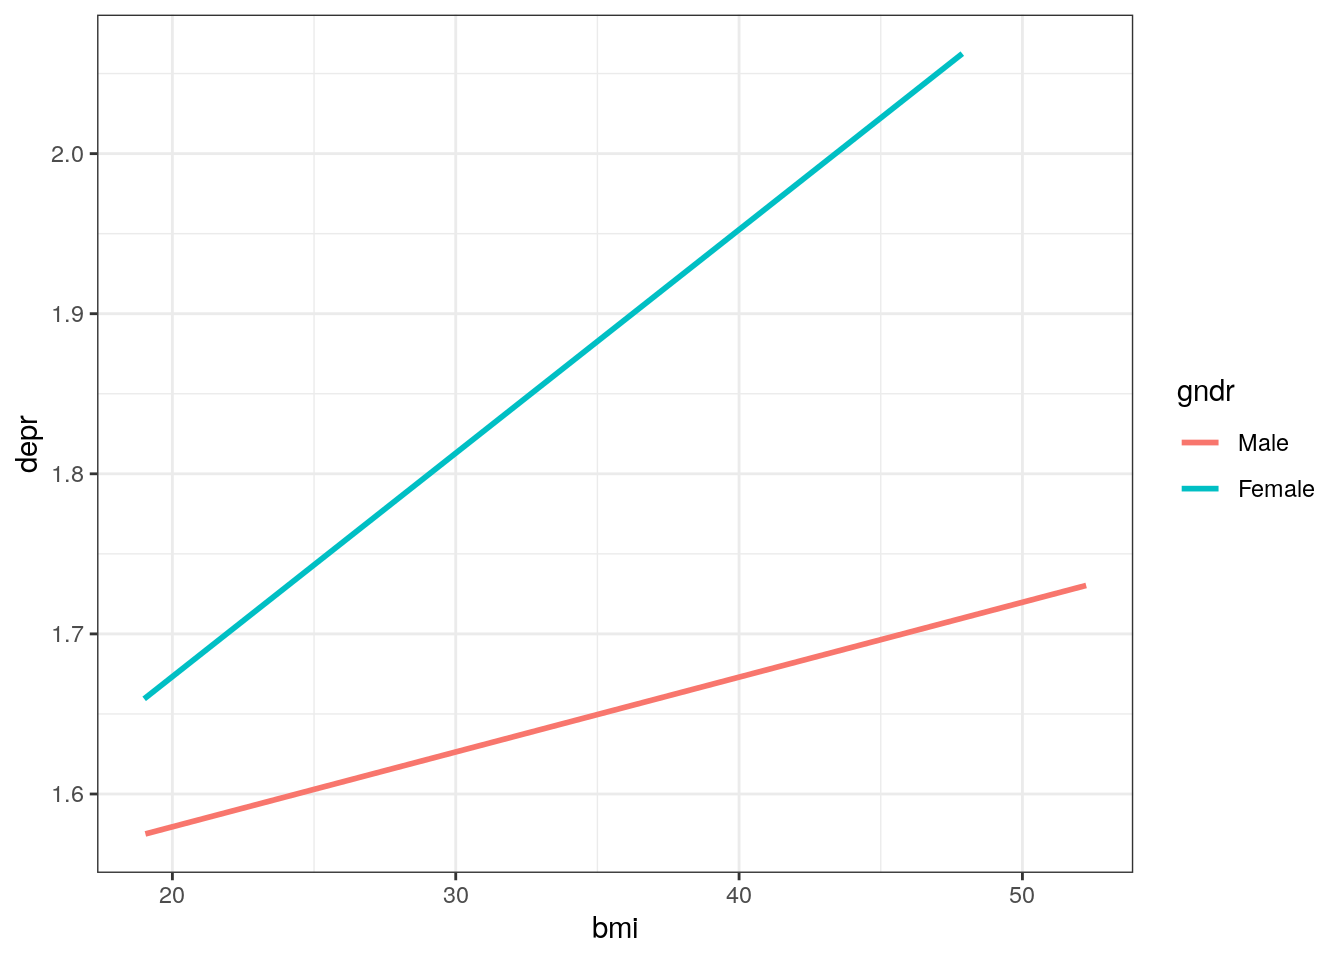
\includegraphics[width=1\linewidth]{07-interaction-terms-in-linear-models_files/figure-latex/unnamed-chunk-9-1} 

}

\caption{ggplot automatically includes interaction}\label{fig:unnamed-chunk-9}
\end{figure}

\hypertarget{example-3-link-between-working-hours-income-and-life-satisfaction}{%
\section{Example 3: link between working hours, income and life satisfaction}\label{example-3-link-between-working-hours-income-and-life-satisfaction}}

This example considers whether working hours (\texttt{wkhtot}) affect the link between income (\texttt{hinctnta}) and life satisfaction - i.e.~does working very long hours make income less valuable? This time, the effect appeared in the UK data in the 2014 European Social Survey - again, the question might be whether that is just an incident of spurious data mining, or whether it reveals a broader relationship.

In any case, let's have a look at the interaction. Note that \texttt{*} in the \texttt{lm()} formula is an abbreviation for \texttt{+} and \texttt{:}, so that the command below could also be written as \texttt{lm(stflife\ \textasciitilde{}\ wkhtot\ +\ hinctnta\ +\ wkhtot:hinctnta)}

\begin{Shaded}
\begin{Highlighting}[]
\NormalTok{essUK <-}\StringTok{ }\KeywordTok{filter}\NormalTok{(ess, cntry }\OperatorTok{==}\StringTok{ "GB"}\NormalTok{)}
\NormalTok{mod <-}\StringTok{ }\KeywordTok{lm}\NormalTok{(stflife }\OperatorTok{~}\StringTok{ }\NormalTok{wkhtot}\OperatorTok{*}\NormalTok{hinctnta, essUK) }
\KeywordTok{summary}\NormalTok{(mod)}
\end{Highlighting}
\end{Shaded}

\begin{verbatim}
## 
## Call:
## lm(formula = stflife ~ wkhtot * hinctnta, data = essUK)
## 
## Residuals:
##     Min      1Q  Median      3Q     Max 
## -7.9013 -0.9305  0.3023  1.3331  3.6527 
## 
## Coefficients:
##                  Estimate Std. Error t value Pr(>|t|)    
## (Intercept)      6.085338   0.242722  25.071  < 2e-16 ***
## wkhtot           0.008065   0.006235   1.293   0.1960    
## hinctnta         0.238197   0.043684   5.453 5.64e-08 ***
## wkhtot:hinctnta -0.002129   0.001055  -2.019   0.0437 *  
## ---
## Signif. codes:  0 '***' 0.001 '**' 0.01 '*' 0.05 '.' 0.1 ' ' 1
## 
## Residual standard error: 2.023 on 1810 degrees of freedom
##   (450 observations deleted due to missingness)
## Multiple R-squared:  0.05154,	Adjusted R-squared:  0.04997 
## F-statistic: 32.79 on 3 and 1810 DF,  p-value: < 2.2e-16
\end{verbatim}

We can see that while income positively predicts life satisfaction, this effects appears to be weaker when both income and working hours are high. However, we need to be careful with interpretation here - technically, the coefficients for income and working hours now reflect the impact of that variable when the other variable is 0, and are thus unlikely to be meaningful. Therefore, it is better to look at the interaction plot and at simple slopes analyses. Both can now be done in two ways, depending on which variable we see as the primary predictor/variable of interest.

\begin{Shaded}
\begin{Highlighting}[]
\KeywordTok{interact_plot}\NormalTok{(mod, }\DataTypeTok{pred=}\StringTok{"hinctnta"}\NormalTok{, }\DataTypeTok{modx =} \StringTok{"wkhtot"}\NormalTok{)}
\end{Highlighting}
\end{Shaded}

\begin{figure}

{\centering 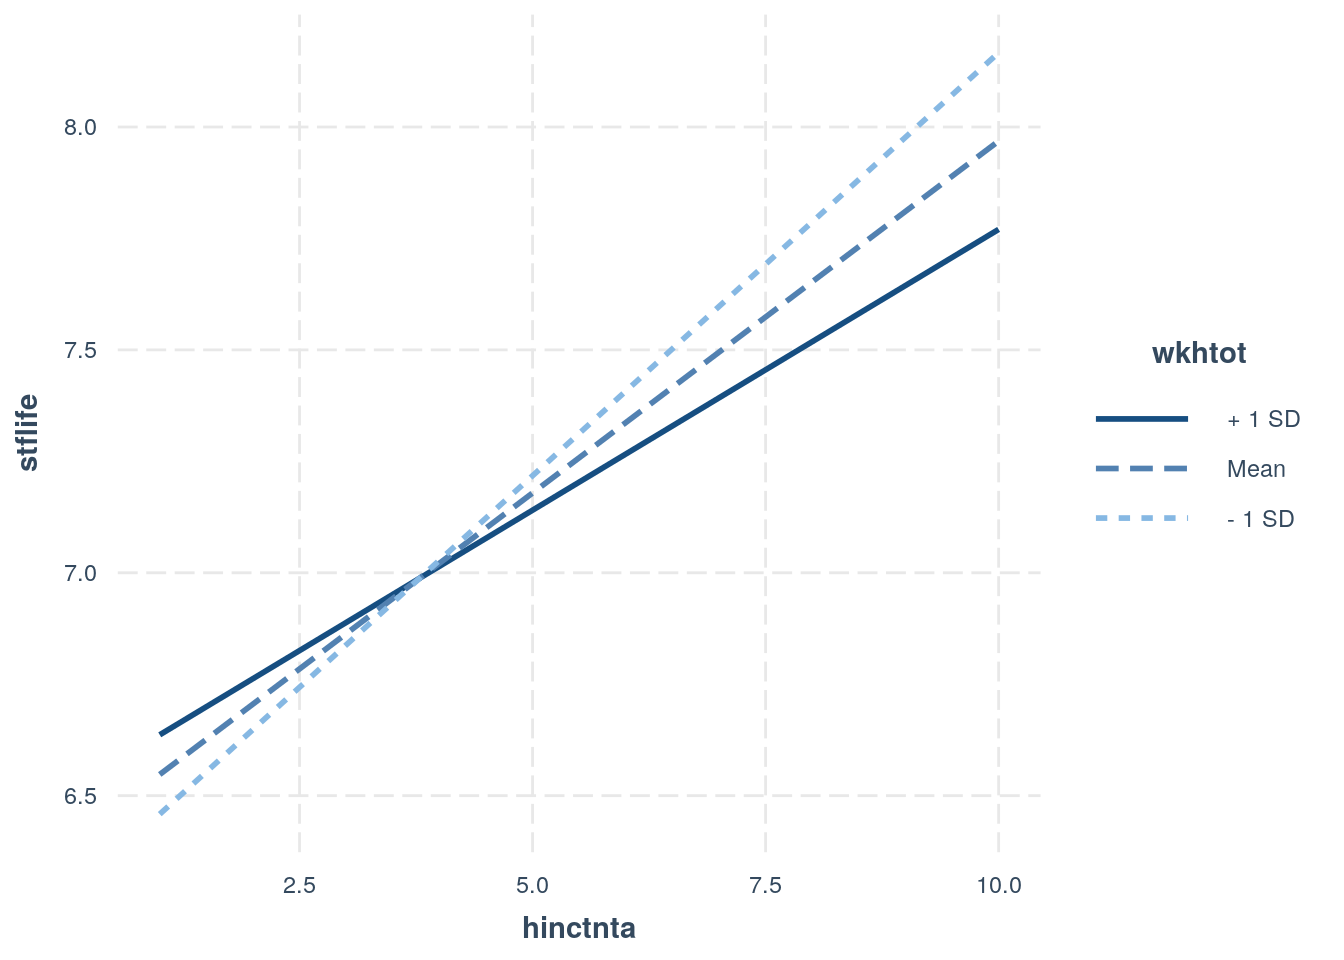
\includegraphics[width=1\linewidth]{07-interaction-terms-in-linear-models_files/figure-latex/unnamed-chunk-11-1} 

}

\caption{Option A: strong positive effect of income, tempered by working hours}\label{fig:unnamed-chunk-11}
\end{figure}

\begin{Shaded}
\begin{Highlighting}[]
\KeywordTok{interact_plot}\NormalTok{(mod, }\DataTypeTok{pred=}\StringTok{"wkhtot"}\NormalTok{, }\DataTypeTok{modx =} \StringTok{"hinctnta"}\NormalTok{)}
\end{Highlighting}
\end{Shaded}

\begin{figure}

{\centering 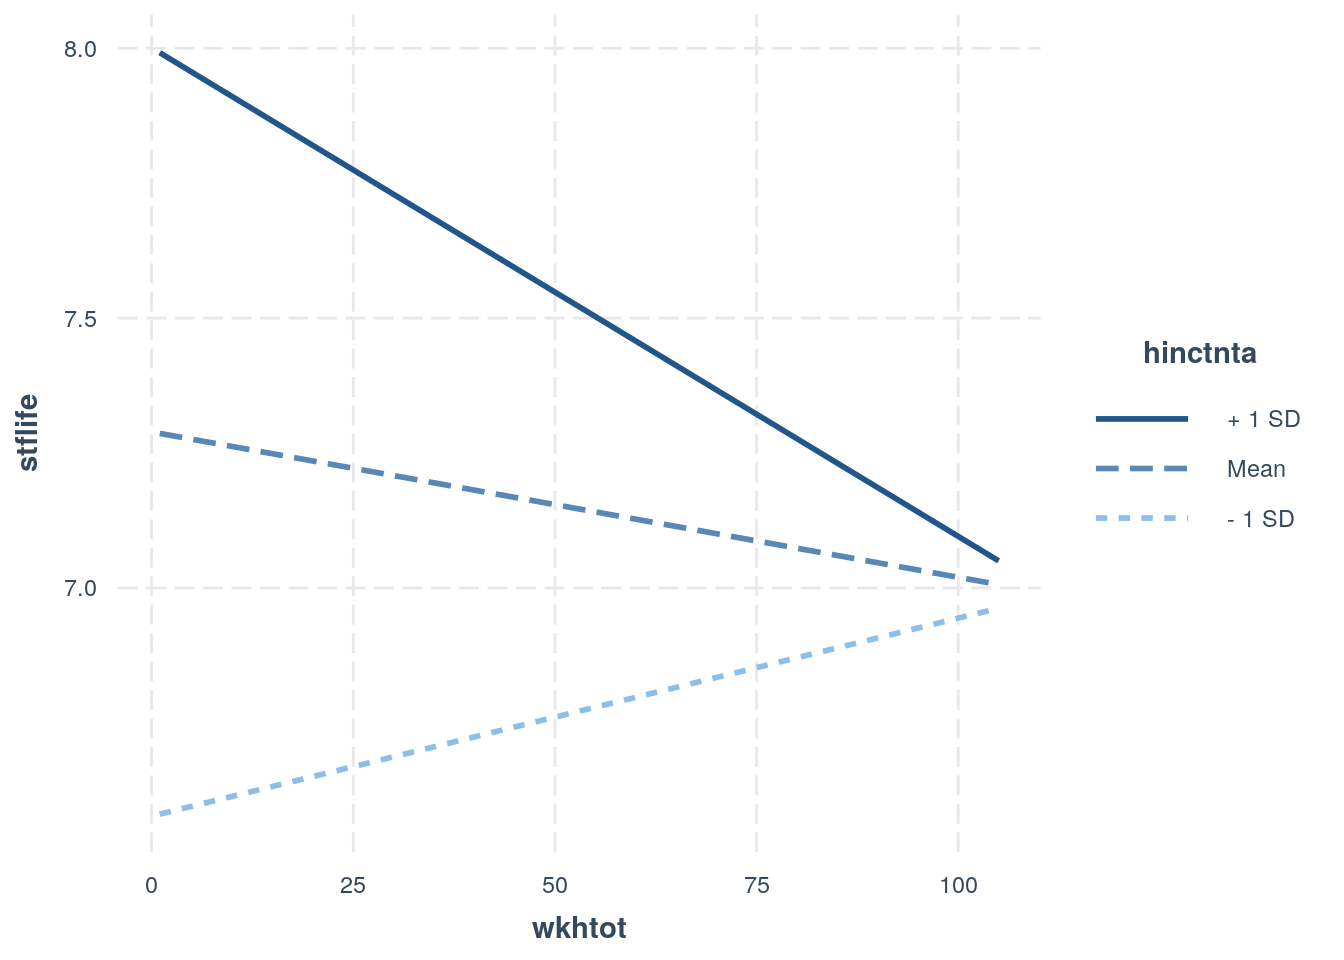
\includegraphics[width=1\linewidth]{07-interaction-terms-in-linear-models_files/figure-latex/unnamed-chunk-12-1} 

}

\caption{Option B: very different effects of working hours, depending on income}\label{fig:unnamed-chunk-12}
\end{figure}

Simple slopes analyses (\texttt{sim\_slopes()}) offer similar information together with significance tests and thus help to decide which of the slopes should be interpreted. They contain the Johnson-Neyman interval, which is the range of values of the moderator for which the predictor has a significant effect on the outcome.

\begin{Shaded}
\begin{Highlighting}[]
\NormalTok{pacman}\OperatorTok{::}\KeywordTok{p_load}\NormalTok{(interactions)}
\KeywordTok{sim_slopes}\NormalTok{(mod, }\DataTypeTok{pred=}\StringTok{"hinctnta"}\NormalTok{, }\DataTypeTok{modx =} \StringTok{"wkhtot"}\NormalTok{)}
\end{Highlighting}
\end{Shaded}

\begin{verbatim}
## JOHNSON-NEYMAN INTERVAL 
## 
## When wkhtot is OUTSIDE the interval [74.17, 2622.20], the slope of hinctnta
## is p < .05.
## 
## Note: The range of observed values of wkhtot is [1.00, 105.00]
## 
## SIMPLE SLOPES ANALYSIS 
## 
## Slope of hinctnta when wkhtot = 22.73 (- 1 SD): 
## 
##   Est.   S.E.   t val.      p
## ------ ------ -------- ------
##   0.19   0.02     8.19   0.00
## 
## Slope of hinctnta when wkhtot = 37.72 (Mean): 
## 
##   Est.   S.E.   t val.      p
## ------ ------ -------- ------
##   0.16   0.02     9.76   0.00
## 
## Slope of hinctnta when wkhtot = 52.71 (+ 1 SD): 
## 
##   Est.   S.E.   t val.      p
## ------ ------ -------- ------
##   0.13   0.02     5.71   0.00
\end{verbatim}

\begin{Shaded}
\begin{Highlighting}[]
\KeywordTok{sim_slopes}\NormalTok{(mod, }\DataTypeTok{pred=}\StringTok{"wkhtot"}\NormalTok{, }\DataTypeTok{modx =} \StringTok{"hinctnta"}\NormalTok{)}
\end{Highlighting}
\end{Shaded}

\begin{verbatim}
## JOHNSON-NEYMAN INTERVAL 
## 
## When hinctnta is OUTSIDE the interval [-43.03, 7.73], the slope of wkhtot
## is p < .05.
## 
## Note: The range of observed values of hinctnta is [1.00, 10.00]
## 
## SIMPLE SLOPES ANALYSIS 
## 
## Slope of wkhtot when hinctnta = 2.07 (- 1 SD): 
## 
##   Est.   S.E.   t val.      p
## ------ ------ -------- ------
##   0.00   0.00     0.81   0.42
## 
## Slope of wkhtot when hinctnta = 5.05 (Mean): 
## 
##    Est.   S.E.   t val.      p
## ------- ------ -------- ------
##   -0.00   0.00    -0.84   0.40
## 
## Slope of wkhtot when hinctnta = 8.04 (+ 1 SD): 
## 
##    Est.   S.E.   t val.      p
## ------- ------ -------- ------
##   -0.01   0.00    -2.01   0.04
\end{verbatim}

Finally, the \texttt{johnson\_neyman()} function creates a plot showing the slope of one variable depending on the value of the other, while highlighting the regions of significance. This can help with an understanding of the relationship, but is not (yet?) widely used.

\begin{Shaded}
\begin{Highlighting}[]
\KeywordTok{johnson_neyman}\NormalTok{(mod, }\DataTypeTok{pred=}\StringTok{"wkhtot"}\NormalTok{, }\DataTypeTok{modx =} \StringTok{"hinctnta"}\NormalTok{)}
\end{Highlighting}
\end{Shaded}

\begin{verbatim}
## JOHNSON-NEYMAN INTERVAL 
## 
## When hinctnta is OUTSIDE the interval [-43.03, 7.73], the slope of wkhtot
## is p < .05.
## 
## Note: The range of observed values of hinctnta is [1.00, 10.00]
\end{verbatim}

\begin{figure}

{\centering 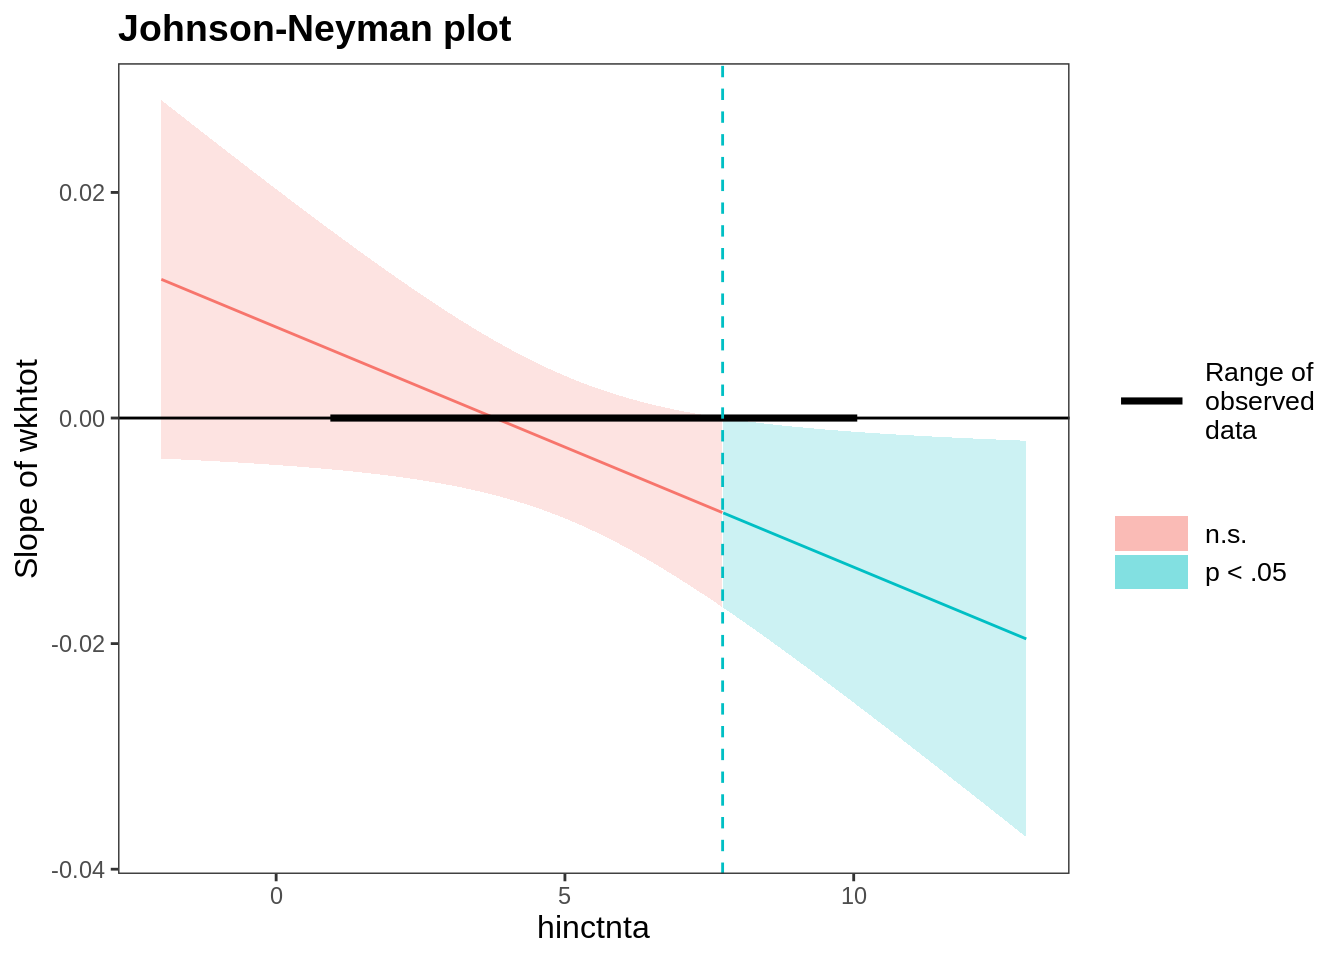
\includegraphics[width=1\linewidth]{07-interaction-terms-in-linear-models_files/figure-latex/unnamed-chunk-14-1} 

}

\caption{Johnson-Neyman plot shows regions of significance}\label{fig:unnamed-chunk-14}
\end{figure}

\hypertarget{chi-squared-tests-for-associations-between-categorical-variables}{%
\chapter{Chi-squared tests for associations between categorical variables}\label{chi-squared-tests-for-associations-between-categorical-variables}}

Watch this video for an introduction to this topic:

When we want to see whether two categorical variables are associated with each other, typical linear models won't work. Instead, we need a new way to decide whether a difference between the data we observe and that which we expect under the null-hypothesis is unlikely to occur due to chance. But before we get to that, we should look at the data.

\hypertarget{tables-of-frequencies-and-proportions}{%
\section{Tables of frequencies and proportions}\label{tables-of-frequencies-and-proportions}}

With two categorical variables, the data we observe can best be shown in a frequency table - i.e.~a table that shows how many observations fall into each combination of categories of the two variables. This is created with the \texttt{table()} function. Let's look an example of the association between political parties and their winning candidates' gender in the 2019 UK general election. (Note that this is based on the official statistics published by the election authorities, who registered candidate gender as a binary variable.)

\begin{Shaded}
\begin{Highlighting}[]
\KeywordTok{table}\NormalTok{(constituencies}\OperatorTok{$}\NormalTok{ElectionWon, constituencies}\OperatorTok{$}\NormalTok{WinnerGender)}
\end{Highlighting}
\end{Shaded}

\begin{verbatim}
##      
##       Female Male
##   Con     87  278
##   Lab    104   98
##   LD       7    4
##   SNP     16   32
\end{verbatim}

If there is an association between the two variables, then the proportional distribution will differ between the rows (i.e.~one party would have a higher \emph{share} of women than another party). To see whether that is the case, proportion tables that show shares are helpful. These can be created from the \texttt{table()} output with the \texttt{prop.table()} function. However, there are three options for proportions: are we interested in the share of each cell as a part of the total number of candidates? Or as a share of all winning candidates of a gender (i.e what share of female winning candidates are from the Conservative party)? Or rather the shares of women and men as a share of the total winning candidates of each party? In this case the latter seems most relevant and interpretable.

\begin{Shaded}
\begin{Highlighting}[]
\NormalTok{x <-}\StringTok{ }\KeywordTok{table}\NormalTok{(constituencies}\OperatorTok{$}\NormalTok{ElectionWon, constituencies}\OperatorTok{$}\NormalTok{WinnerGender)}
\CommentTok{#prop.table(x) - share of each cell as part of the total}
\CommentTok{#prop.table(x, margin = 2) - share of each cell as part of the column}
\KeywordTok{prop.table}\NormalTok{(x, }\DataTypeTok{margin =} \DecValTok{1}\NormalTok{) }\OperatorTok\StringTok{ }\CommentTok{#Share of each cell as part of the row}
\StringTok{   }\KeywordTok{round}\NormalTok{(}\DecValTok{2}\NormalTok{) }\CommentTok{#Round to 2 decimal places}
\end{Highlighting}
\end{Shaded}

\begin{verbatim}
##      
##       Female Male
##   Con   0.24 0.76
##   Lab   0.51 0.49
##   LD    0.64 0.36
##   SNP   0.33 0.67
\end{verbatim}

\hypertarget{the-null-hypothesis-and-the-chi2-statistic}{%
\section{\texorpdfstring{The null hypothesis and the \(\chi^2\) statistic}{The null hypothesis and the \textbackslash chi\^{}2 statistic}}\label{the-null-hypothesis-and-the-chi2-statistic}}

To be able to test whether any differences between the rows or between the columns that we observe in a frequency table are statistically significant, we need to be clear on what the null hypothesis is. If two variables are statistically independent, then their distribution needs to be the same across each row and along each column. This does not mean that all cells need to have the same value, In our case, given that there are many more male than female election winners and many more Conservative MPs than MPs of any other party, we would expect the male Conservatives cell to have the highest number of observations if there was no relationship between party and winning candidates' gender, i.e.~if the null hypothesis was true.

The expected number of observations in each cell under the null hypothesis can be calculated as the share of its entire row of the total observations (e.g., the total share of female candidates) * the share of its entire column of the total (e.g., the total share of Labour candidates) * the total number of observations. Based on that logic, the expected number of observations per cell would be the following.

\begin{verbatim}
##                           constituencies$WinnerGender
## constituencies$ElectionWon Female Male
##                        Con    125  240
##                        Lab     69  133
##                        LD       4    7
##                        SNP     16   32
\end{verbatim}

Once we know what to expect under the null-hypothesis, we need a way to see how far our observed data diverges from that. The \(\chi^2\) (chi-squared) test statistic provides a way of measuring that distance in a way that is independent of our sample size and therefore comparable across studies. It is calculated as follows, where O is the \emph{observed} number of cases per cell of the frequency table and E is the \emph{expected} number under the null-hypothesis:

\[\chi^2=\sum\frac{(O-E)^2}E\]

In R, easiest way to calculate it and test whether the distance of the observed distribution from the null distribution is statistically significant is to use the \texttt{chisq.test()} function.

\hypertarget{the-chisq.test-function}{%
\section{The chisq.test() function}\label{the-chisq.test-function}}

As a simple fictional example, we might be interested in whether Scottish and British people differ in their preference for tea versus coffee. If we ask 100 people, we might observe the following distribution:

\begin{Shaded}
\begin{Highlighting}[]
\KeywordTok{table}\NormalTok{(prefData}\OperatorTok{$}\NormalTok{nationality, prefData}\OperatorTok{$}\NormalTok{preference)}
\end{Highlighting}
\end{Shaded}

\begin{verbatim}
##           
##            Coffee Tea
##   English      45  95
##   Scottish     30  30
\end{verbatim}

To calculate the distance from distribution expected if there was no association between nationality and tea preference, we use the chisq.test() function. That also gives us an associated \emph{p}-value.

\begin{Shaded}
\begin{Highlighting}[]
\KeywordTok{chisq.test}\NormalTok{(prefData}\OperatorTok{$}\NormalTok{nationality, prefData}\OperatorTok{$}\NormalTok{preference, }\DataTypeTok{correct =} \OtherTok{FALSE}\NormalTok{)}
\end{Highlighting}
\end{Shaded}

\begin{verbatim}
## 
## 	Pearson's Chi-squared test
## 
## data:  prefData$nationality and prefData$preference
## X-squared = 5.7143, df = 1, p-value = 0.01683
\end{verbatim}

In this case, we would conclude that there is a statistically significant difference, with English people preferring tea more frequently than Scottish people do, \(\chi^2\)(1) = 4.98, \emph{p} = .016.

\hypertarget{dealing-with-small-samples}{%
\subsection{Dealing with small samples}\label{dealing-with-small-samples}}

When testing the significance of \(\chi^2\)-values, the calculated values are compared to a continuous distribution. When you have a small sample, however, your possible \(\chi^2\)-values cannot be continous; rather, a single observation shifting from one cell to another would be associated with a substantial jump in the \(\chi^2\) statistic. This can make the normal \emph{p}-values far too low in such cases, and therefore lead to Type I errors (false positives).

It is often recommended that \(\chi^2\) should not be used with samples where the expected frequency in more than 20\% of the cells is less than 5. In a 2x2 table (i.e when each of the two variables has only two possible categories), the Yates correction can be used to reduce the \(\chi^2\)-value and therefore make the test more conservative (R does that by default in \texttt{chisq.test()}, but it can be turned off by setting \texttt{correct\ =\ FALSE}). However, this sometimes goes too far, so my recommendation is to simulate \emph{p}-values for any samples where you have cells with low expected frequencies (say less than 20 expected cases in the smallest cell). You can do that by setting \texttt{simulate.p.value\ =\ TRUE} in the function call. Note that like any simulation, this is based on random number generation, so that \texttt{set.seed()} should be used with a fixed number of your choice to ensure that the results can be reproduced.

If we were to rerun the example above with a smaller sample but more extreme differences, we can compare the three possible methods of calculating \(\chi^2\). To see how small the smallest expected value is, we can look at the \texttt{expected} element of the output of the chisq.test() function.

\begin{Shaded}
\begin{Highlighting}[]
\KeywordTok{table}\NormalTok{(prefDataSmall}\OperatorTok{$}\NormalTok{nationality, prefDataSmall}\OperatorTok{$}\NormalTok{preference)}
\end{Highlighting}
\end{Shaded}

\begin{verbatim}
##           
##            Coffee Tea
##   English      12  30
##   Scottish     10   8
\end{verbatim}

\begin{Shaded}
\begin{Highlighting}[]
\KeywordTok{chisq.test}\NormalTok{(prefDataSmall}\OperatorTok{$}\NormalTok{nationality, prefDataSmall}\OperatorTok{$}\NormalTok{preference, }\DataTypeTok{correct =} \OtherTok{FALSE}\NormalTok{)}
\end{Highlighting}
\end{Shaded}

\begin{verbatim}
## 
## 	Pearson's Chi-squared test
## 
## data:  prefDataSmall$nationality and prefDataSmall$preference
## X-squared = 3.9508, df = 1, p-value = 0.04685
\end{verbatim}

It looks like the difference is significant. However, we should consider how small the smallest expected cell count is, to decide whether we need to adjust our way of testing significance. For that, we can look at the \texttt{expected} element of the output of the chisq.test() function.

\begin{Shaded}
\begin{Highlighting}[]
\KeywordTok{chisq.test}\NormalTok{(prefDataSmall}\OperatorTok{$}\NormalTok{nationality, prefDataSmall}\OperatorTok{$}\NormalTok{preference, }\DataTypeTok{correct =}\NormalTok{ F)}\OperatorTok{$}\NormalTok{expected}
\end{Highlighting}
\end{Shaded}

\begin{verbatim}
##                          prefDataSmall$preference
## prefDataSmall$nationality Coffee  Tea
##                  English    15.4 26.6
##                  Scottish    6.6 11.4
\end{verbatim}

With fewer than 7 expected cases of Scottish coffee drinkers, the standard \(\chi^2\) significance test is not reliable. Therefore, we either need to use the correction or simulation. Given that the simulation is based on random numbers, we should use the \texttt{set.seed()} function to initialise the random number generator - that makes sure that the results are reproducible.

\begin{Shaded}
\begin{Highlighting}[]
\KeywordTok{set.seed}\NormalTok{(}\DecValTok{300688}\NormalTok{)}
\KeywordTok{chisq.test}\NormalTok{(prefDataSmall}\OperatorTok{$}\NormalTok{nationality, prefDataSmall}\OperatorTok{$}\NormalTok{preference, }\DataTypeTok{correct =} \OtherTok{TRUE}\NormalTok{)}
\KeywordTok{chisq.test}\NormalTok{(prefDataSmall}\OperatorTok{$}\NormalTok{nationality, prefDataSmall}\OperatorTok{$}\NormalTok{preference, }\DataTypeTok{simulate.p.value =} \OtherTok{TRUE}\NormalTok{)}
\end{Highlighting}
\end{Shaded}

\begin{verbatim}
## 
## 	Pearson's Chi-squared test with Yates' continuity correction
## 
## data:  prefDataSmall$nationality and prefDataSmall$preference
## X-squared = 2.8742, df = 1, p-value = 0.09001
## 
## 
## 	Pearson's Chi-squared test with simulated p-value (based on 2000
## 	replicates)
## 
## data:  prefDataSmall$nationality and prefDataSmall$preference
## X-squared = 3.9508, df = NA, p-value = 0.07496
\end{verbatim}

These other two methods agree that caution is needed. Usually, the simulated \emph{p}-value will be a bit lower and a bit more accurate than the result of the Yates' continuity correction, so I would report that the data shows a trend towards a greater preference for tea among English respondents that falls short of the conventional standard of statistical significance, with \(\chi^2\) = 3.95, \emph{p} = .075 (based on 2000 Monte Carlo simulations).

\hypertarget{post-hoc-tests}{%
\section{Post-hoc tests}\label{post-hoc-tests}}

\(\chi^2\)-tests can be used to test for an association between variables with many different levels, such as music preferences or political parties. In that case, a significant result only tells us that at least one of the cell counts is significantly different from the expectation under the null-hypothesis. To get more details, post-hoc tests would be needed. To go back to the example at the start, let's test whether the winning candidates' gender differed significantly between the major UK parties in the 2019 General Election. It certainly looks that way from the proportions table, and the \texttt{chisq.test()} agrees

\begin{Shaded}
\begin{Highlighting}[]
\KeywordTok{prop.table}\NormalTok{(x, }\DataTypeTok{margin =} \DecValTok{1}\NormalTok{) }\OperatorTok\StringTok{ }\CommentTok{#Share of each cell as part of the row}
\StringTok{   }\KeywordTok{round}\NormalTok{(}\DecValTok{2}\NormalTok{) }\CommentTok{#Round to 2 decimal places}
\end{Highlighting}
\end{Shaded}

\begin{verbatim}
##      
##       Female Male
##   Con   0.24 0.76
##   Lab   0.51 0.49
##   LD    0.64 0.36
##   SNP   0.33 0.67
\end{verbatim}

\begin{Shaded}
\begin{Highlighting}[]
\KeywordTok{chisq.test}\NormalTok{(constituencies}\OperatorTok{$}\NormalTok{ElectionWon, constituencies}\OperatorTok{$}\NormalTok{WinnerGender,}
           \DataTypeTok{simulate.p.value =} \OtherTok{TRUE}\NormalTok{)}
\end{Highlighting}
\end{Shaded}

\begin{verbatim}
## 
## 	Pearson's Chi-squared test with simulated p-value (based on 2000
## 	replicates)
## 
## data:  constituencies$ElectionWon and constituencies$WinnerGender
## X-squared = 48.504, df = NA, p-value = 0.0004998
\end{verbatim}

However, this does not allow us to answer questions about any specific parties. For that, we need post-hoc tests. The most common tests compare each cell to its expected value under the null-hypothesis, but other tests are possible. For instance, you might be more interested to compare parties to each other rather than to this expected (average) value. For that, you would need to filter your data and run multiple chisq.tests.

To compare each cell to the expected value, we can use the \texttt{chisq.posthoc.test} package. This package contains the \texttt{chisq.posthoc.test()} function that takes a table as the input and computes standardised residuals (i.e.~distances) and \emph{p}-values for each cell. To avoid an inflated error rate, it can correct for multiple comparisons; by default the Bonferroni correction is used.

\begin{Shaded}
\begin{Highlighting}[]
\NormalTok{pacman}\OperatorTok{::}\KeywordTok{p_load}\NormalTok{(chisq.posthoc.test)}
\KeywordTok{table}\NormalTok{(constituencies}\OperatorTok{$}\NormalTok{ElectionWon, constituencies}\OperatorTok{$}\NormalTok{WinnerGender) }\OperatorTok\StringTok{ }\KeywordTok{chisq.posthoc.test}\NormalTok{(}\DataTypeTok{simulate.p.value =} \OtherTok{TRUE}\NormalTok{, }\DataTypeTok{method =} \StringTok{"bonferroni"}\NormalTok{)}
\end{Highlighting}
\end{Shaded}

\begin{verbatim}
##   Dimension     Value     Female       Male
## 1       Con Residuals -6.4559388  6.4559388
## 2       Con  p values  0.0000000  0.0000000
## 3       Lab Residuals  6.2985557 -6.2985557
## 4       Lab  p values  0.0000000  0.0000000
## 5        LD Residuals  2.0776181 -2.0776181
## 6        LD  p values  0.3019560  0.3019560
## 7       SNP Residuals -0.1295052  0.1295052
## 8       SNP  p values  1.0000000  1.0000000
\end{verbatim}

In this table, the \emph{p}-values can tell us which party/gender combinations differ significantly from the expectation under the null-hypothesis, while the sign of the residuals indicates the direction of the effect. Thus we can see that the Conservatives had significantly fewer male winning candidates while Labour had significantly more.

\emph{A note on statistical power and the importance of thinking about corrections:} This approach to running post-hoc tests runs one test per cell. In this situation with 2 genders and 4 parties, we have 8 cells, so that the Bonferroni correction multiplies each \emph{p}-value by 8, which makes it relatively hard to detect effects. However, as should be clear from the table, in cases where one variable has only two levels, half of the tests are redundant. If we know that the Conservatives have significantly fewer female winners, it follows necessarily that they have significantly more male winners. \emph{p}-values in each row are identical, and the residuals are symmetric. Therefore, we should only count half of the tests, and multiply p-values by 4 rather than 8. The general point is that it is essential to check how many tests a post-hoc functions counts in adjusting \emph{p}-values by comparing the \emph{p}-values reported when the adjustment parameter is set to ``none'' to those reported with ``bonferroni'' correction. Then make sure that you understand where that number comes from and that it makes sense in your situation.

\hypertarget{effect-sizes}{%
\section{Effect sizes}\label{effect-sizes}}

As always, finding that the variables are related to a statistically significant degree is only the first step, and you also want to report the strength of the relationship. Clear proportion tables are essential here, and then there are two options to sum up the strength of relationships into a single number: \textbf{Cramer's V} as a standardised measure of the strength of an association between two categorical variables, and the \textbf{Odds Ratio} of being in one cell rather than another.

\textbf{Cramer's V} describes a full table, and is scaled from 0 (no relationship) to 1 (one variable is entirely predictable by the other). It is often recommended that one should be weary of values greater than .5, as that suggests that the two variables might be redundant. Many packages offer functions to calculate Cramer's V, including the \texttt{effectsize} package that allows us to calculate it based on the \(\chi^2\)-value, the sample size, and the number of levels of each variable.

\begin{Shaded}
\begin{Highlighting}[]
\NormalTok{pacman}\OperatorTok{::}\KeywordTok{p_load}\NormalTok{(effectsize)}
\KeywordTok{chisq_to_cramers_v}\NormalTok{(}\DataTypeTok{chisq =} \FloatTok{48.5}\NormalTok{, }\DataTypeTok{n =} \DecValTok{626}\NormalTok{, }\DataTypeTok{nrow=}\DecValTok{4}\NormalTok{, }\DataTypeTok{ncol=}\DecValTok{2}\NormalTok{)}
\end{Highlighting}
\end{Shaded}

\begin{verbatim}
## Cramer's V |       95% CI
## -------------------------
## 0.28       | [0.19, 0.35]
\end{verbatim}

While this is a helpful statistic to compare effect strengths across multiple tests, it does not have an intuitive interpretation. Here, Odds Ratios might help. They can only be calculated for 2x2 tables, for instance for the fictional example regarding tea and coffee preferences.

\begin{verbatim}
##           
##            Coffee Tea
##   English      45  95
##   Scottish     30  30
\end{verbatim}

Here an \textbf{Odds Ratio} would state how much more likely it is to get a tea afficionado if we ask an English rather than a Scottish person. Odds are the ratio of the frequency of specified outcomes over the frequency of other outcomes. For instance, the odds of it being Sunday on a random day are 1 to 6. In this case, the odds for getting a tea afficionado when picking out an English person would be 95:45, while they would be 30:30 for a Scottish person. Thus the odds ratio would be \[OR = \frac{\frac{95}{45}}{\frac{30}{30}}=2.1\] so that I would be

\begin{itemize}
\tightlist
\item
  2.1x more likely to get a tea afficionado rather than a coffee afficionado when picking out an English person from this sample than a Scottish person,
\item
  2.1x more likely to get a coffee afficionado rather than a tea afficionado when picking out a Scottish person rather than an English person from this sample,
\item
  2.1x more likely to have an English person in front of me when I encounter a tea afficionado from this sample,
\item
  and 2.1x more likely to have a Scottish person in front of me when I encounter a coffee afficionado from this sample.
\end{itemize}

All of these statements should be easier to interpret than a Cramer's V index of .17 (which happens to be the value of this sample). Of course you should pick which one of the ways of framing the relationship is the best answer to the question at hand, rather than reporting the same information multiple times.

\hypertarget{reporting-the-results-of-statistical-tests}{%
\chapter{Reporting the results of statistical tests}\label{reporting-the-results-of-statistical-tests}}

Statistical test can often result in a lot of different numbers, but should also result in clear decisions and messages. To facilitate communication, there are sets of guidelines regarding what to report. In this course, we are using the APA (American Psychological Association) guidelines, which are also commonly used in journals in psychology and beyond.

\hypertarget{essential-pieces-of-information}{%
\section{Essential pieces of information}\label{essential-pieces-of-information}}

When reporting inferential statistical tests, always make sure to:

\begin{itemize}
\tightlist
\item
  State whether the results were \textbf{significant} (or which results were), and what the exact \emph{p}-values were (typically rounded to three decimal places; if smaller than .001 then reported as \textless{} .001). Results with \emph{p}-values between .05 and .1 can be reported as a trend, or as marginally significant, but that should (usually) only be done if the estimated effect size is substantial.
\item
  Report \textbf{which test} you carried out, and how it was carried out, if you did anything non-standard (e.g., if \emph{p}-values were simulated). For each test, relevant degrees of freedom and test statistics should be reported, see below.
\item
  Include relevant \textbf{descriptive statistics}. If a difference is significant, the reader will want to know how large it was.
\item
  Consider including \textbf{effect sizes}, ideally with confidence intervals, so that readers can judge how important the effect is. In reality, there will often be some statistically significant differences between groups, but not all are of a size that makes them interesting or practically significant.
\end{itemize}

\hypertarget{what-to-include-for-specific-tests}{%
\subsection{What to include for specific tests}\label{what-to-include-for-specific-tests}}

\begin{itemize}
\tightlist
\item
  \textbf{\emph{t}-tests:} \emph{t}(df) = 1.23, \emph{p} = .012. df stands for degrees of freedom and is shown in the \texttt{t.test()}-output. If equal variances are assumed, it is the sample size - 1; otherwise, typically a bit less. In any case, it describes which \emph{t}-distribution was used to find the \emph{p}-value.
\item
  \textbf{\emph{F}-tests} (for ANOVAs and model evaluation): \emph{F}(df1, df2) = 1.23, \emph{p} = .012. Here you have two degrees of freedom, df1 for the model and df2 for the error term. Both are provided in the output of various functions; a simple heuristic for checking whether you got them the right way round is that df2 should be the larger one in the vast majority of cases.
\item
  \textbf{Correlations:} \emph{r} = .12, \emph{p} = .012. Given that correlations are bounded by -1 and 1, the leading 0 is always ommitted. If you use Spearman's rank order correlation, it is reported as \emph{rho} = .12; the Greek letter \(\rho\) is not typically used.
\item
  \textbf{\(\chi^2\)-tests:} \(\chi^2\)(df) = 1.23, \emph{p} = .012. Here the degrees of freedom are the number of frequency table rows - 1 * the number of columns - 1. When you \texttt{simulate.p.values}, R does not report it because it does not use a fixed \(\chi^2\)-distribution to look up the \emph{p}-values; you should report it nonetheless as it also gives an indication for the complexity of your hypothesis.
\end{itemize}

\textbf{Examples} can be found all over the internet; \href{http://ich.vscht.cz/~svozil/lectures/vscht/2015_2016/sad/APA_style2.pdf}{this} set of notes contains detailed instructions for most statistical tests.

\hypertarget{formatting}{%
\subsection{Formatting}\label{formatting}}

\begin{itemize}
\tightlist
\item
  Any \textbf{Roman letters} (\emph{p, r, F, t, R\^{}2, M}) that stand for specific statistics are printed in \emph{italics}
\item
  If a statistic cannot have a value higher than 1 (i.e.~for \emph{p, r, rho, R\^{}2}) the \textbf{leading 0} should be omitted, i.e.~\emph{p} = .04 rather than \emph{p} = 0.04
\item
  If you want to use \textbf{Greek letters} (e.g., \(\alpha, \beta, \chi, \Delta\)) in RMarkdown, the easiest way to get them is to create an inline formula (an expression wrapped into dollar signs) and then type the name of the letter after a \textbackslash, for instance \texttt{\$\textbackslash{}alpha\$} You can use the same approach to show sums, fractions etc., though you would generally not need that in this course. The easiest way to get special characters like Greek letters into Word documents is to Google and copy-paste them.
\item
  To insert a \textbf{superscript}, most often \^{}2, into RMarkdown, type \^{}2. In Word, there is a superscript button close to the font size selection box.
\item
  When it comes to \textbf{descriptive statistics}, \emph{N} typically denotes the number of cases/participants, \emph{M} the mean, and \emph{SD} the standard deviation
\end{itemize}

\hypertarget{rounding}{%
\subsection{Rounding}\label{rounding}}

It is important to round numbers consistently, partly because too many decimal places might convey a false impression of accuracy, but also because numbers that do not convey relevant information can quickly clutter up papers and presentations - or does it help if I report that I spend 2.978536776 hours working on this book today?

In general, test statistics and most descriptive statistics should be rounded to two decimal places (i.e.~places after the decimal point) and \emph{p}-values to three decimal places. If that leads to descriptive statistics or regression coefficients to be rounded down to 0.00, that is a strong indication that you should consider changing the scale of the variables (e.g., from hours to minutes). \emph{p}-values by definition can never be equal to 0, so here you need to pay attention to report small \emph{p}-values as \textless~.001 rather than =~.000

\textbf{How to round? (With one change to what you learned in school)} Cross out all numbers after the last decimal place you want to keep. If the first number you crossed out is less than 5, then you are done. If it more than 5, then increase the last number you keep by 1. If it is 5 and any later number if more than 0, then also increase the last number you keep by one. If it is exactly 5 with only 0s following, then keep the last number unchanged if it is even, and increase it by 1 if it is odd. Some examples:

\begin{itemize}
\tightlist
\item
  1.2349 --\textgreater{} 1.23
\item
  1.2351 --\textgreater{} 1.24
\item
  1.2350 --\textgreater{} 1.24
\item
  1.2250 --\textgreater{} 1.22 (!)
\end{itemize}

\emph{Why not just round up 5} like we all learned in school? If we always did that, we would introduce a small but consistent bias into our numbers. Therefore, this would better be randomised. The rule set out here goes towards randomisation without being too complicated, and is therefore what the APA guidelines recommend.

\hypertarget{survey-research---testing-scales}{%
\chapter{Survey research - testing scales}\label{survey-research---testing-scales}}

A lot of social science research is done with surveys. In this video, I am talking about some examples and challenges, as well as some ways of asking good questions. I am also talking about how to create scales that use multiple items to measure one construct, and how to test their internal consistency.

\hypertarget{creating-scales}{%
\section{Creating scales}\label{creating-scales}}

Often, surveys use multiple items to measure the same construct. This is particularly common when participants might be either unable or unwilling to answer a direct question (e.g., how racist are you?). In such cases, asking several related questions can help to get an overall measure of the construct, while reducing measurement error, because the errors on different items will cancel each other out (to some extent).

Once you have data on your items, the most common way of creating a scale is just to calculate the mean of the items. If some of them were worded in the opposite direction (known as reverse-coding, and often recommended to increase data quality), those items need to be reversed first, most easily by subtracting their value from 1 + the scale maximum. \footnote{The \texttt{alpha()} function from the \texttt{psych} package can support reverse-coding - or even automate it. To learn more, look at \texttt{?psych::alpha}}

\hypertarget{testing-internal-consistency}{%
\subsection{Testing internal consistency}\label{testing-internal-consistency}}

We might expect that our items all measure the same construct (e.g., prejudice against foreigners). However, we should test whether that is the case. The most common measure to use is \textbf{Cronbach's \(\alpha\)}. It ranges from 0 to 1, and can be roughly understood as the intercorrelation of all items. Here is how to calculate it in R, using some data from the European Social Survey 2014.

\begin{Shaded}
\begin{Highlighting}[]
\NormalTok{pacman}\OperatorTok{::}\KeywordTok{p_load}\NormalTok{(psych, tidyverse)}
\NormalTok{ess <-}\StringTok{ }\KeywordTok{read_rds}\NormalTok{(}\KeywordTok{url}\NormalTok{(}\StringTok{"http://empower-training.de/Gold/round7b.RDS"}\NormalTok{))}
\NormalTok{ess }\OperatorTok\StringTok{ }\KeywordTok{select}\NormalTok{(imtcjob, imbleco, imwbcrm) }\OperatorTok\StringTok{ }\NormalTok{psych}\OperatorTok{::}\KeywordTok{alpha}\NormalTok{()}
\end{Highlighting}
\end{Shaded}

\begin{verbatim}
## Number of categories should be increased  in order to count frequencies.
\end{verbatim}

\begin{verbatim}
## 
## Reliability analysis   
## Call: psych::alpha(x = .)
## 
##   raw_alpha std.alpha G6(smc) average_r S/N    ase mean  sd median_r
##       0.71      0.71    0.63      0.45 2.4 0.0025  4.4 1.8     0.45
## 
##  lower alpha upper     95% confidence boundaries
## 0.7 0.71 0.71 
## 
##  Reliability if an item is dropped:
##         raw_alpha std.alpha G6(smc) average_r S/N alpha se var.r med.r
## imtcjob      0.62      0.62    0.45      0.45 1.6   0.0038    NA  0.45
## imbleco      0.53      0.53    0.36      0.36 1.1   0.0047    NA  0.36
## imwbcrm      0.69      0.69    0.53      0.53 2.2   0.0031    NA  0.53
## 
##  Item statistics 
##             n raw.r std.r r.cor r.drop mean  sd
## imtcjob 38737  0.82  0.79  0.63   0.53  4.8 2.3
## imbleco 37872  0.83  0.83  0.71   0.60  4.5 2.2
## imwbcrm 38025  0.75  0.76  0.55   0.46  3.7 2.0
\end{verbatim}

The key part of the output is the standardised alpha value (\emph{std.alpha}). This indicates how internally consistent the scale is, and is usually interpreted in line with established cut-offs \citep{devellis2016scale}:

\begin{itemize}
\tightlist
\item
  \(\alpha\) \textless{} .6: poor,\\
\item
  0.6 ≤ \(\alpha\) ≤ .7: questionable,
\item
  0.7 ≤ \(\alpha\) ≤ .8: acceptable,
\item
  0.8 ≤ \(\alpha\) ≤ .9: good,
\item
  0.9 ≤ \(\alpha\): excellent.
\end{itemize}

However, it should be noted that \(\alpha\) increases with the length of the scale, so that a a short scale (e.g., 3 items) might well be of sufficient quality with \(\alpha\) = .65, while `excellent' levels of fit might require long scales that are costly or tiresome to administer.

The section on \emph{Reliability if an item is dropped} can be helpful when you find low internal consistency; in those cases it might be necessary to exclude items from the scale that reduce its consistency. Decisions about droppping items should not be made just on these numbers as that would risk overfitting your scale to the particular sample at hand. Instead, always also consider the content of the items.

\hypertarget{calculating-scale-scores}{%
\subsection{Calculating scale scores}\label{calculating-scale-scores}}

The \texttt{alpha()} function from the \texttt{psych} package automatically calculates scores for each participant on the scale. To use them, you need to save the object that the function returns and then access the \texttt{scores} element.

\begin{Shaded}
\begin{Highlighting}[]
\NormalTok{scale_data <-}\StringTok{ }\NormalTok{ess }\OperatorTok\StringTok{ }\KeywordTok{select}\NormalTok{(imtcjob, imbleco, imwbcrm) }\OperatorTok\StringTok{ }\NormalTok{psych}\OperatorTok{::}\KeywordTok{alpha}\NormalTok{()}
\CommentTok{#To print the details as above, just type scale_data}

\NormalTok{ess}\OperatorTok{$}\NormalTok{immigrant_attitudes <-}\StringTok{ }\NormalTok{scale_data}\OperatorTok{$}\NormalTok{scores}
\end{Highlighting}
\end{Shaded}

This calculates the mean of the items, automatically ignoring any missing values. If you prefer that participants who omitted one of the scale items have a missing value for the scale, it will be easiest to calculate the mean manually:

\begin{Shaded}
\begin{Highlighting}[]
\NormalTok{ess <-}\StringTok{ }\NormalTok{ess }\OperatorTok\StringTok{ }\KeywordTok{mutate}\NormalTok{(}\DataTypeTok{immigrant_attitudes =}\NormalTok{ (imbleco }\OperatorTok{+}\StringTok{ }\NormalTok{imtcjob }\OperatorTok{+}\StringTok{ }\NormalTok{imwbcrm)}\OperatorTok{/}\DecValTok{3}\NormalTok{)}
\end{Highlighting}
\end{Shaded}

\hypertarget{further-resources}{%
\section{Further resources}\label{further-resources}}

\begin{itemize}
\tightlist
\item
  You can check \href{https://socialresearchmethods.net/kb/types-of-reliability/\#internal-consistency-reliability}{this chapter} of the Research Methods Knowledge Base for more details on various measures of internal consistency (and of other forms of reliability)
\end{itemize}

\hypertarget{part-supplementary-topics}{%
\part*{Supplementary topics}\label{part-supplementary-topics}}
\addcontentsline{toc}{part}{Supplementary topics}

\hypertarget{accessing-online-data-sources}{%
\chapter{Accessing online data sources}\label{accessing-online-data-sources}}

This section introduces some examples of R packages that allow you to access large secondary datasets. They are often a good way to understand wider trends, and thereby provide a high-level justification for doing research into a specific question. However, they can also be data sources for research projects in their own right.

\hypertarget{world-bank-data}{%
\section{World Bank data}\label{world-bank-data}}

The World Bank offers a rich dataset with a particular focus on indicators relevant for the study of poverty, inequality and global development (in fact, much of gapminder is based on World Bank data). You can explore their data online on \href{https://data.worldbank.com}{data.worldbank.com}, or access it directly from R using the \texttt{wbstats} package.

Here, I will explore the question whether life expectancy and literacy have increased in line with GDP in the BRICS countries (Brasil, Russia, India, China and South Africa, a group that has often been seen as representing emerging economies).

\begin{Shaded}
\begin{Highlighting}[]
\NormalTok{pacman}\OperatorTok{::}\KeywordTok{p_load}\NormalTok{(tidyverse)}
\NormalTok{pacman}\OperatorTok{::}\KeywordTok{p_load}\NormalTok{(wbstats)}
\end{Highlighting}
\end{Shaded}

\begin{Shaded}
\begin{Highlighting}[]
\CommentTok{#Download current list of indicators}
\NormalTok{new_wb_cache <-}\StringTok{ }\KeywordTok{wb_cache}\NormalTok{()}

\CommentTok{#Search for indicators - you can best do this on data.worldbank.com }
\CommentTok{#and find the IndicatorID in the URL. The wbsearch() function also works}
\CommentTok{#but often returns too many hits.}

\CommentTok{#GDP per capita, purchasing power adjusted }
\CommentTok{#(to remove effect of exchange rates)}
\KeywordTok{wb_search}\NormalTok{(}\StringTok{"gdp.*capita.*PPP"}\NormalTok{, }\DataTypeTok{cache =}\NormalTok{ new_wb_cache)}
\end{Highlighting}
\end{Shaded}

\begin{verbatim}
## # A tibble: 4 x 3
##   indicator_id    indicator                indicator_desc                       
##   <chr>           <chr>                    <chr>                                
## 1 6.0.GDPpc_cons~ GDP per capita, PPP (co~ GDP per capita based on purchasing p~
## 2 NY.GDP.PCAP.PP~ GDP per capita, PPP (cu~ This indicator provides per capita v~
## 3 NY.GDP.PCAP.PP~ GDP per capita, PPP (co~ GDP per capita based on purchasing p~
## 4 NY.GDP.PCAP.PP~ GDP per capita, PPP ann~ Annual percentage growth rate of GDP~
\end{verbatim}

Once we know the names of the indicators, we can download them.

\begin{Shaded}
\begin{Highlighting}[]
\CommentTok{#Note: to get the country names, you can download all countries once }
\CommentTok{#and then check the names}
\CommentTok{#wb_dat <- wb(indicator = c("NY.GDP.PCAP.PP.KD", "SI.POV.GINI"), country = "all")}
\CommentTok{#wb_dat %>% count(iso2c, country) %>% view()            }
                            
\NormalTok{wb_dat <-}\StringTok{ }\KeywordTok{wb_data}\NormalTok{(}\DataTypeTok{indicator =} \KeywordTok{c}\NormalTok{(}\StringTok{"NY.GDP.PCAP.PP.KD"}\NormalTok{, }\StringTok{"SP.DYN.LE00.IN"}\NormalTok{, }\StringTok{"SE.TER.ENRR"}\NormalTok{), }
             \DataTypeTok{country =} \KeywordTok{c}\NormalTok{(}\StringTok{"IN"}\NormalTok{, }\StringTok{"BR"}\NormalTok{, }\StringTok{"CN"}\NormalTok{, }\StringTok{"ZA"}\NormalTok{, }\StringTok{"RU"}\NormalTok{), }\DataTypeTok{return_wide =} \OtherTok{FALSE}\NormalTok{)}
\end{Highlighting}
\end{Shaded}

Now we have the data in a ``long'' format - with one combination of countries, indicators and years per row. That is a good layout for plotting, for other analyses you would need to reshape the data into a wide format where each indicator is in its own variable - look for the spread() function if you need that.

A simple way of comparing the data is plotting the indicators side-by-side. One interesting take-away is that Brazil massively improved life expectancy and expanded education, even though GDP growth was rather modest, while South Africa stagnated in comparison.

\begin{Shaded}
\begin{Highlighting}[]
\CommentTok{#Our GDP series only starts in 1990 - so it does not make sense }
\CommentTok{#to consider earlier life expectancy}
\NormalTok{wb_datF <-}\StringTok{ }\NormalTok{wb_dat }\OperatorTok\StringTok{ }\KeywordTok{filter}\NormalTok{(}\KeywordTok{as.numeric}\NormalTok{(date)}\OperatorTok{>=}\DecValTok{1990}\NormalTok{)}

\KeywordTok{ggplot}\NormalTok{(wb_datF, }\KeywordTok{aes}\NormalTok{(}\DataTypeTok{x=}\KeywordTok{as.numeric}\NormalTok{(date), }\DataTypeTok{y=}\NormalTok{value, }\DataTypeTok{col=}\NormalTok{country)) }\OperatorTok{+}\StringTok{ }
\StringTok{  }\KeywordTok{geom_point}\NormalTok{() }\OperatorTok{+}\StringTok{ }\KeywordTok{geom_line}\NormalTok{() }\OperatorTok{+}\StringTok{ }
\StringTok{  }\KeywordTok{facet_wrap}\NormalTok{(.}\OperatorTok{~}\NormalTok{indicator, }\DataTypeTok{scales =} \StringTok{"free"}\NormalTok{, }\DataTypeTok{labeller =} \KeywordTok{labeller}\NormalTok{(}\DataTypeTok{indicator =} \KeywordTok{label_wrap_gen}\NormalTok{(}\DecValTok{25}\NormalTok{))) }\OperatorTok{+}
\StringTok{  }\CommentTok{#scales = "free" means that each indicator has its own y-axis, }
\StringTok{  }\CommentTok{#the labeller() function is needed for line breaks in the facet titles}
\StringTok{  }\KeywordTok{labs}\NormalTok{(}\DataTypeTok{title =} \StringTok{"Uneven progress in BRICS countries"}\NormalTok{, }\DataTypeTok{subtitle =} \StringTok{"World Bank data"}\NormalTok{, }
       \DataTypeTok{x =} \StringTok{"Year"}\NormalTok{, }\DataTypeTok{y=}\StringTok{""}\NormalTok{, }\DataTypeTok{col =} \StringTok{"Country"}\NormalTok{)}
\end{Highlighting}
\end{Shaded}

\begin{figure}

{\centering \includegraphics[width=1\linewidth]{11-accessing-online-data_files/figure-latex/unnamed-chunk-4-1} 

}

\caption{Example plot from World Bank data}\label{fig:unnamed-chunk-4}
\end{figure}

You can find a similar but slightly more detailed example for how to use the package \href{https://cengel.github.io/gearup2016/worldbank.html}{here} and very clear instructions in the the full \href{https://github.com/nset-ornl/wbstats/blob/master/README.md}{README file of the package}.

\hypertarget{wikidata}{%
\section{Wikidata}\label{wikidata}}

Wikidata is where most data from Wikipedia and much else lives. So if there are Wikipedia articles on the topic you are interested in, you can likely find underlying data on Wikidata. For example, this might be used to quickly extract data on the gender of heads of government of many countries.

Wikidata is based on data items that are connected by multiple relationships. So there would be an item for \emph{Germany}, an item for \emph{Angela Merkel} and a relationship for \emph{is the head of government of.} Similarly, there is an item for \emph{country} and a relationship for \emph{is an instance of} that connects it to \emph{Germany.} SPARQL queries are used to get the data - this \href{https://towardsdatascience.com/a-brief-introduction-to-wikidata-bb4e66395eb1}{article} explains the logic quite well, but unless you want to spend a couple more weeks learning how to code, you can just take \href{https://www.wikidata.org/wiki/Wikidata:SPARQL_query_service/queries/examples}{examples from Wikidata} and adjust them as needed. For adjusting them, the online \href{https://query.wikidata.org/}{Wikidata Query Service} works well, as it allows you to run the query again and again, until you get the data you need.

I got curious about what share of the world's population lives in countries with a female head of government, and how that varies by region. For that, I used the following code. (\texttt{gt} is a package to make nice tables easily.) \textbf{Note that a key step is missing: I did not clean the data.} It contains some duplicates, for instance because countries that span two continents are included twice in the Wikidata output. Data cleaning is a crucial part of analysing online data, but not the focus of this chapter.

\begin{Shaded}
\begin{Highlighting}[]
\NormalTok{pacman}\OperatorTok{::}\KeywordTok{p_load}\NormalTok{(WikidataQueryServiceR, gt)}

\NormalTok{headsOfGov <-}\StringTok{ }\KeywordTok{query_wikidata}\NormalTok{(}\StringTok{'}
\StringTok{SELECT ?country ?head ?gender ?countryLabel ?headLabel ?genderLabel  ?continentLabel ?governmentLabel ?population}
\StringTok{WHERE}
\StringTok{\{}
\StringTok{    ?country wdt:P31 wd:Q6256 .}
\StringTok{    ?country wdt:P6 ?head .}
\StringTok{    ?head wdt:P21 ?gender .  }
\StringTok{    ?country wdt:P30 ?continent . }
\StringTok{    ?country wdt:P1082 ?population .}
\StringTok{    SERVICE wikibase:label \{ bd:serviceParam wikibase:language "en" \}}
\StringTok{\}}
\StringTok{ORDER BY ?countryLabel}
\StringTok{'}\NormalTok{)}

\NormalTok{regional <-}\StringTok{ }\NormalTok{headsOfGov }\OperatorTok\StringTok{ }\KeywordTok{group_by}\NormalTok{(continentLabel, genderLabel) }\OperatorTok\StringTok{ }\KeywordTok{summarise}\NormalTok{(}\DataTypeTok{pop =} \KeywordTok{sum}\NormalTok{(population), }\DataTypeTok{n =} \KeywordTok{n}\NormalTok{()) }\OperatorTok\StringTok{ }\KeywordTok{ungroup}\NormalTok{()}

\NormalTok{world <-}\StringTok{ }\KeywordTok{data.frame}\NormalTok{(}\DataTypeTok{continentLabel =} \StringTok{"World"}\NormalTok{, }
\NormalTok{               headsOfGov }\OperatorTok\StringTok{ }\KeywordTok{group_by}\NormalTok{(genderLabel) }\OperatorTok
\StringTok{                 }\KeywordTok{summarise}\NormalTok{(}\DataTypeTok{pop=}\KeywordTok{sum}\NormalTok{(population), }\DataTypeTok{n=}\KeywordTok{n}\NormalTok{()), }
               \DataTypeTok{stringsAsFactors =} \OtherTok{FALSE}\NormalTok{)}


\NormalTok{world }\OperatorTok\StringTok{ }\KeywordTok{mutate}\NormalTok{(}\DataTypeTok{ShareOfCountries =}\NormalTok{ n}\OperatorTok{/}\KeywordTok{sum}\NormalTok{(n)}\OperatorTok{*}\DecValTok{100}\NormalTok{, }\DataTypeTok{ShareOfPopulation =}\NormalTok{ pop}\OperatorTok{/}\KeywordTok{sum}\NormalTok{(pop)}\OperatorTok{*}\DecValTok{100}\NormalTok{) }\OperatorTok\StringTok{ }\KeywordTok{filter}\NormalTok{(genderLabel }\OperatorTok{==}\StringTok{ "female"}\NormalTok{) }\OperatorTok\StringTok{ }\KeywordTok{select}\NormalTok{(ShareOfCountries, ShareOfPopulation) }\OperatorTok\StringTok{ }\KeywordTok{round}\NormalTok{(}\DecValTok{1}\NormalTok{) }\OperatorTok\StringTok{ }\NormalTok{gt}\OperatorTok{::}\KeywordTok{gt}\NormalTok{() }\OperatorTok\StringTok{ }\NormalTok{gt}\OperatorTok{::}\KeywordTok{tab_header}\NormalTok{(}\DataTypeTok{title=}\NormalTok{gt}\OperatorTok{::}\KeywordTok{md}\NormalTok{(}\StringTok{"**Women rule**"}\NormalTok{), }\DataTypeTok{subtitle =} \StringTok{"*Percent*"}\NormalTok{)}

\NormalTok{regionalAndWorld <-}\StringTok{ }\KeywordTok{rbind}\NormalTok{(regional, world)}
\end{Highlighting}
\end{Shaded}

\captionsetup[table]{labelformat=empty,skip=1pt}
\begin{longtable}{rr}
\caption*{
\large \textbf{Women rule}\\ 
\small *Percent*\\ 
} \\ 
\toprule
ShareOfCountries & ShareOfPopulation \\ 
\midrule
8.8 & 4.5 \\ 
\bottomrule
\end{longtable}

\begin{Shaded}
\begin{Highlighting}[]
\KeywordTok{ggplot}\NormalTok{(regionalAndWorld, }\KeywordTok{aes}\NormalTok{(}\DataTypeTok{x=}\NormalTok{continentLabel, }\DataTypeTok{y=}\NormalTok{pop, }\DataTypeTok{fill=}\NormalTok{genderLabel)) }\OperatorTok{+}\StringTok{ }\KeywordTok{geom_col}\NormalTok{(}\DataTypeTok{position=}\StringTok{"fill"}\NormalTok{) }\OperatorTok{+}\StringTok{ }
\StringTok{    }\CommentTok{#Turns chart into bars rather than columns}
\StringTok{    }\KeywordTok{coord_flip}\NormalTok{() }\OperatorTok{+}
\StringTok{    }\CommentTok{#Show percentages rather than fractions on y-axis (now shown as x-axis)}
\StringTok{    }\KeywordTok{scale_y_continuous}\NormalTok{(}\DataTypeTok{labels=}\NormalTok{scales}\OperatorTok{::}\NormalTok{percent) }\OperatorTok{+}
\StringTok{    }\KeywordTok{labs}\NormalTok{(}\DataTypeTok{title=}\StringTok{"Only a small fraction of the world's population is ruled by women"}\NormalTok{, }\DataTypeTok{subtitle=}\StringTok{"Source: WikiData, February 2020"}\NormalTok{, }\DataTypeTok{x=}\StringTok{""}\NormalTok{, }\DataTypeTok{y=}\StringTok{"Share of population"}\NormalTok{, }\DataTypeTok{fill=}\StringTok{"Head of government"}\NormalTok{)}
\end{Highlighting}
\end{Shaded}

\begin{figure}

{\centering \includegraphics[width=1\linewidth]{11-accessing-online-data_files/figure-latex/unnamed-chunk-6-1} 

}

\caption{Example plot from Wikidata}\label{fig:unnamed-chunk-6}
\end{figure}

\hypertarget{other-data-sources}{%
\section{Other data sources}\label{other-data-sources}}

Beyond the examples here, there are many other datasets to access. You might want to check out some of the following:

\begin{itemize}
\tightlist
\item
  The extensive \href{https://github.com/erikgahner/PolData}{list of political datasets} compiled by Erik Gahner, with lots of current and historical data on anything from terrorism to government revenues and gender in politics. At the bottom, it also has a list of links to other lists of datasets.
\item
  Eurostat offers a lot of statistics on all countries in Europe. In R, it can be accesses with the \texttt{eurostat} package; there is a good \href{https://github.com/rstudio/cheatsheets/raw/master/eurostat.pdf}{cheatsheet} to help you get started
\item
  The webpage \href{http://asdfree.com/}{asdfree.com}, with (sparse) instructions of how to access a wide range of online data sources, from very focused surveys such as the US \emph{National Longitudinal Study of Adolescent to Adult Health} to international and very widely used datasets such as the \emph{World Values Survey.}
\item
  You can also use R to scrape data from pretty much any public webpage. \href{https://www.analyticsvidhya.com/blog/2017/03/beginners-guide-on-web-scraping-in-r-using-rvest-with-hands-on-knowledge/}{This tutorial} shows how to get data from IMDB, for instance.
\item
  Finally, the \texttt{essurvey} package is the easiest way to get data from the European Social Survey into R. There is a good example for how to use it \href{https://ropensci.org/blog/2018/06/14/essurvey/}{here}
\end{itemize}

\hypertarget{dealing-with-missing-data}{%
\chapter{Dealing with missing data}\label{dealing-with-missing-data}}

Missing data can pose serious problems for any data analysis.

\hypertarget{example}{%
\section{Example}\label{example}}

Let's imagine that we want to analyse the effect of a mentoring programme on boys and girls. For that, they take a test (score1), then experience the mentoring, and then take another test (score2). Let's load the required packages.

\begin{Shaded}
\begin{Highlighting}[]
\NormalTok{pacman}\OperatorTok{::}\KeywordTok{p_load}\NormalTok{(tidyverse) }\CommentTok{#As always}
\NormalTok{pacman}\OperatorTok{::}\KeywordTok{p_load}\NormalTok{(naniar) }\CommentTok{#To summarise and visualise missing data}
\NormalTok{pacman}\OperatorTok{::}\KeywordTok{p_load}\NormalTok{(simputation) }\CommentTok{#For imputation of missing data}
\end{Highlighting}
\end{Shaded}

I will simulate the data from our experiment as follows.

\begin{Shaded}
\begin{Highlighting}[]
\KeywordTok{set.seed}\NormalTok{(}\DecValTok{1234}\NormalTok{)}
\NormalTok{results <-}\StringTok{ }\KeywordTok{data.frame}\NormalTok{(}\DataTypeTok{gender =} \KeywordTok{c}\NormalTok{(}\KeywordTok{rep}\NormalTok{(}\StringTok{"M"}\NormalTok{, }\DecValTok{250}\NormalTok{), }\KeywordTok{rep}\NormalTok{(}\StringTok{"F"}\NormalTok{, }\DecValTok{250}\NormalTok{)), }
                      \DataTypeTok{score1 =} \KeywordTok{round}\NormalTok{(}\KeywordTok{c}\NormalTok{(}\KeywordTok{rnorm}\NormalTok{(}\DecValTok{250}\NormalTok{, }\DecValTok{45}\NormalTok{, }\DecValTok{10}\NormalTok{), }\KeywordTok{rnorm}\NormalTok{(}\DecValTok{250}\NormalTok{,}\DecValTok{60}\NormalTok{,}\DecValTok{10}\NormalTok{))), }
                      \DataTypeTok{score2 =} \KeywordTok{round}\NormalTok{(}\KeywordTok{c}\NormalTok{(}\KeywordTok{rnorm}\NormalTok{(}\DecValTok{250}\NormalTok{, }\DecValTok{55}\NormalTok{, }\DecValTok{10}\NormalTok{), }\KeywordTok{rnorm}\NormalTok{(}\DecValTok{250}\NormalTok{,}\DecValTok{70}\NormalTok{,}\DecValTok{10}\NormalTok{))))}

\NormalTok{results}\OperatorTok{$}\NormalTok{score2[results}\OperatorTok{$}\NormalTok{score1}\OperatorTok{<}\DecValTok{40}\NormalTok{] <-}\StringTok{ }\OtherTok{NA}
\end{Highlighting}
\end{Shaded}

Note that I have assumed that only students who pass the first test (i.e.~get at least 40) return to the second test. For all others, that data is missing. What pattern of missingness is that? MCAR MAR MNAR

Explanation

The data is \textbf{missing at random (MAR)} - whether score2 is missing depends on the value of score1, so that it is \emph{not} missing completely at random (MCAR). Whether score2 is missing does not depend on the value of score2 (beyond any association it might have with score1) - therefore it is also \emph{not} missing not at random (MNAR).

Let's see how much missing data that results in.

\begin{Shaded}
\begin{Highlighting}[]
\KeywordTok{miss_var_summary}\NormalTok{(results)}
\end{Highlighting}
\end{Shaded}

\begin{verbatim}
## # A tibble: 3 x 3
##   variable n_miss pct_miss
##   <chr>     <int>    <dbl>
## 1 score2       77     15.4
## 2 gender        0      0  
## 3 score1        0      0
\end{verbatim}

\hypertarget{case-deletion}{%
\subsection{Case deletion}\label{case-deletion}}

15\% missing data is quite a lot, but still within the range where analysts might choose to use case deletion and move on.

Given that the data is MAR, do you think that case deletion can bias the results? Yes No

Let's try case deletion, and test whether the effects on boys and girls are different.

\begin{Shaded}
\begin{Highlighting}[]
\NormalTok{resultsDel <-}\StringTok{ }\NormalTok{results }\OperatorTok\StringTok{ }\KeywordTok{na.omit}\NormalTok{() }\OperatorTok\StringTok{ }\CommentTok{#Deletes all rows with missing values}
\StringTok{                    }\KeywordTok{mutate}\NormalTok{(}\DataTypeTok{change =}\NormalTok{ score2 }\OperatorTok{-}\StringTok{ }\NormalTok{score1)}

\KeywordTok{t.test}\NormalTok{(change }\OperatorTok{~}\StringTok{ }\NormalTok{gender, resultsDel)}
\end{Highlighting}
\end{Shaded}

\begin{verbatim}
## 
## 	Welch Two Sample t-test
## 
## data:  change by gender
## t = 3.3375, df = 401.71, p-value = 0.000924
## alternative hypothesis: true difference in means is not equal to 0
## 95 percent confidence interval:
##  1.665645 6.440134
## sample estimates:
## mean in group F mean in group M 
##        9.008197        4.955307
\end{verbatim}

Here we would conclude with great confidence (\emph{p} \textless{} .001) that the intervention is more effective for girls than for boys. But given that we simulated the data ourselves, we know that the conclusion is false. It just arises because among the boys, the participants with the lowest scores who were most likely to score higher the next time round (\emph{regression to the mean}) did not show up for the second test. This shows that in such a case, imputation is critical.

\hypertarget{imputation}{%
\subsection{Imputation}\label{imputation}}

Imputation means filling in the gaps, to try to ensure that the dataset we use for our analysis looks as similar as possible to the complete dataset, without missing data.

For imputation, we need to decide how the missing data should be predicted based on the observed data. Here, it would seem to make most sense to use linear regression to predict score2 from score1. However, before we do that, we need to make sure that we can identify imputed values later on by saving which values were missing to begin with. We use two functions from the \texttt{naniar} package for that.

\begin{Shaded}
\begin{Highlighting}[]
\NormalTok{resultsImp <-}\StringTok{ }\NormalTok{results }\OperatorTok\StringTok{ }\KeywordTok{bind_shadow}\NormalTok{(}\DataTypeTok{only_miss =} \OtherTok{TRUE}\NormalTok{) }\OperatorTok\StringTok{ }\KeywordTok{add_label_missings}\NormalTok{()}

\KeywordTok{head}\NormalTok{(resultsImp)}
\end{Highlighting}
\end{Shaded}

\begin{verbatim}
## # A tibble: 6 x 5
##   gender score1 score2 score2_NA any_missing
##   <chr>   <dbl>  <dbl> <fct>     <chr>      
## 1 M          33     NA NA        Missing    
## 2 M          48     43 !NA       Not Missing
## 3 M          56     62 !NA       Not Missing
## 4 M          22     NA NA        Missing    
## 5 M          49     73 !NA       Not Missing
## 6 M          50     53 !NA       Not Missing
\end{verbatim}

\texttt{bind\_shadow()} has added a new column for each column that had missing values - in this case, \texttt{score2\_NA} was added, with two values showing whether the value was missing (NA) or not missing (!NA). Without the \texttt{only\_miss\ =\ \ TRUE} argument, it would add one `shadow' column for each column. \texttt{add\_label\_missings()} added just one new column (\texttt{any\_missing}) indicating whether there were any missing values in that row.

Now we can impute the missing data. Functions from the \texttt{simputation} package help with that.

\begin{Shaded}
\begin{Highlighting}[]
\NormalTok{resultsImp <-}\StringTok{ }\NormalTok{resultsImp }\OperatorTok\StringTok{ }\KeywordTok{group_by}\NormalTok{(gender) }\OperatorTok\StringTok{ }
\StringTok{  }\KeywordTok{impute_lm}\NormalTok{(score2 }\OperatorTok{~}\StringTok{ }\NormalTok{score1, }\DataTypeTok{add_residual =} \StringTok{"observed"}\NormalTok{) }
\end{Highlighting}
\end{Shaded}

This tells \texttt{simputation} to split the data by gender, calculate a regression to predict score2 from score1 for each gender, use that to impute score2 values and then \emph{add a residual} to each score2 value. The last part is crucial - if we don't do that, then all imputed values will be right on the regression line, which will artificially increase the correlation between score1 and score2 and the fit of any regression model we want to calculate later. \texttt{add\_residual} can either be \texttt{"observed"} or \texttt{"normal"}. In the first case, one of the observed residuals is randomly sampled, in the second case, the added residuals follow a normal distribution. I would always recommend \texttt{"observed"} as that makes one fewer assumption about the distribution of our data.

Let's see whether the imputed values look reasonable and whether they are different from the observed values in a way that they are likely to influence our results.

\begin{Shaded}
\begin{Highlighting}[]
\NormalTok{resultsImp <-}\StringTok{ }\NormalTok{resultsImp }\OperatorTok\StringTok{ }\KeywordTok{mutate}\NormalTok{(}\DataTypeTok{change =}\NormalTok{ score2 }\OperatorTok{-}\StringTok{ }\NormalTok{score1)}
\KeywordTok{ggplot}\NormalTok{(resultsImp, }\KeywordTok{aes}\NormalTok{(}\DataTypeTok{x=}\NormalTok{gender, }\DataTypeTok{y=}\NormalTok{change)) }\OperatorTok{+}\StringTok{ }\KeywordTok{geom_boxplot}\NormalTok{() }\OperatorTok{+}\StringTok{ }\KeywordTok{geom_jitter}\NormalTok{(}\KeywordTok{aes}\NormalTok{(}\DataTypeTok{color =}\NormalTok{ score2_NA))}
\end{Highlighting}
\end{Shaded}

\begin{figure}

{\centering 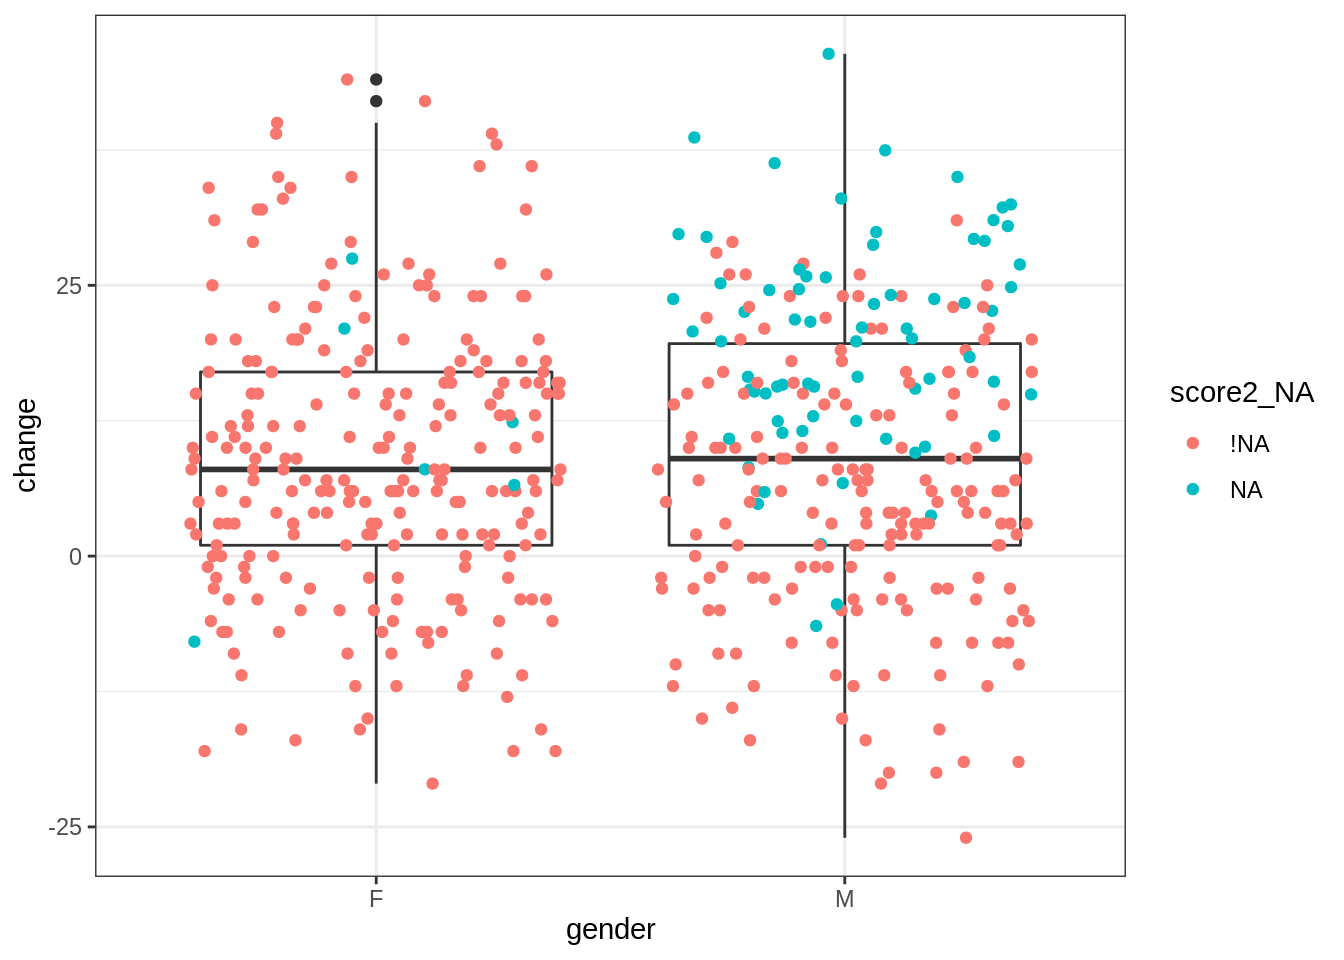
\includegraphics[width=1\linewidth]{12-dealing-with-missing-data_files/figure-latex/unnamed-chunk-7-1} 

}

\caption{Visualisation shows that imputed data matters}\label{fig:unnamed-chunk-7}
\end{figure}

Note that the colour aesthetic is only assigned inside \texttt{geom\_jitter()} (which is the same as geom\_point() but adds some random noise to the points to reduce overlap). If it was assigned within \texttt{ggplot()}, we would get separate boxplots for observed and imputed values, which is not the aim here.

Looking at the distribution of values that were missing and have now been imputed, we can see that the values are generally plausible, in that they fall within the observed range. However, particularly for boys, they are higher than the observed values and are therefore likely to influence our conclusion.

Let's test again whether there is a difference between boys and girls.

\begin{Shaded}
\begin{Highlighting}[]
\KeywordTok{t.test}\NormalTok{(change }\OperatorTok{~}\StringTok{ }\NormalTok{gender, resultsImp)}
\end{Highlighting}
\end{Shaded}

\begin{verbatim}
## 
## 	Welch Two Sample t-test
## 
## data:  change by gender
## t = -0.13676, df = 497.8, p-value = 0.8913
## alternative hypothesis: true difference in means is not equal to 0
## 95 percent confidence interval:
##  -2.459884  2.139711
## sample estimates:
## mean in group F mean in group M 
##        9.062020        9.222106
\end{verbatim}

This time, we get the correct result - there is no difference between boys and girls. This shows that when data is MAR (i.e.~when missingness depends on other variables we are interested in) we have to consider imputation.

\hypertarget{further-resources}{%
\section{Further resources}\label{further-resources}}

\begin{itemize}
\tightlist
\item
  The \href{https://cran.r-project.org/web/packages/naniar/vignettes/getting-started-w-naniar.html}{official vignette} for \texttt{naniar} provides provides good step-by-step instructions for exploring and visualising missing data
\item
  Similarly, the \href{https://cran.r-project.org/web/packages/simputation/vignettes/intro.html}{official vignette} for \texttt{simputation} contains details on how to use different imputation models and how to impute several variables at once
\end{itemize}

\hypertarget{probability-in-statistics-and-real-life}{%
\chapter{Probability in statistics and real life}\label{probability-in-statistics-and-real-life}}

Much of statistics (namely \emph{inferential} statistics) is about probability. Based on the data we have, is it likely that our hypothesis is true? But much of our other work as scientists, and much of everyday life, is also about probabilities. To be able to evaluate scientific claims, as well as news reporting and various situations in life, it helps to have a basic understanding of probability. By the end of this, you should be able to find an answer to questions like the following:

\begin{itemize}
\tightlist
\item
  How big does a group need to be until it is 95\% likely that two of them share a birthday?
\item
  Should it be news that there is a village in Poland where not a single boy has been born in more than a decade?
\item
  How likely is it that someone has breast cancer when they receive a positive mammogram result?
\end{itemize}

\hypertarget{what-are-probabilities}{%
\section{What are probabilities?}\label{what-are-probabilities}}

There is still a lot of technical disagreement on definitions in this area. However, for our purposes, we just need to distinguish three concepts: procedures, events and probabilities. \emph{Procedures} are anything that generates data - from rolling a die and writing down the number to conducting a medical test or surveying 500 people and calculating the mean on some outcome. An \emph{event} is the result of a procedure, be that a 3 on a die or a positive result on a medical test. Finally, the \emph{probability} expresses the likelihood with which an unobserved event will occur. Probabilities thereby offer guidance as to a reasonable degree of belief.

Probabilities can be based on experience and inference. I can count how often it rains later in the day when I wake up to a grey sky; if I do that for long enough and calculate the share of days when it rained as a total of all days I observed, this will give me a good guidance regarding the probability of rain. Weather forecasting apps do something a bit more sophisticated, but still quite similar.

Alternatively, we can use a more formal and logical way to find probabilities. This involves counting the number of possible outcomes of our procedure, and the number of possible outcomes that would lead to the event we are interested in. Probabilities are then expressed as fractions, dividing the number of ways in which our specified event can occur by the total number of outcomes. For example, the probability of rolling a 3 with a die is \(\frac{1}{6}\), as there are 6 possible outcomes, and only one of them results in a three. Rolling an even numbers, on the other hand, has a probability of \(\frac{3}{6}\) (or \(\frac{1}{2}\)) as there are now 3 out of 6 possible outcomes that lead to the event we are interested in.

Over to you - what is the probability of rolling a number smaller than 5? 2/6 or 1/3 3/6 or 1/2 4/6 or 2/3

These fractions can often be expressed more easily by a percentage. The probability of rolling an odd number is \(\frac{3}{6}\) or 50\%.

What is the probability of pulling a red card from a standard deck of cards, in percent?

Finally, probabilities can range from 0 (0 \%) to 1 (100 \%) - an event with a probability of 0 is impossible, one with a probability of 1 is inevitable.

\hypertarget{combining-multiple-events-together}{%
\section{Combining multiple events together}\label{combining-multiple-events-together}}

Often we are interested in more than one possible outcome, for instance when there are several paths to a desired outcome. So what is the probability of rolling an even number \emph{or} a 3 with a die? We already know that it is \(\frac{3}{6}\) for an even number and \(\frac{1}{6}\) for a 3. So the probability for either of them to occur is \(\frac{4}{6}\) - we can add them up.

However, what is the probability of rolling a 3 \emph{or} an odd number? The probability for rolling an odd number is \(\frac{3}{6}\), and the probability for rolling a 3 is \(\frac{1}{6}\). Can we add them up? Remember that probabilities are the ways in which the event we are interested in can occur, divided by the total number of outcomes. Here, those are three ways (1, 3 and 5) of the possible six outcomes of rolling a die. Since rolling a 3 satisfies both sides of our \emph{or} statement, we must not double count it.

As a shorthand, we can write \(P(A)\) to mean the probability of event A. Formally, the probability of either of two events occurring is
\(P(A or B)=P(A)+P(B)-P(AandB)\)

Over to you - what is the probability of getting a King or Queen when you draw a card from a standard deck of cards (52 cards)? 4/52 or 7.5 \% 8/52 or 15\% 16/52 or 30\%

I need a hint

Consider the total number of possible results as well as the possible number of ways you can get a King or a Queen

Give me the explanation

\(P(King)\) is \(\frac{4}{52}\) because there are 4 Kings among the 52 cards. Likewise, \(P(Queen)\) is \(\frac{4}{52}\) because there are 4 Queens. There is no card that is both a King and a Queen, so that we can just add up the probabilities and thus arrive at \(\frac{8}{52}\)

One more - what is the probability of getting a red card or a King or Queen when you draw a card from a standard deck of cards (52 cards)? 26/52 30/52 34/52

I need a hint

This time, there is a risk of double-counting. Avoid doing that.

Give me the explanation

\(P(KingorQueen)\) is \(\frac{8}{52}\), while \(P(Red)\) \(\frac{26}{52}\). However, there are 2 red Kings and 2 red Queens that are counted in both probabilities - therefore, we can get a red card or a King or a Queen in only 30 rather than 34 ways.

\hypertarget{looking-at-independent-events}{%
\section{Looking at independent events}\label{looking-at-independent-events}}

We are always interested in patterns that emerge when we look across multiple events. If we keep on tossing a coin, what is the probability to get two heads in a row? We can again count the number of possible outcomes versus the number of ways in which our event can occur.

\begin{figure}

{\centering 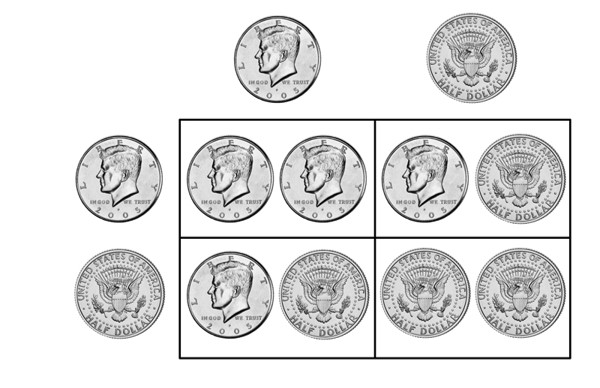
\includegraphics[width=1\linewidth]{./images/coins} 

}

\caption{Results of two coin tosses}\label{fig:img-coins}
\end{figure}

As you can see in the figure, there are four possible outcomes, only one of which results in two heads, so that the probability for that is \(\frac{1}{4}\) or 25\%. What about four coins in a row turning up head? We know that there is only one way in which that can happen, but how many outcomes are there in total? We have seen that 2 coins result in four outcomes. Now tossing a third coin results in two possibilities for each of these 4 outcomes so far, turning them into 8. Tossing a fourth coin results in 16. (If you can't see the pattern, try to draw out the possibilities - it will help.). So the probability for four heads in a row is \(\frac{1}{16}\) or about 6\%

The probability of two events both occurring in sequence is \(P(A)*P(B)\). That implies that the probability of the same event occurring n times in a row is \(P(A)^n\).

Over to you - if you assume that 50\% of babies born are girls, what is the probability of a woman to give birth to three girls in a row? 1/8 or 12.5\% 1/3 or 33 \% 1/2 or 50\%

Give me the explanation

The probability for the first child to be a girl is 50\% (\(\frac{1}{2}\)). For the second it is 50\% as well. If we multiply them, we get 25\%(\(\frac{1}{4}\)). The third child again has a 50\% chance of being a girl. Multiplying 25\% by 50\% results in 12.5\% (\(\frac{1}{8}\)).

Quite often we are interested in the \textbf{likelihood of something occurring at least once,} rather than on every attempt. So we might want to know how likely it is that a family with three children has at least one boy among them. Assuming that gender is binary, that is the same as saying that they do not have three girls. Given that they either have 3 girls or at least one boy, we know that these probabilities add up to 1 (certainty) - such events are known as \emph{complementary} events. Therefore, the probability of having at least one boy is 1 - 12.5\% = 87.5\%

Remembering that \textbf{something happening at least once is the \emph{complement} of it never happening} is very helpful, because it is much easier to calculate the chance of something never happening across a given number (n) of procedures. It is \(P(notA)^n\). We have already discussed this in the context of multiple comparisons.

Over to you. If the chance of finding a false positive is 5\% on each attempt, what is the chance of finding a false positive in at least one of seven tests? For that, you will need a calculator. Note that \(x^n\) should be entered as \texttt{x\^{}n} in R or the Google search box. Enter your answer in percent, rounded to the nearest whole number:

I need a hint

The answer is 100\% minus the probability of not getting a false positive 7 times in a row.

Give me the explanation

The probability of not getting a false positive is 95\%, so if we try that 7 times in a row, we get a probability of
\(0.95^7=0.70\) of getting \emph{no} false positives. Given that getting at least one false positive is the complementary event to this, the chances of that are 100\% - 70\% = 30\%

\hypertarget{updating-our-beliefs---bayes-theorem}{%
\section{Updating our beliefs - Bayes' theorem}\label{updating-our-beliefs---bayes-theorem}}

What you have looked at so far are the basic rules of probability that are good to remember (and that you might have seen a while ago in school). So far, we have treated probabilities as something abstract: we think about a situation, or collect data, and then assign a probability. In reality, that is not how it works. We rather use the probabilities of events to update our present beliefs. For example, if I leave my front door and see that the street is wet, I use that to update my belief (i.e.~the probability I believe in) about whether it has rained earlier in the day, but in a way that depends on more than just the fact that the street is wet.

To explore how such an updating of beliefs is done, we are making quite a far jump to Bayes' theorem. You do not need to remember the formula, but the intuition is important. A key part of it are conditional probabilities - the probability of an event given that another event has occurred. We have worked with one kind of them extensively - \emph{p}-values. They are the probability of getting the observed data, or data that is more extreme, if the null hypothesis is true. This can be written as \(P(O|H_0)\)

What Bayes' theorem reveals is how we can link that probability to the probability we are actually interested in, namely the probability that the hypothesis is true, given the data. In statistics, we often slip from one in the other, but if we think about examples, it becomes clear that they are not the same. For example, \(P(StreetWet|Rained)\neq P(Rained|StreetWet)\). With regard to the first part, it is very likely that the street is wet if it has rained. However, whether it is likely that it has rained if the street is wet depends on other factors - and those factors are what Bayes' theorem adds to our thinking. It suggests that

\(P(Rained|StreetWet) = \frac{P(StreetWet|Rained)*P(Rained)}{P(StreetWet)}\)

So, my belief whether is has rained given that the street is wet should be based on the probability that the street is wet \emph{if} it has rained, but also on the probability I could assign to rain before I got that information, and the probability that the street is wet regardless of rain. If I saw beautiful sunshine through the window all day long, my belief for \(P(Rained)\) might be very low, so that I would probably not give a high value to \(P(Rained|StreetWet)\). Similarly, if the street in front of my house is wet all the time due to a broken pipe (high \({P(StreetWet)}\)), I would not give a high value to \(P(Rained|StreetWet)\).

Thinking in this way can help to interpret probabilistic results. A frequently used example \citep{gigerenzer1995improve} goes as follows:

\begin{quote}
The probability of breast cancer is 1\% for women aged forty who participate in routine screening. If a woman has breast cancer, the probability is 80\% that she will get a positive mammogram. If a woman does not have breast cancer, the probability is 9.6\% that she will also get a positive mammogram. A woman in this age group has a positive mammogram in a routine screening. What is the probability that she actually has breast cancer?
\end{quote}

What do you think? Type your \emph{estimate} into this box before you read on, rounded to the nearest percent:

Let's think what would happen to 10,000 women who participate in the screening. We would expect that 100 of them will have breast cancer, and 80\% of them will be tested positive, resulting in 80 true positives. Out of the remaining 9,900, 9.6\% will also test positive, resulting in 950 false positives. So only 80 of 80+950=1030 positive tests are true positives, so that a woman who tests positive has a 7.6\% chance of actually having breast cancer.

Over to you - let's assume a woman who has just tested positive goes through another mammogram and tests positive again. What is the probability now that she actually has breast cancer? (Hint: start with 10,000 women again - only one of the numbers changed compared to the example above.) Again, enter the number rounded to the nearest percent:

Give me the explanation

This time, out of 10,000 women, 7.6\% would have breast cancer, so 760. 80\% of them would test positive, resulting in 608 true positives. Out of the remaining 9,240 women, 9.6\% would test positive even though they do not have breast cancer, resulting in 887 false positives. So this time round, 608 of 1,495 positive tests would be true positives (41\%), which shows that the chance of having breast cancer increases to 41\% after two positive tests.

The key message for evaluating the results of statistical tests, as well as any other tests, is that it helps to think about \emph{prior probabilities.} If a hypothesis is very implausible, then even data that is only likely if that hypothesis was true should not cause us to entirely forget our informed (!) previous beliefs. Rather we should think about how to shift them.

\textbf{Bayesian statistics} starts from this idea, and has developed into a whole different approach to statistical inference. Unlike frequentist statistics (which we have focused on), it does not consider hypothetical repeated experiments to test whether data is inconsistent with a specific null hypothesis. Instead, it tries to use the data we actually obtain to shift our estimates of specific parameters. A big barrier to its wide-spread adoption is that it only adds a lot of value if it uses specific prior probabilities, which can be hard to obtain and justify - why would a specific hypothesis have a prior probability of being true of 8\% rather than 1\%? (And you have seen above what a difference that makes for our belief after we have obtained new evidence.) One surprisingly powerful way around that is to survey experts \ldots{} but this is all material for your own further study or a more advanced course. As a starting point, you can have a look at the first presentation linked to under Further Resources.

\hypertarget{further-resources}{%
\section{Further resources}\label{further-resources}}

\begin{itemize}
\tightlist
\item
  This \href{http://faculty.washington.edu/kenrice/BayesIntroClassEpi2018.pdf}{presentation} provides a fairly brief introduction to Bayesian statistics
\item
  Examples like the one regarding the breast cancer screening have led to lots of discussion about how to communicate the reliability of medical tests in a way that patients (and policy makers) understand. This article by \href{https://www.ncbi.nlm.nih.gov/pmc/articles/PMC4585185/}{Navarette et al.~(2015)} goes through some further interesting examples and ways of presenting information and highlights why mass screenings are often not as helpful as they appear at first glance.
\end{itemize}

\hypertarget{appendix-appendices}{%
\appendix}


\hypertarget{packages-and-references}{%
\chapter{Packages and references}\label{packages-and-references}}

This guide is created in RStudio, using the \texttt{bookdown} package \citep{R-bookdown}. Its documentation, as well as the other relevant packages, are included in the references below.

\hypertarget{refs}{}

\hypertarget{two-more-pipes}{%
\chapter{Two more pipes}\label{two-more-pipes}}

If you are clear on the pipe operator \texttt{\%\textgreater{}\%} then two more pipes can help you save some typing and write more efficient code. However, neither are critical for this course. All of them require that you load the \texttt{magrittr} package explicitly - it is installed as part of the tidyverse, but not loaded.

\begin{Shaded}
\begin{Highlighting}[]
\KeywordTok{library}\NormalTok{(tidyverse)}
\KeywordTok{library}\NormalTok{(magrittr)}
\CommentTok{#Example data}
\NormalTok{constituencies <-}\StringTok{ }\KeywordTok{read_csv}\NormalTok{(}\KeywordTok{url}\NormalTok{(}\StringTok{"http://empower-training.de/Gold/ConstituencyData2019.csv"}\NormalTok{),}
                           \DataTypeTok{col_types =} \StringTok{"_cfddddfffddddfffdfdddd"}\NormalTok{)}
\end{Highlighting}
\end{Shaded}

\hypertarget{expanding-the-tidyverse-the-exposition-pipe}{%
\section{\texorpdfstring{Expanding the tidyverse: the exposition pipe (\texttt{\%\$\%})}{Expanding the tidyverse: the exposition pipe (\%\$\%)}}\label{expanding-the-tidyverse-the-exposition-pipe}}

Inside dplyr pipes, you do not need to use the \texttt{\$} to access variables within the dataframe. However, that does not work in some base-R functions such as \texttt{cor.test()}. For them, \texttt{\%\$\%} can expose the variables in a dataframe temporarily (until the end of that command) so that they can be accessed as if they were separate variables in your environment.

\begin{Shaded}
\begin{Highlighting}[]
\CommentTok{#Normal code}
\KeywordTok{cor.test}\NormalTok{(constituencies}\OperatorTok{$}\NormalTok{MedianAge, constituencies}\OperatorTok{$}\NormalTok{ElectionConShare)}
\end{Highlighting}
\end{Shaded}

\begin{verbatim}
## 
## 	Pearson's product-moment correlation
## 
## data:  constituencies$MedianAge and constituencies$ElectionConShare
## t = 16.454, df = 648, p-value < 2.2e-16
## alternative hypothesis: true correlation is not equal to 0
## 95 percent confidence interval:
##  0.4862318 0.5949037
## sample estimates:
##      cor 
## 0.542836
\end{verbatim}

\begin{Shaded}
\begin{Highlighting}[]
\CommentTok{#With the exposition pipe}
\NormalTok{constituencies }\OperatorTok\StringTok{ }\KeywordTok{cor.test}\NormalTok{(MedianAge, ElectionConShare)}
\end{Highlighting}
\end{Shaded}

\begin{verbatim}
## 
## 	Pearson's product-moment correlation
## 
## data:  MedianAge and ElectionConShare
## t = 16.454, df = 648, p-value < 2.2e-16
## alternative hypothesis: true correlation is not equal to 0
## 95 percent confidence interval:
##  0.4862318 0.5949037
## sample estimates:
##      cor 
## 0.542836
\end{verbatim}

Clearly in this case, the difference is slight but you might find it more readable as well. In other cases, this can spare you from having to save a filtered dataset or otherwise processed dataset into a new variable that you are only using once.

\begin{Shaded}
\begin{Highlighting}[]
\NormalTok{constituencies }\OperatorTok\StringTok{ }\KeywordTok{filter}\NormalTok{(ContType }\OperatorTok{==}\StringTok{ "County"}\NormalTok{) }\OperatorTok\StringTok{ }
\StringTok{  }\KeywordTok{cor.test}\NormalTok{(MedianAge, ElectionConShare)}
\end{Highlighting}
\end{Shaded}

\begin{verbatim}
## 
## 	Pearson's product-moment correlation
## 
## data:  MedianAge and ElectionConShare
## t = 7.4961, df = 366, p-value = 5.003e-13
## alternative hypothesis: true correlation is not equal to 0
## 95 percent confidence interval:
##  0.2727644 0.4502600
## sample estimates:
##       cor 
## 0.3648222
\end{verbatim}

\hypertarget{a-somewhat-risky-time-saver-the-assignment-pipe}{%
\section{\texorpdfstring{A somewhat risky time-saver: the assignment pipe (\texttt{\%\textless{}\textgreater{}\%})}{A somewhat risky time-saver: the assignment pipe (\%\textless\textgreater\%)}}\label{a-somewhat-risky-time-saver-the-assignment-pipe}}

Quite often, we want to edit an element in place, which leads to some repetition as you need to specify that you want to put it into the pipe and then save it back in place.

\begin{Shaded}
\begin{Highlighting}[]
\CommentTok{#Normal code}
\NormalTok{constituencies <-}\StringTok{ }\NormalTok{constituencies }\OperatorTok\StringTok{ }\KeywordTok{filter}\NormalTok{(ConstituencyName }\OperatorTok{!=}\StringTok{ "Chorley"}\NormalTok{)}

\CommentTok{#With assignment pipe}
\NormalTok{constituencies }\OperatorTok\StringTok{ }\KeywordTok{filter}\NormalTok{(ConstituencyName }\OperatorTok{!=}\StringTok{ "Chorley"}\NormalTok{)}
\end{Highlighting}
\end{Shaded}

The assignment pipe here takes \texttt{constituencies}, puts it into the pipeline, and takes the result at the end to save back into \texttt{constituencies}. It can be particularly pleasant when you want to apply a function to a single variable, but be careful not to use it accidentally - if you type \texttt{\%\textless{}\textgreater{}\%} instead of \texttt{\%\textgreater{}\%} you will create bugs in your code that are not easy to spot.

\begin{Shaded}
\begin{Highlighting}[]
\NormalTok{constituencies}\OperatorTok{$}\NormalTok{ElectionWon }\OperatorTok\StringTok{ }\KeywordTok{relevel}\NormalTok{(}\DataTypeTok{ref=}\StringTok{"Lab"}\NormalTok{)}
\end{Highlighting}
\end{Shaded}

  \bibliography{book.bib,packages.bib}

\end{document}
